\documentclass[8pt]{beamer}
\usepackage[T1]{fontenc} 
\usepackage[francais]{babel}
\usepackage{tikz}
\usetikzlibrary{arrows,shapes}
\usepackage{pslatex}
\usepackage{textcomp}
\usepackage[utf8]{inputenc}
\usepackage{wrapfig}
\usepackage{graphicx}
\usepackage[section]{placeins}
\usepackage{lscape}
\usepackage{float} 
\usepackage{amssymb}
\usepackage{wasysym}
\usepackage{pgf}
\usepackage{alltt}
\usepackage{eso-pic}
\usepackage{comment}
\usepackage{ulem}
\usepackage{multirow}
\usepackage{xcolor,colortbl}
\usepackage{pstricks}

\definecolor{MyGray}{gray}{0.85}

\usetheme{Frankfurt}

\graphicspath{{figs/}}

\title[ArborPFA - LCWS]{Separation of nearby hadronic showers using ArborPFA}
\subtitle{LCWS 2015}
\institute[UCBL - IPNL]{Université Claude Bernard Lyon 1 \\ Institut de Physique Nucléaire de Lyon }
\author[R. Eté]{{\bf Eté Rémi}}
\date{\today}

\DeclareUnicodeCharacter{00A0}{ }

\setbeamertemplate{itemize items}[ball]
%\addtobeamertemplate{block begin}{\pgfsetfillopacity{0.5}}{\pgfsetfillopacity{1}}

\begin{document}

  %%%%%%%%%%%%%% Page de présentation %%%%%%%%%%%%%%
  \begin{frame}

    \titlepage
    \begin{center} 
      
\includegraphics[width=0.2\textwidth]{logo_ipnl.jpg} ~~~
      
\includegraphics[width=0.2\textwidth]{logo_calice.png} ~~~
      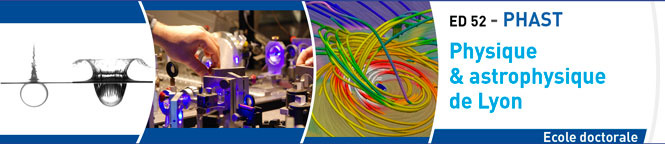
\includegraphics[width=0.5\textwidth]{logo-edphast.jpg}
    \end{center}
  \end{frame}
  
  \begin{frame}
  \frametitle{Sommaire}
    \tableofcontents
  \end{frame}   


%%%%%%%%%%%%%%%%%%
%% INTRODUCTION %%
%%%%%%%%%%%%%%%%%%


  %% Le prototype SDHCAL
  \section{The CALICE SDHCAL prototype}
  
  \begin{frame}
  \frametitle{The CALICE SDHCAL prototype}
  \framesubtitle{Description}
    \begin{minipage}{0.48\linewidth}
      \begin{block}{Semi-Digital Hadron Calorimeter}
        \begin{itemize}
          \item Sampling calorimeter
          \item 48 layers :
          \begin{itemize}
            \item Steel absorber
            \item Sensitive medium : GRPC
          \end{itemize}
          \item Segmentation :
          \begin{itemize}
            \item Transverse : 1 $cm^2$
            \item Longitudinal : 2.67 cm (abs. + sens)
          \end{itemize}
          \item Semi digital readout with 3 thresholds
        \end{itemize}
      \end{block}     
    \end{minipage} \hfill
    \begin{minipage}{0.48\linewidth}
      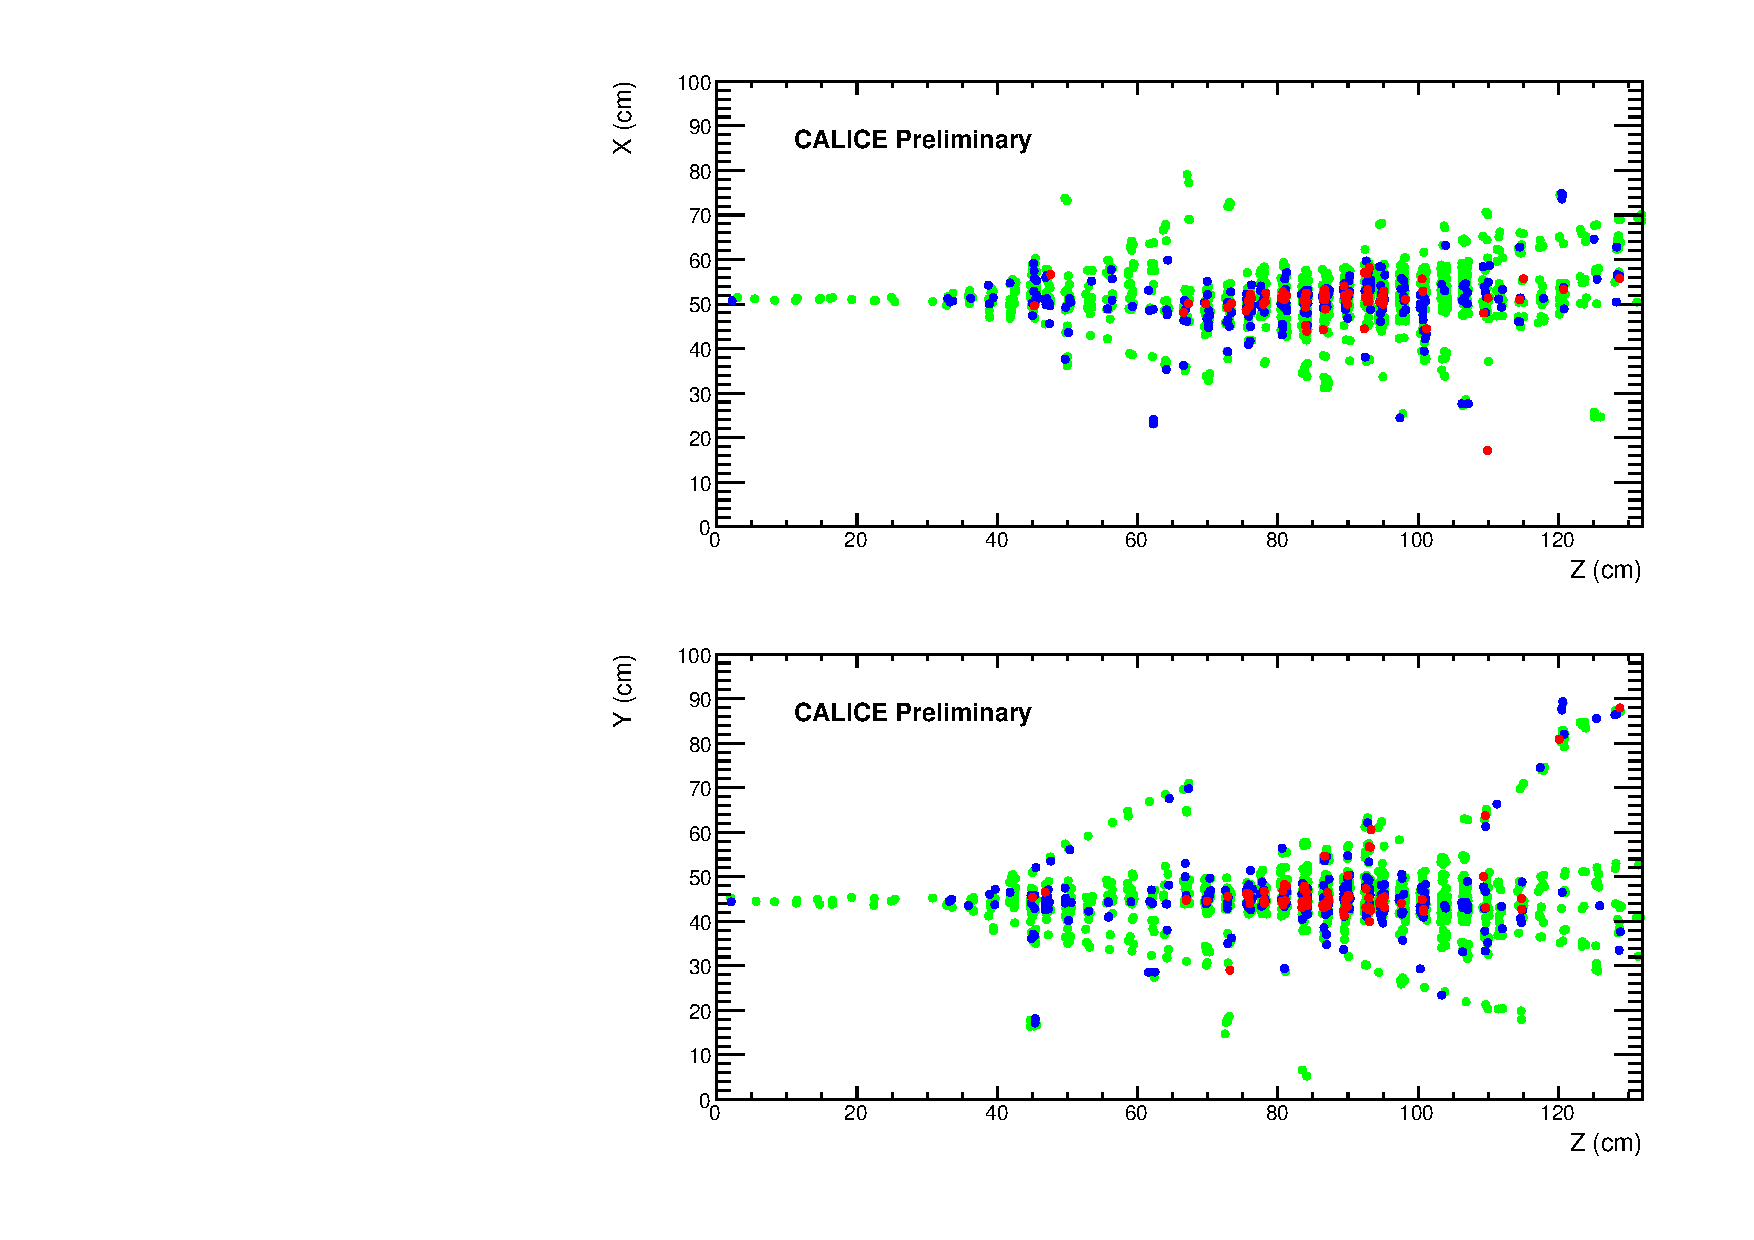
\includegraphics[width=\linewidth]{sdhcal_pion_80GeV.pdf}
    \end{minipage}
    \begin{minipage}{0.58\linewidth}
      \begin{center}
        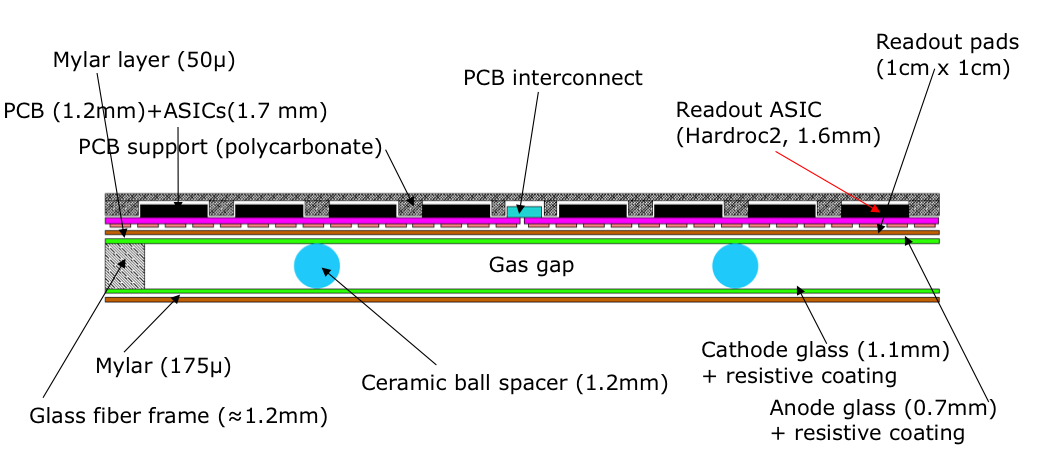
\includegraphics[width=0.9\linewidth]{GRPC-K7.png}      
      \end{center}
    \end{minipage} \hfill
    \begin{minipage}{0.4\linewidth}
      \begin{center}
        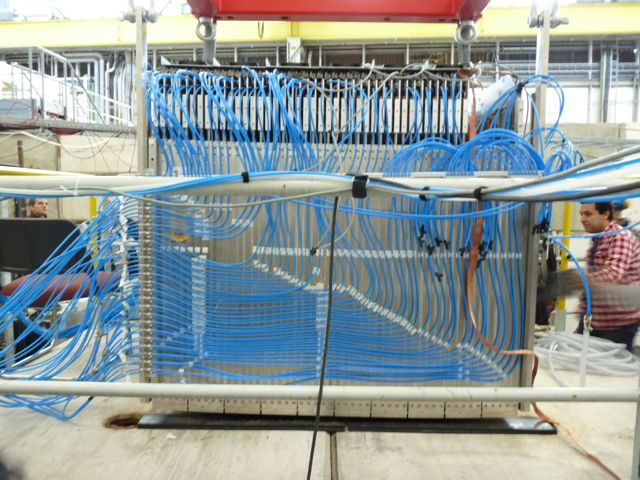
\includegraphics[width=0.7\linewidth]{sdhcal_testbeam.jpg}
      \end{center}
    \end{minipage}
  \end{frame}

    
  %% Multiplicité / Efficacité
  \begin{frame}
  \frametitle{The CALICE SDHCAL prototype}
  \framesubtitle{Performances}
    \begin{minipage}{0.48\linewidth}
      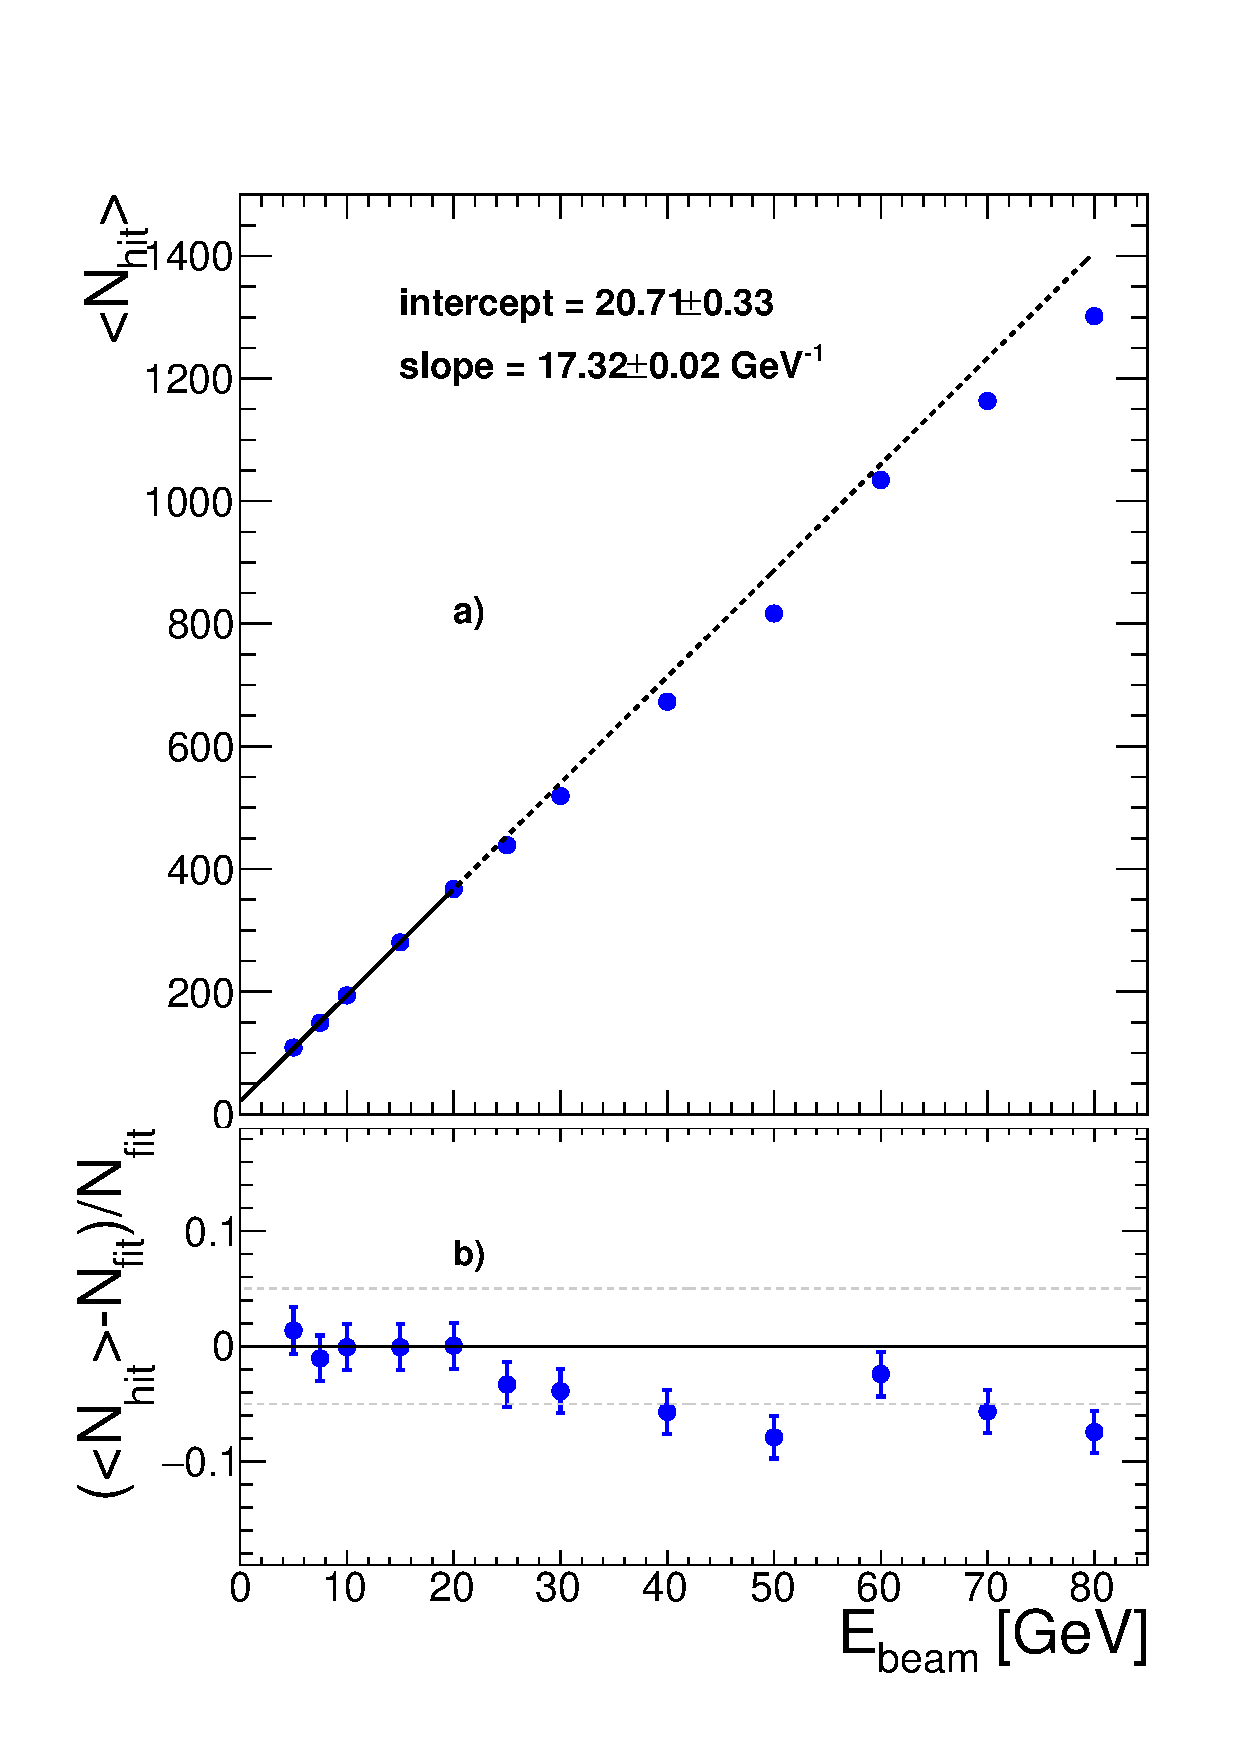
\includegraphics[width=1.2\linewidth]{NHITPION.pdf}
    \end{minipage} \hfill
    \begin{minipage}{0.48\linewidth}
      \begin{center}
        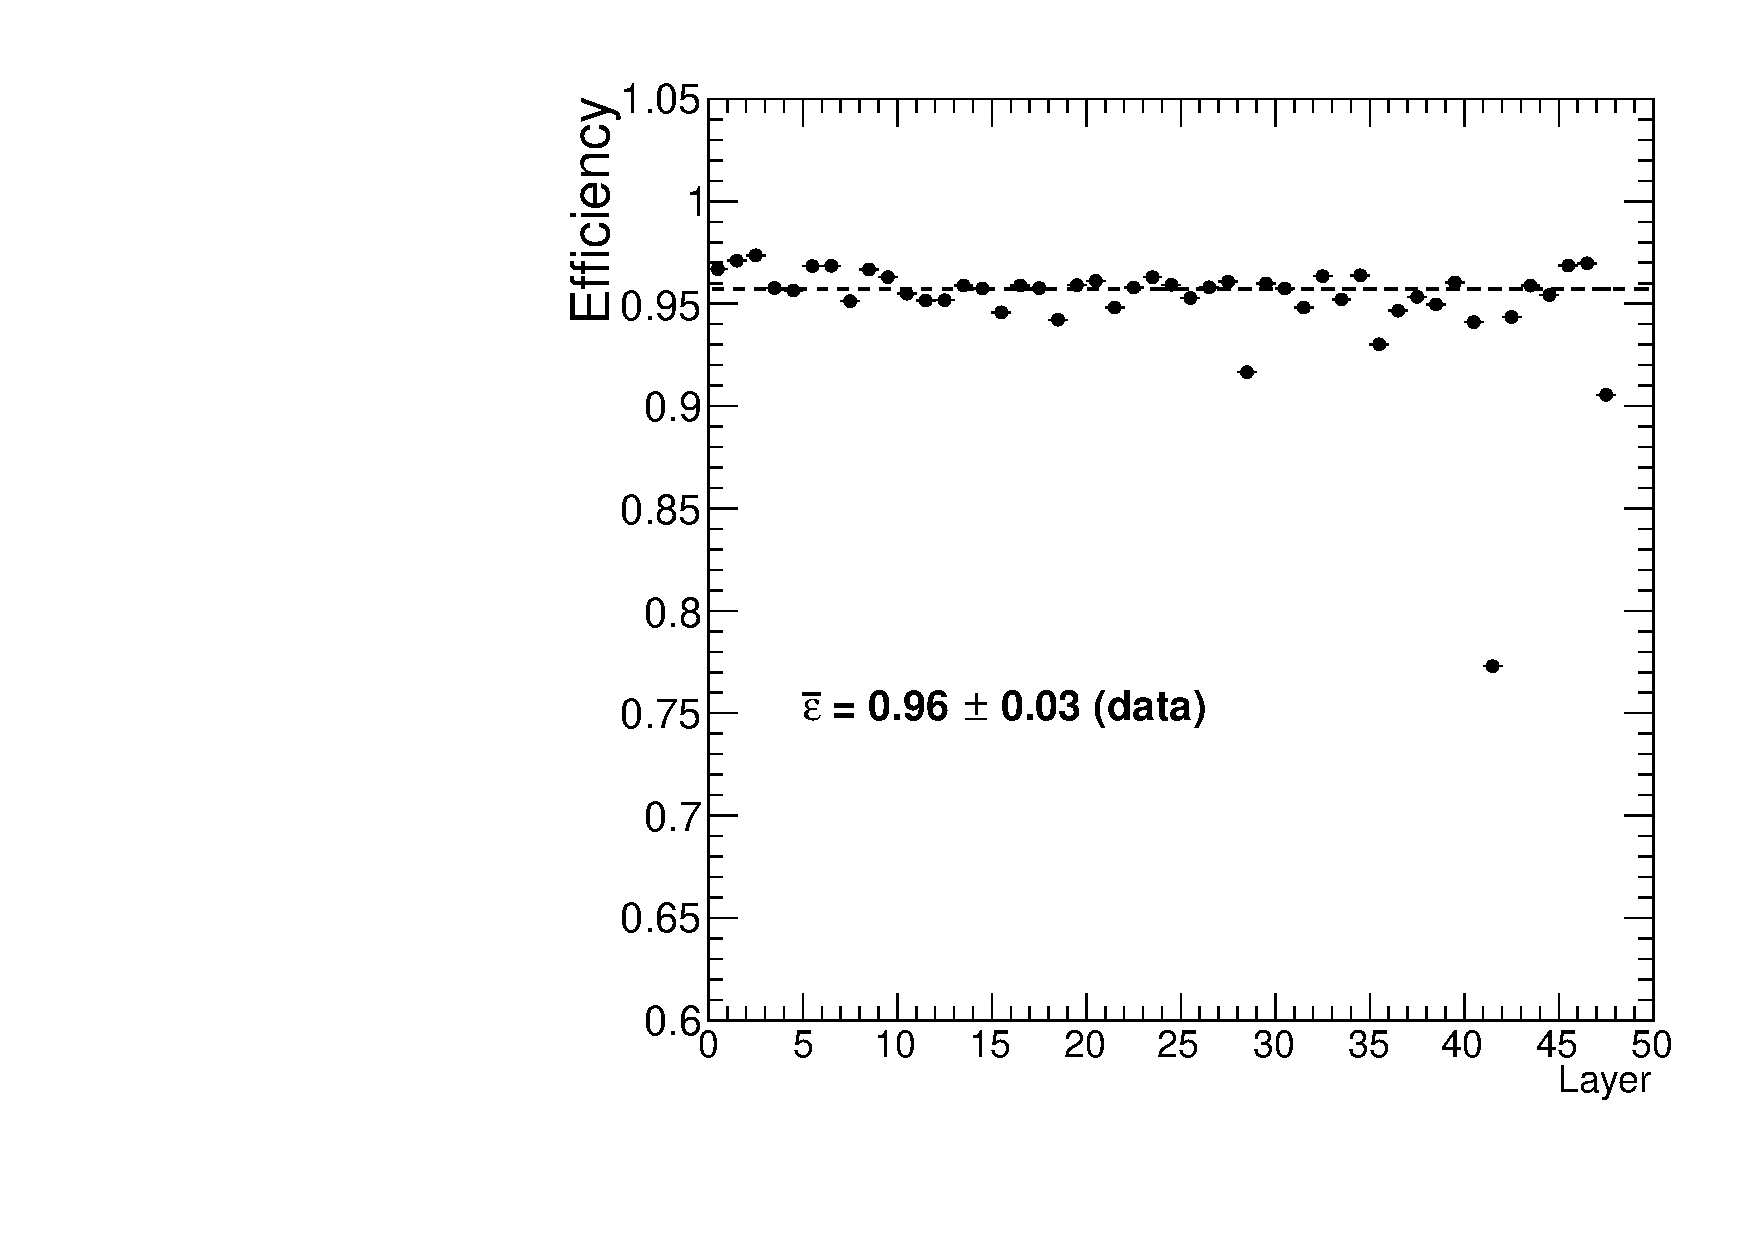
\includegraphics[width=0.7\linewidth]{eff_2012.pdf} \\
        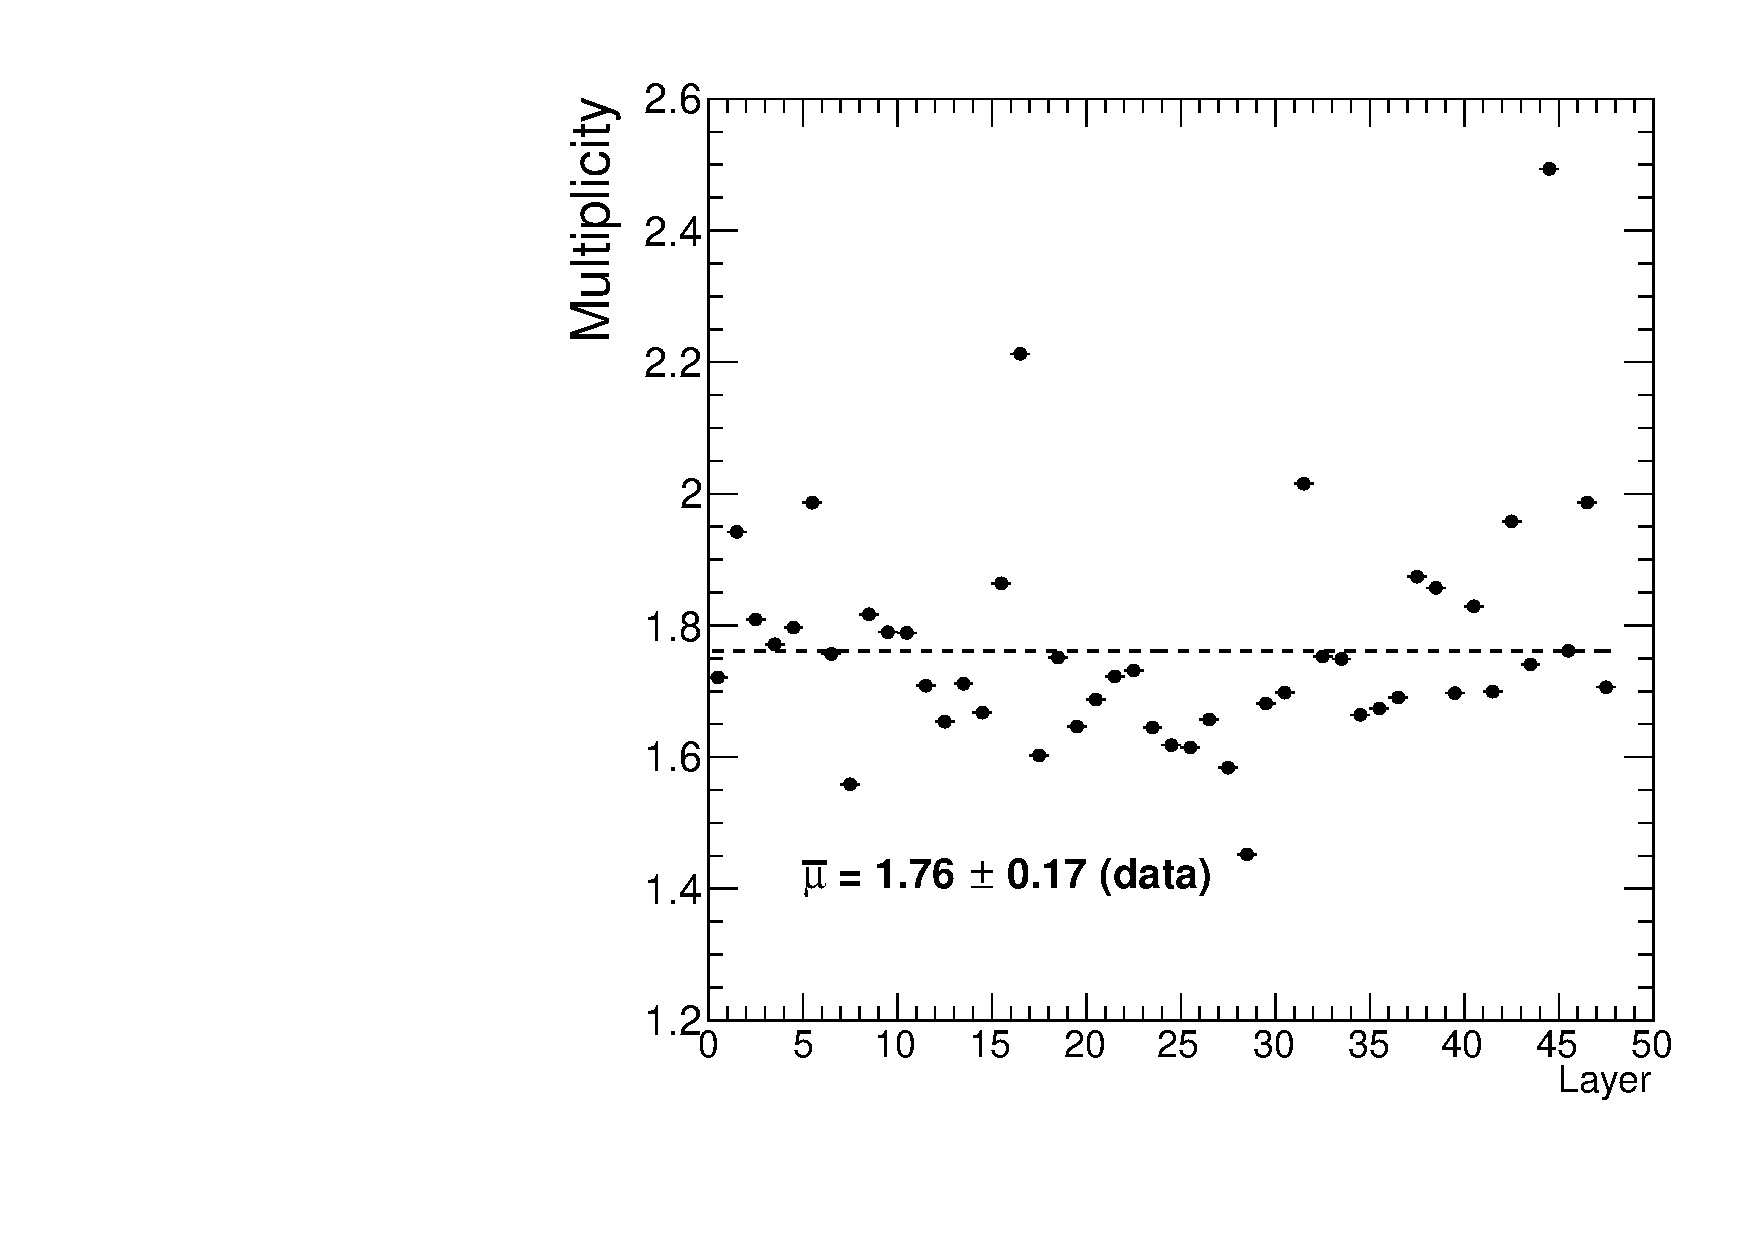
\includegraphics[width=0.7\linewidth]{mul_2012.pdf} \\
        A. Steen [CAN-053. EB]
      \end{center}
    \end{minipage}
  \end{frame}
  
  
  %% Reconstruction de l'énergie
  \begin{frame}
  \frametitle{The CALICE SDHCAL prototype}
  \framesubtitle{Performances}
    \begin{minipage}{0.48\linewidth}
      \begin{block}{Energy reconstruction}
        {\small
        \begin{equation}
          E = \alpha(NHit)\cdot N_1 + \beta(NHit)\cdot N_2 + \gamma(NHit)\cdot N_3 
        \end{equation}
        avec :
        \begin{equation}
          \alpha(NHit) = \alpha_1 + \alpha_2\cdot NHit + \alpha_3\cdot NHit^2
        \end{equation}
        \begin{equation}
          \beta(NHit) = \beta_1 + \beta_2\cdot NHit + \beta_3\cdot NHit^2
        \end{equation}
        \begin{equation}
          \gamma(NHit) = \gamma_1 + \gamma_2\cdot NHit + \gamma_3\cdot NHit^2
        \end{equation}
        }
      \end{block}
      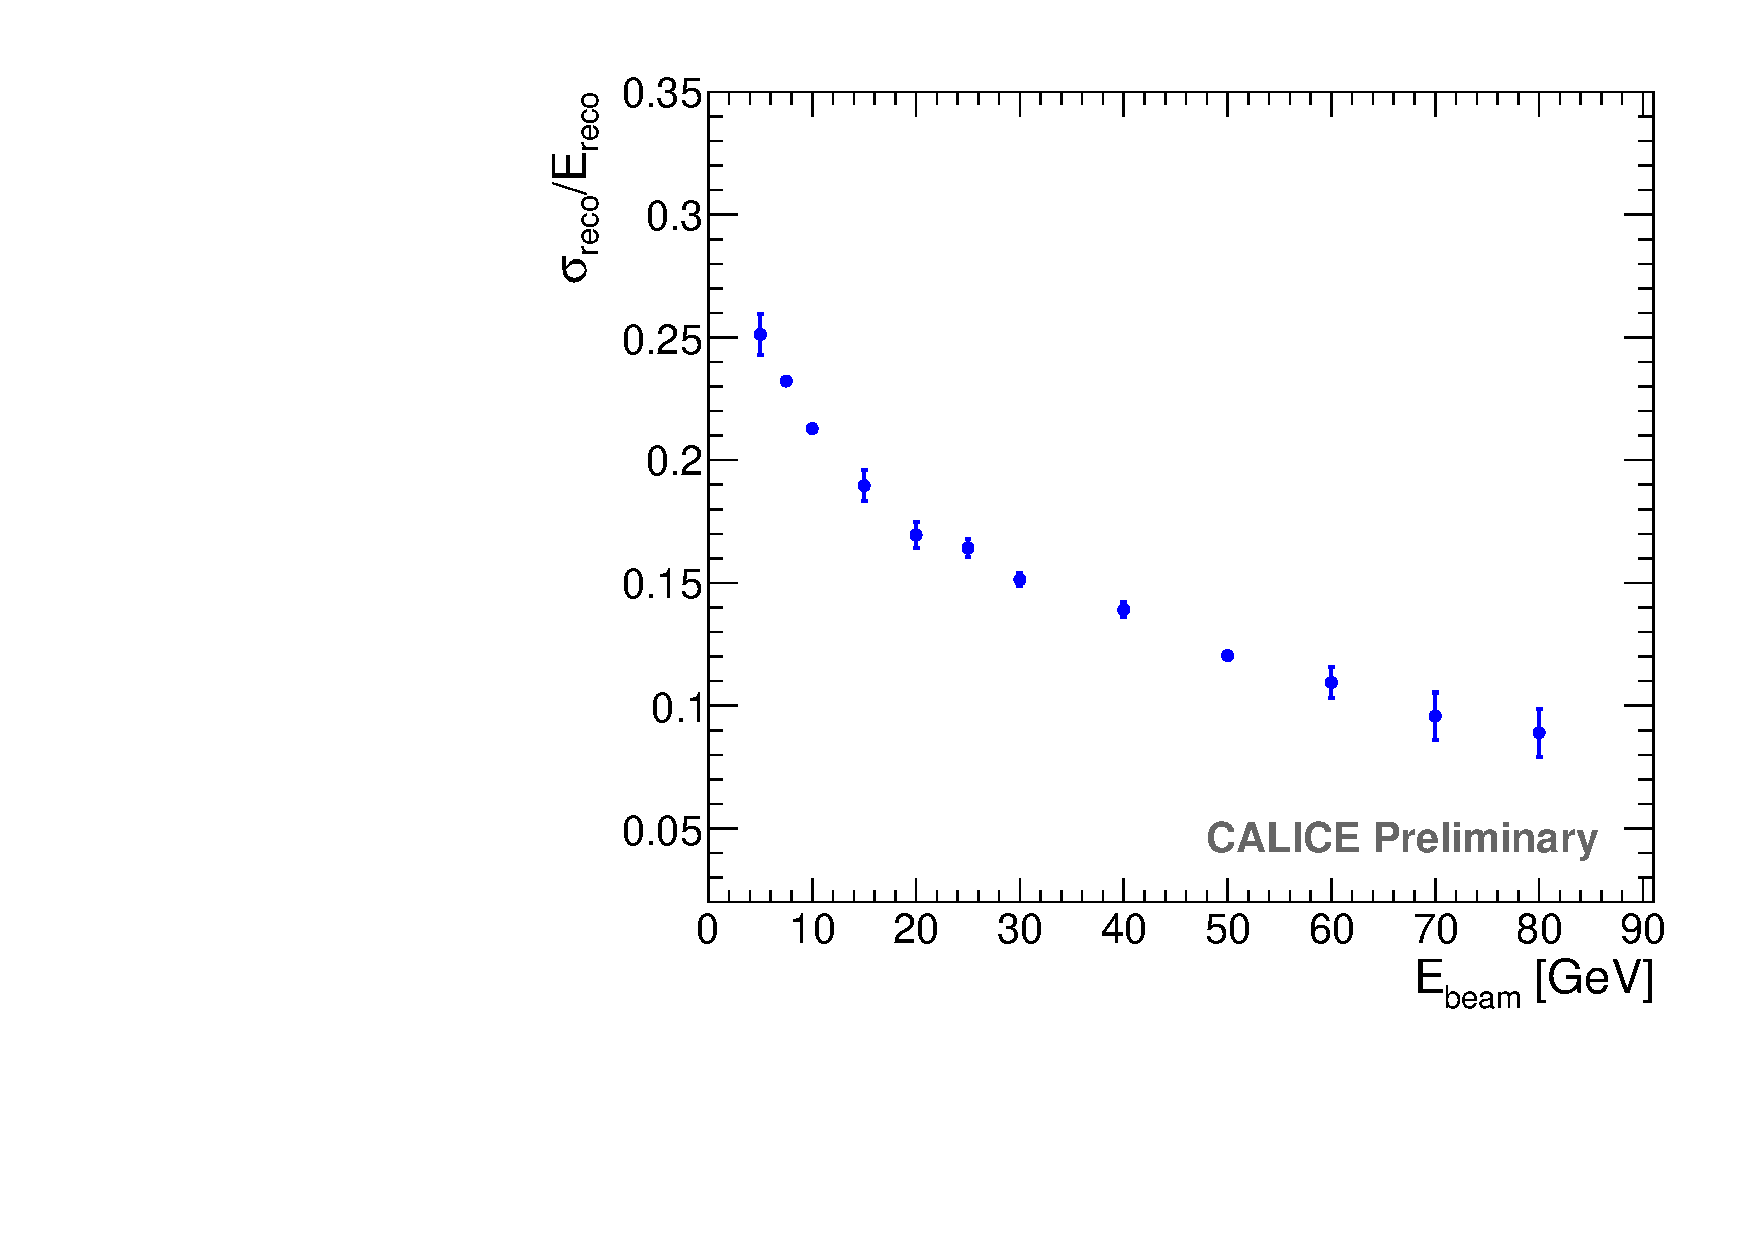
\includegraphics[width=\linewidth]{Energy-Resolution.pdf}
    \end{minipage} \hfill
    \begin{minipage}{0.5\linewidth}
      \begin{center}
        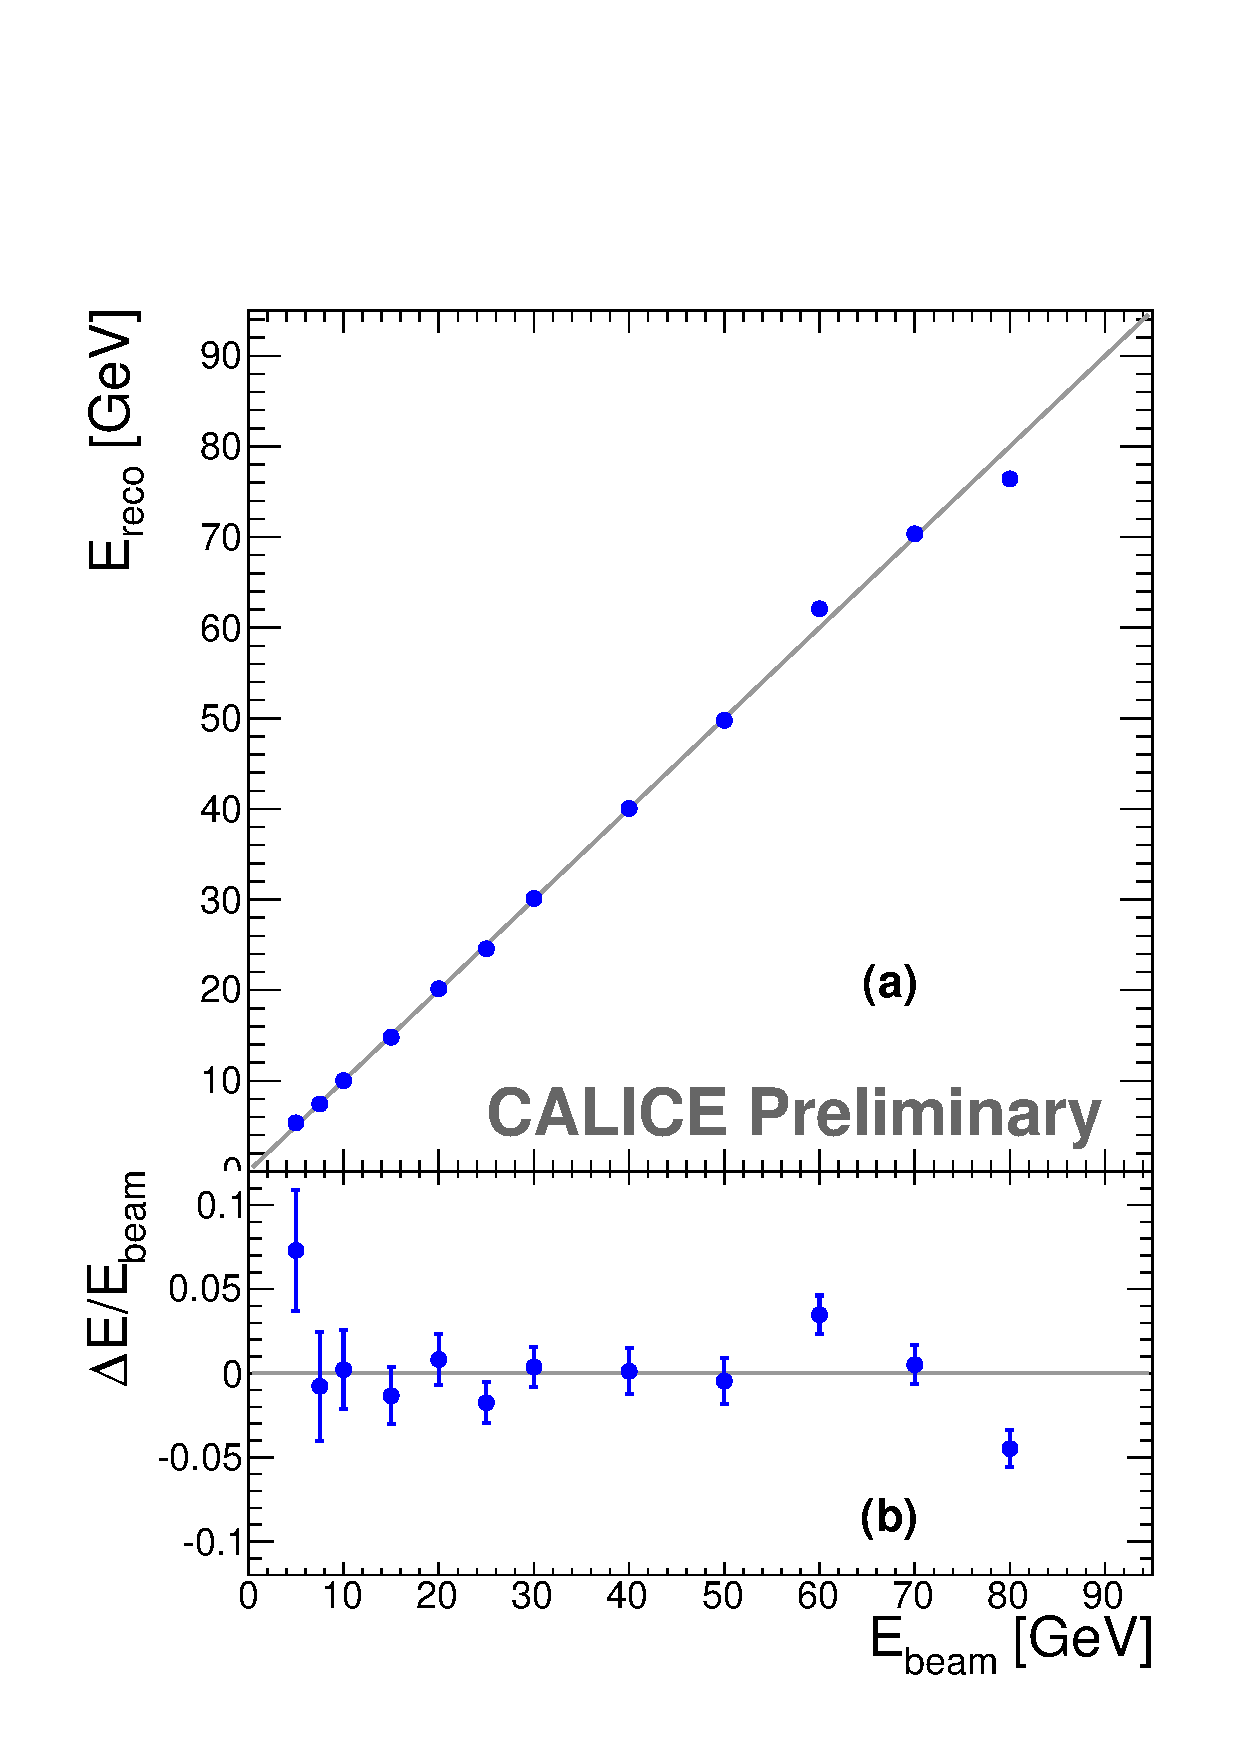
\includegraphics[width=\linewidth]{Energy-Linearity.pdf} \\
        Calice SDHCAL [CAN-037]
      \end{center}
    \end{minipage}
  \end{frame}
  
%%%%%%%%%%%%%%%%%
%% ALGO DE PFA %%
%%%%%%%%%%%%%%%%%
  \section{The Arbor Particle Flow Algorithm}
  
  %% ArborPFA
%  \subsection{ArborPFA}

  %% Principe  
  \begin{frame}
  \frametitle{ArborPFA}
  \framesubtitle{Principle}
    \begin{block}{Principle}
      Particle Flow Algorithm based on hadronic shower \textbf{tree-like topology}.
    \end{block}
    \pause
    \begin{minipage}{0.48\linewidth}
      \begin{center}
        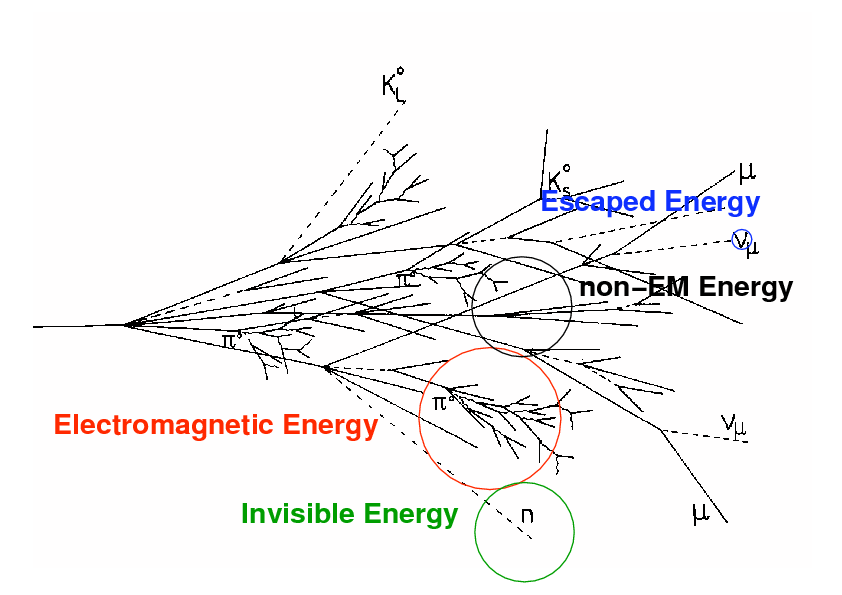
\includegraphics[width=0.8\linewidth]{hadronic_shower.png}      
      \end{center}
    \end{minipage} \hfill
    \begin{minipage}{0.48\linewidth}
      \begin{center}
        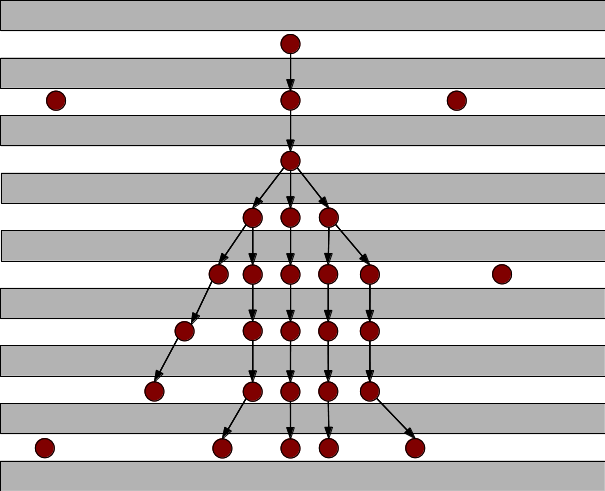
\includegraphics[angle=90, width=0.5\linewidth]{ArborSchema.png}        
      \end{center}
    \end{minipage}
    \pause
    \begin{block}{Some definitions}
      \begin{itemize}
        \item \textbf{Object} : \textit{Node} linked by one or many connector(s) (+ seeds and leafs)
        \item \textbf{Connector} : Oriented \textit{link}. Links two objects
        \item \textbf{Flow direction} : Connector orientation, backward or forward
        \item \textbf{Tree} : Set of objects linked by connectors. For each object :
        \begin{itemize}
          \item 0 or 1 backward connector
          \item 0 or many forward connector(s)
        \end{itemize}
        $\rightarrow$ Implies a unique tree structure solution (1 seed per tree)
      \end{itemize}
    \end{block}
  \end{frame}
  
  
  %% Description des algos 1
  \begin{frame}
  \frametitle{ArborPFA}
  \framesubtitle{The algorithms}
%    \begin{minipage}{0.48\linewidth}
      \begin{block}{\textcircled{{\small 1}} Object creation}
        $\blacksquare$ Create objects, ready to be connected.
        \begin{itemize}
          \item Nearest Neigbours clustering in each layer
          \item If cluster size <= 4, cluster = 1 object
          \item If cluster > 4, each cluster hit = 1 object
        \end{itemize}
        Allows to :
        \begin{itemize}
          \item to do not care about the multiplicity in gaseous calorimeters
          \item decrease the size of the problem. NHit $\rightarrow$ NObject (< NHit)
          \item accelerate the connection procedure
        \end{itemize}
      \end{block}
 %   \end{minipage} \hfill
  %  \begin{minipage}{0.48\linewidth}
      \begin{center}
      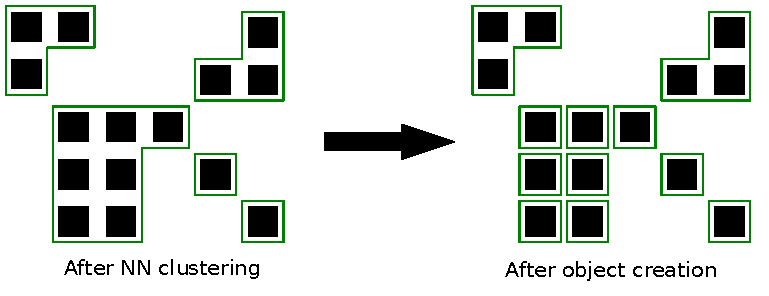
\includegraphics[width=0.7\linewidth]{ObjectCreation.pdf}
      \end{center}

   % \end{minipage}
  \end{frame}
  
  
  %% Description des algos 2
  \begin{frame}
  \frametitle{ArborPFA}
  \framesubtitle{The algorithms}
    \begin{block}{Tree building}
      Iteration phase :
      \begin{itemize}
        \item Connector creation between objects (seeding)
        \item Connector cleaning to obtain a tree structure (cleaning)
      \end{itemize}
      ~ \\
      Repeat the two previous algorithms as much as needed. \\ ~ \\
      \underline{Global idea} : create an initial tree structure to start with. Then alterate the latter by creating more optimized connections.
    \end{block}
  \end{frame}
  
  
  %% Description des algos 3
  \begin{frame}
  \frametitle{ArborPFA}
  \framesubtitle{The algorithms}
    \begin{block}{\textcircled{{\small 2}} Connector creation 1}
      $\blacksquare$ 
      For each object, we look for nearby objects in the 3 next layers within a distance of 45 mm. A connection is then created for each of them.
    \end{block}
    \begin{center}
      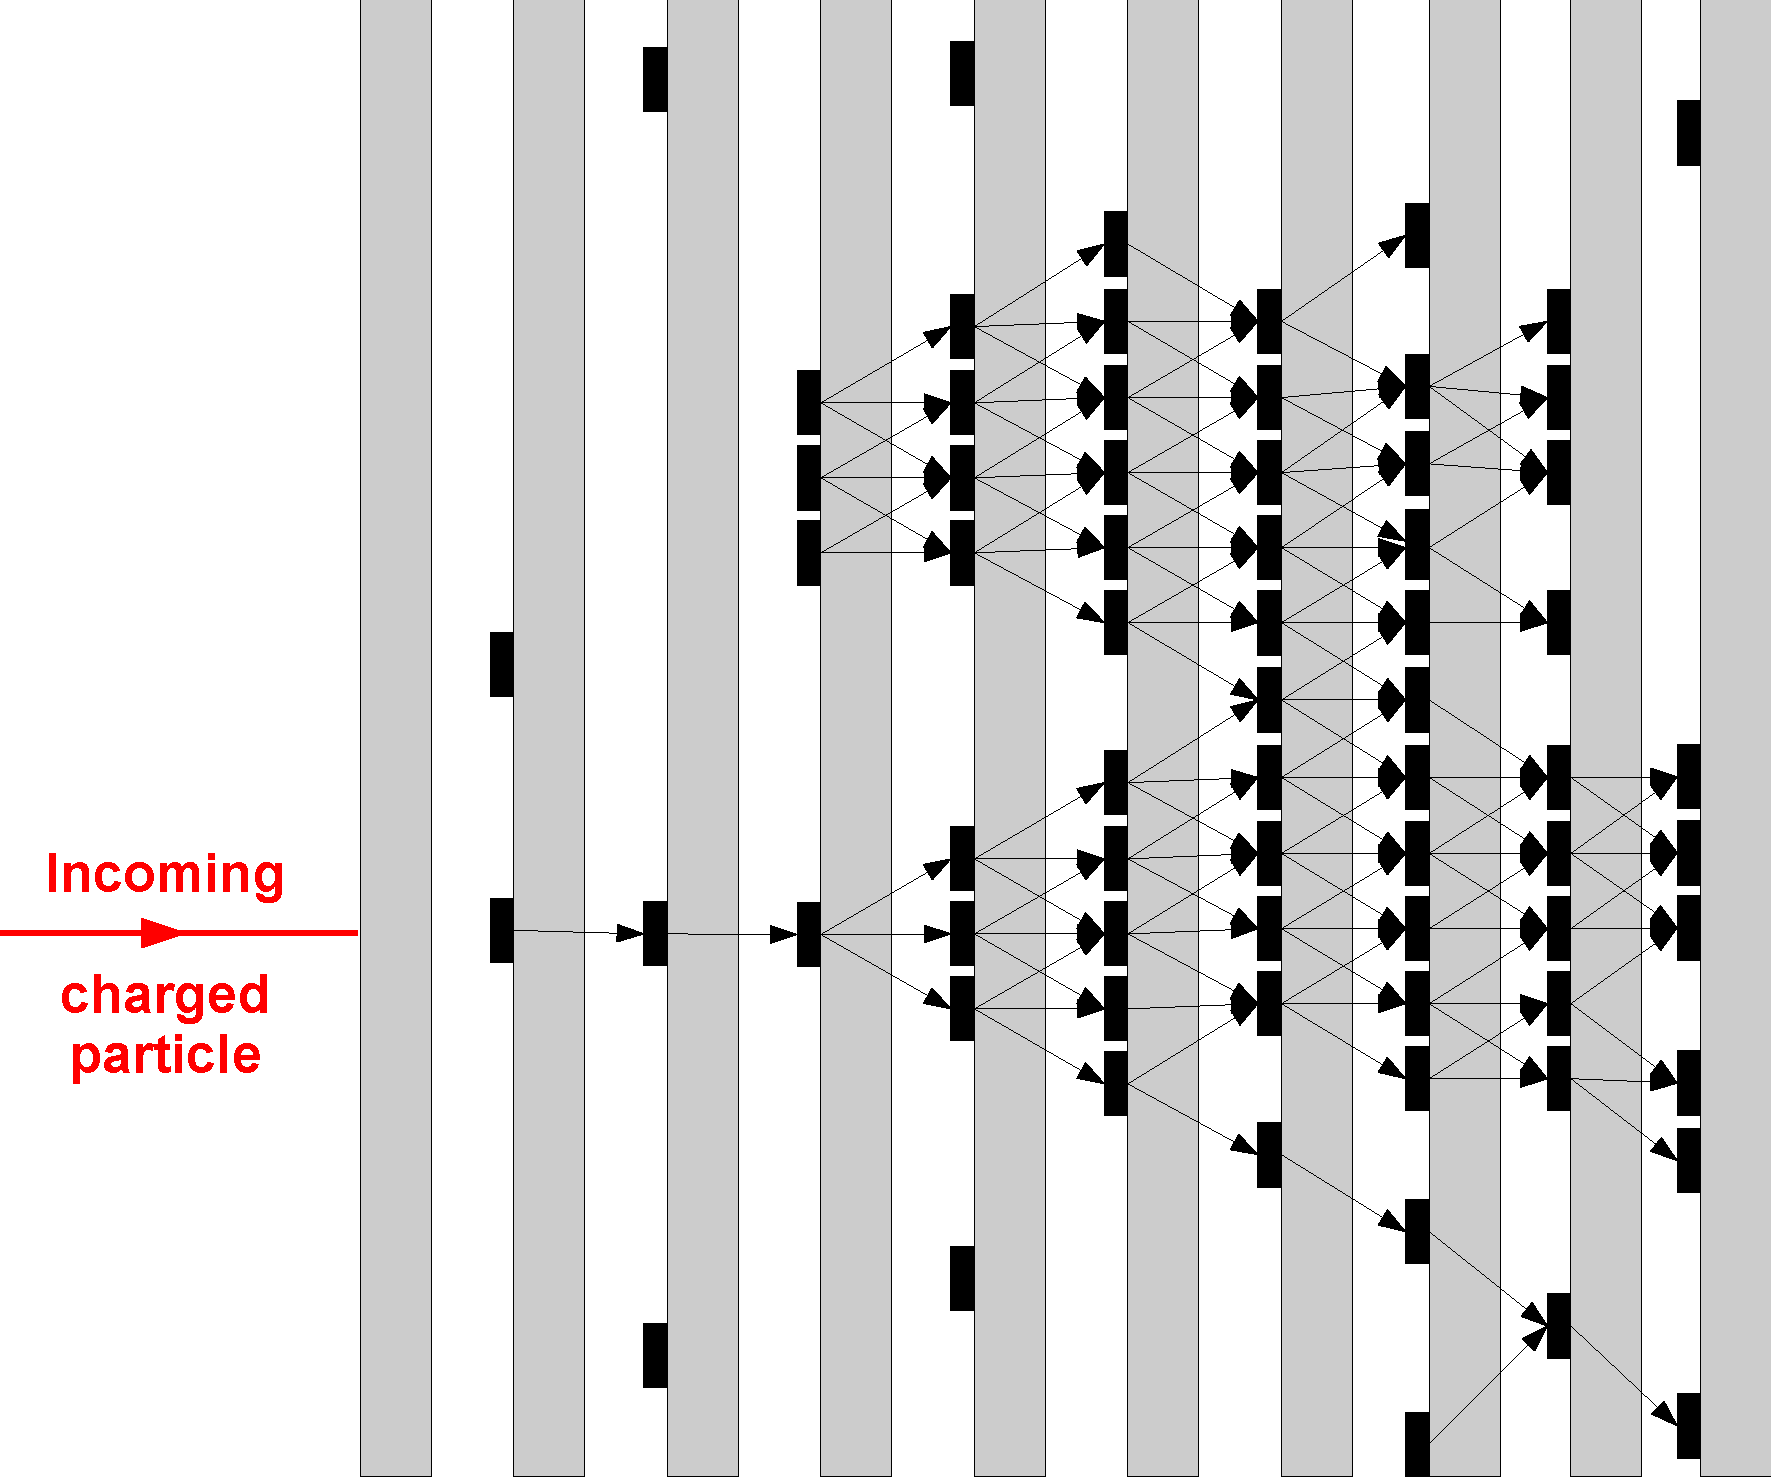
\includegraphics[width=0.6\linewidth]{ConnectorSeeding1.pdf} \\ ~ \\
    \end{center}
  \end{frame}
  
  
    %% Description des algos 3
  \begin{frame}
  \frametitle{ArborPFA}
  \framesubtitle{The algorithms}
    \begin{minipage}{0.55\linewidth}
      \begin{block}{\textcircled{{\small 3}} Connector cleaning 1}
        \onslide<1->{$\blacksquare$ Clean connectors to create a tree structure.} \\
        \onslide<2->{For each object :}
        \begin{itemize}
          \item<3-> Computation of the reference direction :
          \begin{equation}
            \vec{C}_{ref} = w_{bck} . \sum_\sigma \sum_b \vec{c}_{b,\sigma} - w_{fwd} . \sum_\delta \sum_f \vec{c}_{f,\delta}
          \end{equation}
          \item<4-> For each object in the backward direction, we define the $\kappa$ order parameter :
          \begin{equation}
            \kappa~=~\Big(\frac{\theta}{\pi}\Big)^{p_{\theta}} . ~\Big(\frac{\Delta}{\Delta_{max}}\Big)^{p_{\Delta}} 
          \end{equation}
          \item<5-> The connector with the smallest $\kappa$ is kept.
          \item<6-> \textbf{At the end of the algorithm}, the other connectors are deleted. \\
        \end{itemize}
        \onslide<7->{$\rightarrow$ Formation of a tree structure.}
      \end{block}
    \end{minipage} \hfill
    \begin{minipage}{0.3\linewidth}
      \begin{center}
        \begin{overlayarea}{\linewidth}{\linewidth}
          \includegraphics[width=1.1\linewidth]<2>{ConnectorCleaningExample1.pdf}
          \includegraphics[width=1.1\linewidth]<3>{ConnectorCleaningExample2.pdf}
          \includegraphics[width=1.1\linewidth]<4>{ConnectorCleaningExample3.pdf}
          \includegraphics[width=1.1\linewidth]<5>{ConnectorCleaningExample4.pdf}
          \includegraphics[width=1.1\linewidth]<6->{ConnectorCleaningExample5.pdf}      
        \end{overlayarea}
      \end{center}
    \end{minipage}
  \end{frame}
  
  %% Description des algos 4
  \begin{frame}
  \frametitle{ArborPFA}
  \framesubtitle{The algorithms}
    \begin{block}{\textcircled{{\small 4}} et \textcircled{{\small 5}} Connector alignment}
      $\blacksquare$ From the latest tree structure, more connections are created. This creates an alignment within the shower. A second connector cleaning is then performed to obtain a final tree structure.
    \end{block}
    \begin{center}
      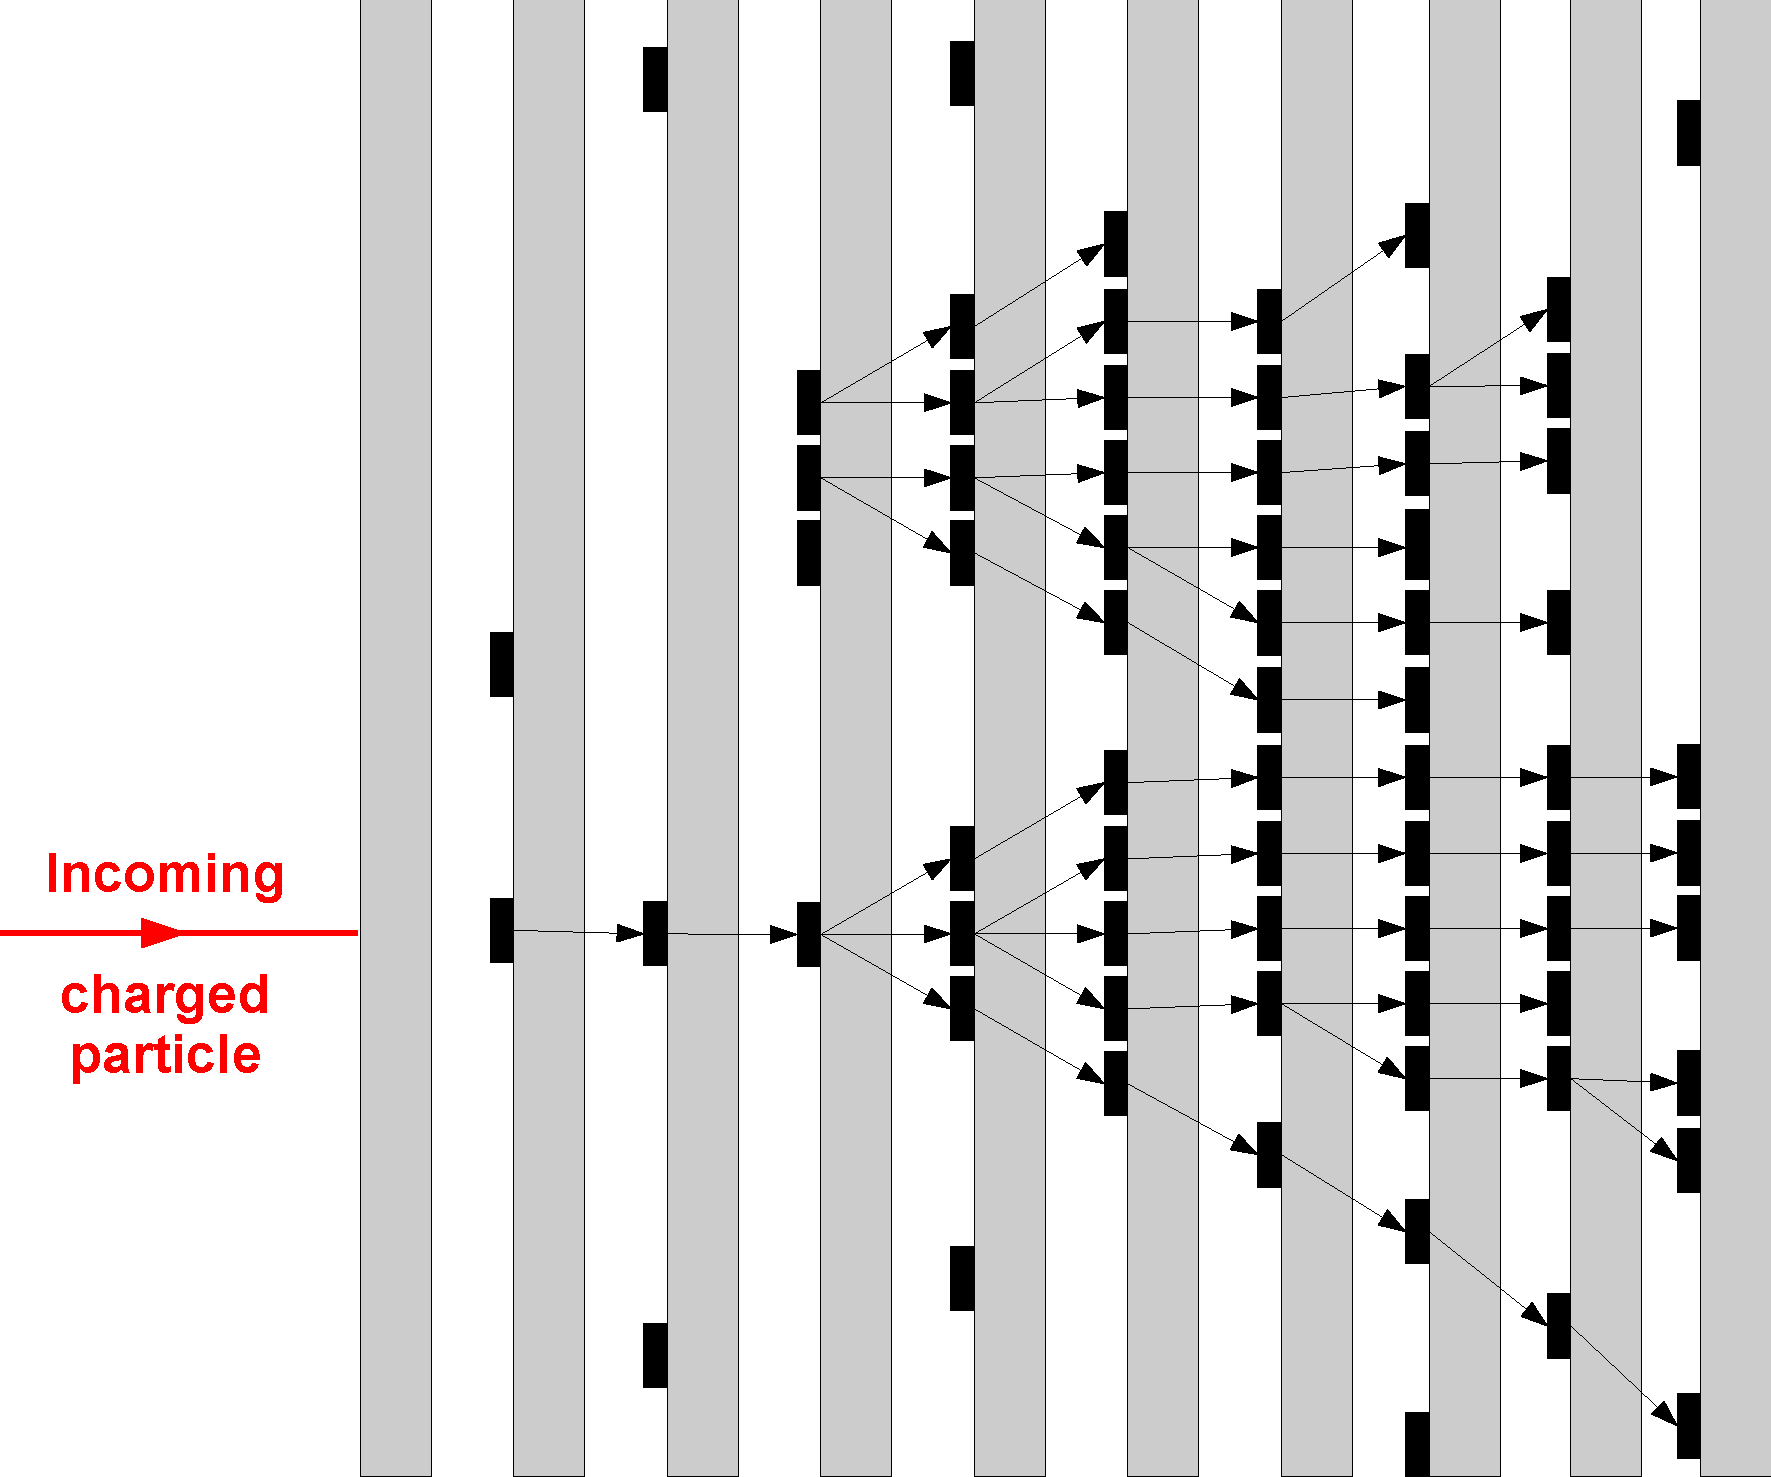
\includegraphics[width=0.6\linewidth]{ConnectorCleaning2.pdf}      
    \end{center}
  \end{frame}
  
  %% Description des algos 5
  \begin{frame}
  \frametitle{ArborPFA}
  \framesubtitle{The algorithms}
    \begin{minipage}{0.55\linewidth}
      \begin{block}{\textcircled{{\small 6}} Track-to-tree association}
        $\blacksquare$ Association between tracks and trees performed with simple criteria :
        \begin{itemize}
          \item Distance between a tree seed and track extrapolation to the calorimeter front face.
          \item Track momentum - tree energy comparison
          \item Handling of special cases as early interactions
        \end{itemize}
      \end{block}
      \begin{block}{\textcircled{{\small 7}} Neutral tree merging}
        $\blacksquare$ Interaction of neutral particles in an absorber. \\
        $\rightarrow$ Many seeds in the same layer, thus many reconstructed trees instead of a single one. \\
        Seeds belonging to this kind of configuration are \textbf{identified} and their trees \textbf{merged}.  
      \end{block}
    \end{minipage} \hfill
    \begin{minipage}{0.44\linewidth}
      \begin{center}
        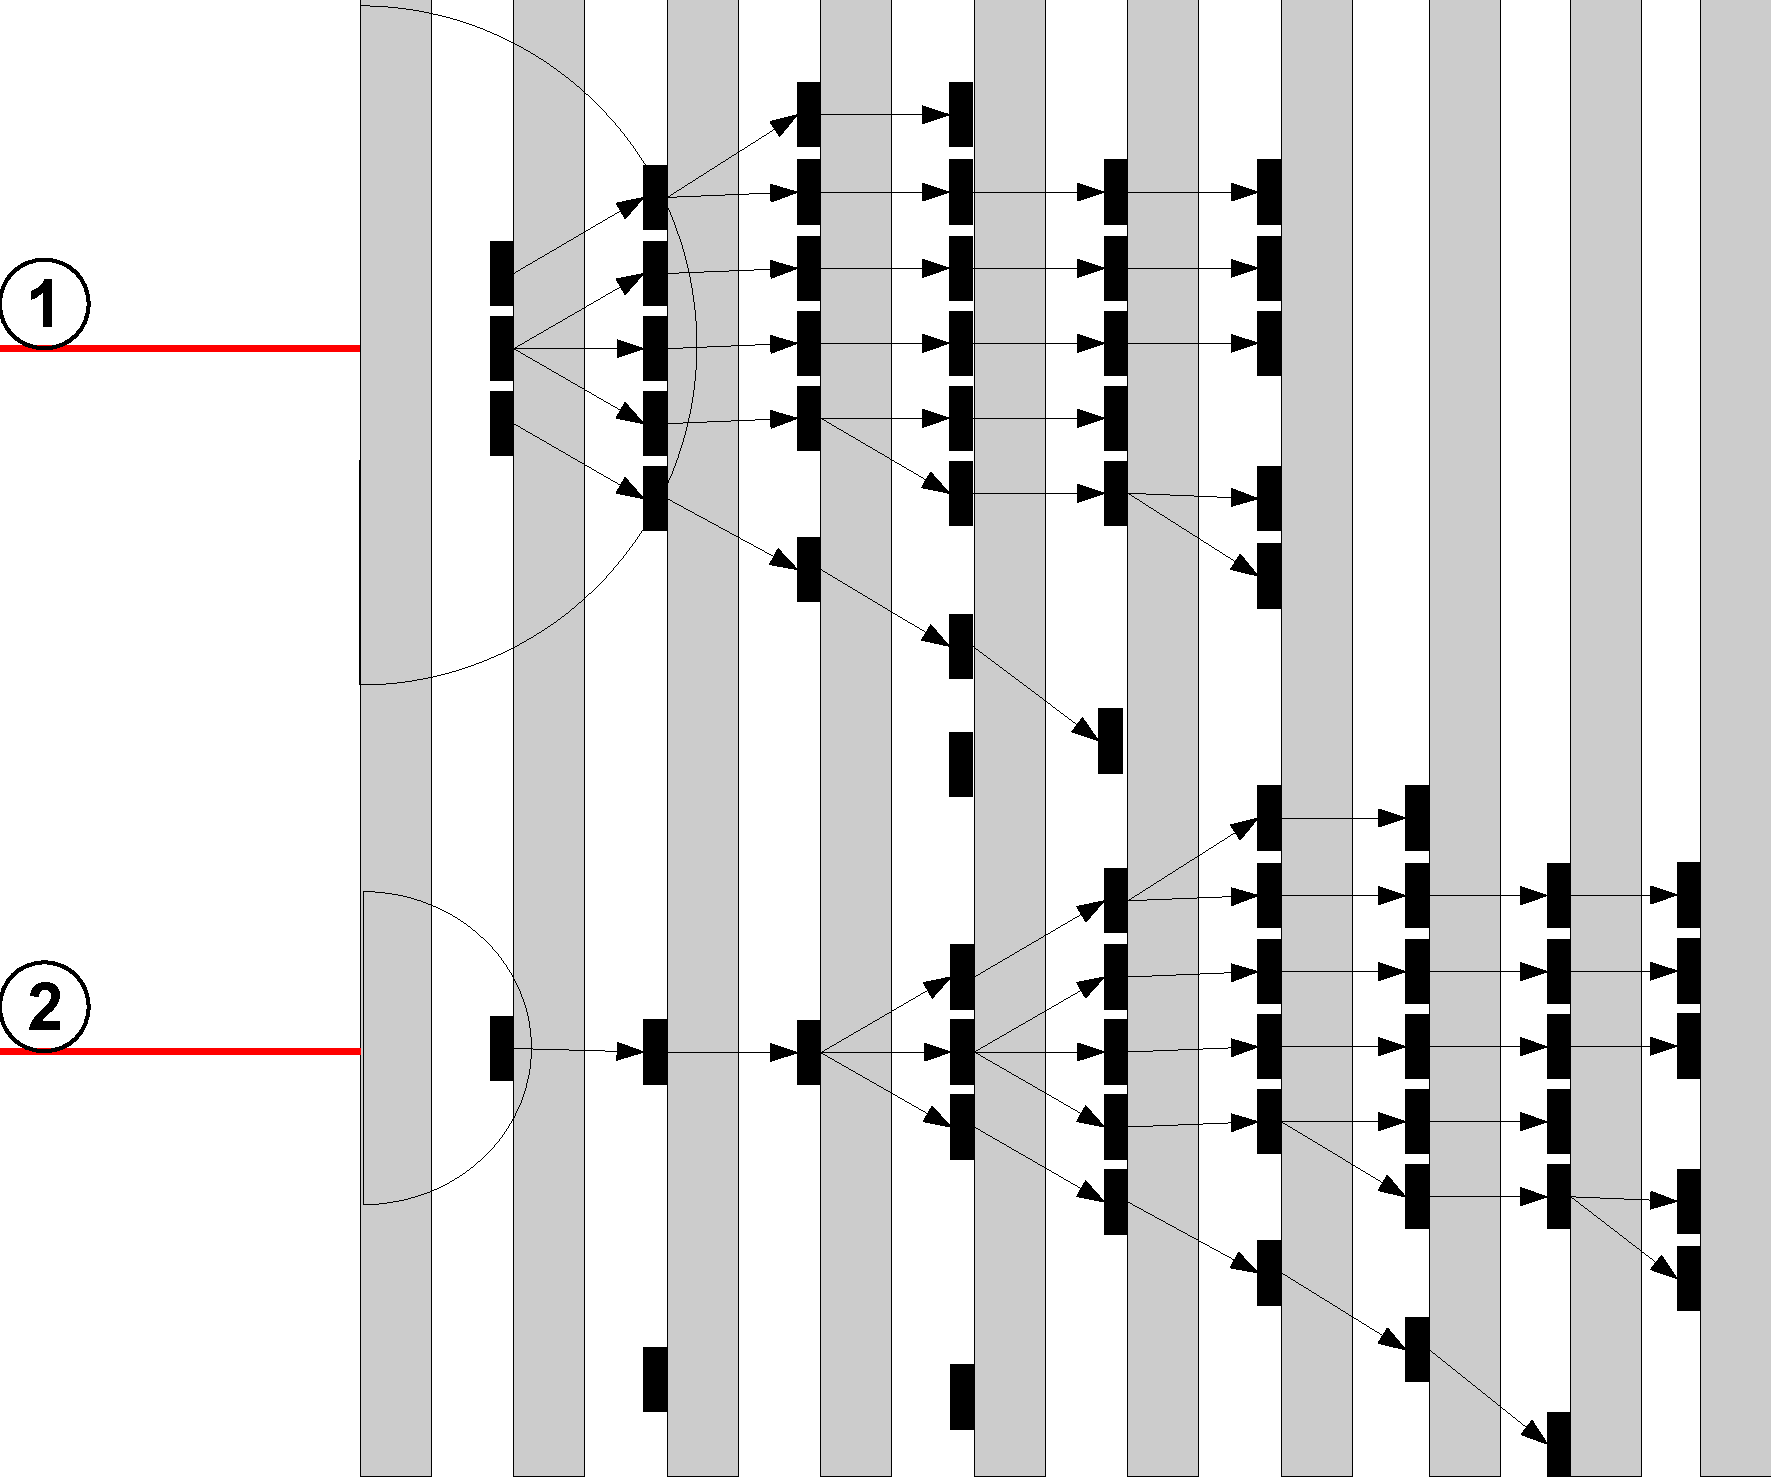
\includegraphics[width=0.9\linewidth]{EnergyDrivenTrackClusterAssociation.pdf} \\
        ~ \\
        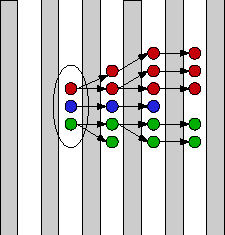
\includegraphics[width=0.5\linewidth]{NeutralTreeMerging.pdf}
      \end{center}
    \end{minipage}
  \end{frame}
  

  %% Description des algos 6
  \begin{frame}
  \frametitle{ArborPFA}
  \framesubtitle{The algorithms}
    \begin{minipage}{0.55\linewidth}
      \begin{block}{\textcircled{{\footnotesize 8}} Pointing trees association}
        $\blacksquare$ Association between neutral (daughter) trees and charged or neutral (parent) trees as a function of their main axis (3D linear fit over object positions) and their energies.
        \begin{itemize}
          \item D.c.a between axes.
          \item D.c.a between axis and barycentre
          \item Energy criteria (charged parent tree case)
        \end{itemize}
      \end{block}
      \begin{block}{\textcircled{{\footnotesize 9}} Small neutral tree merging}
        $\blacksquare$ Small trees (NObj < 20) are merged in the closest bigger tree (NObj $\geq$ 20).
      \end{block}
    \end{minipage} \hfill
    \begin{minipage}{0.415\linewidth}
      \begin{center}
        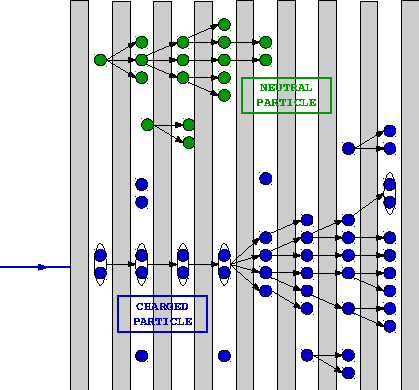
\includegraphics[width=\linewidth]{PfoCreation.pdf}
      \end{center}
      \begin{block}{\textcircled{{\footnotesize 10}} \textit{Particle Flow Objects} creation}
        $\blacksquare$ Creation of reconstructed particles :
        \begin{itemize}
          \item one track (if charged particle)
          \item one tree
        \end{itemize}
      \end{block} 
    \end{minipage}
  \end{frame}
  
  
  \section{Algorithm performances}
  
  %% Performance ArborPFA - single particle
  \subsection{Single particle performances}
  
  \begin{frame}
  \frametitle{Single particle reconstruction}
%  \framesubtitle{\subsecname}
    \begin{minipage}{0.56\linewidth}
      \begin{block}{Reconstruction inputs}
        \begin{itemize}
          \item Data : CERN SPS 2012 - August-September \\
          \item Particles : $h^{\pm}$
          \item Energies : [10 ; 80] GeV by steps of 10 GeV
          \item "Fake" track generated : 
          \begin{itemize}
            \item $\vec{p}$ = (0, 0, $E_{beam}$)
            \item Entry point $\vec{e}$ : barycentre ($b_x$, $b_y$) of hits in the 5 first layers \\
            $\rightarrow$ $\vec{e}$ = (b$_x$, b$_y$, z$_{front}$)
          \end{itemize}
          \item No magnetic field ($\vec{B}$ = $\vec{0}$ T)
        \end{itemize}
      \end{block}
    \end{minipage} \hfill
    \begin{minipage}{0.43\linewidth}
      \begin{center}
        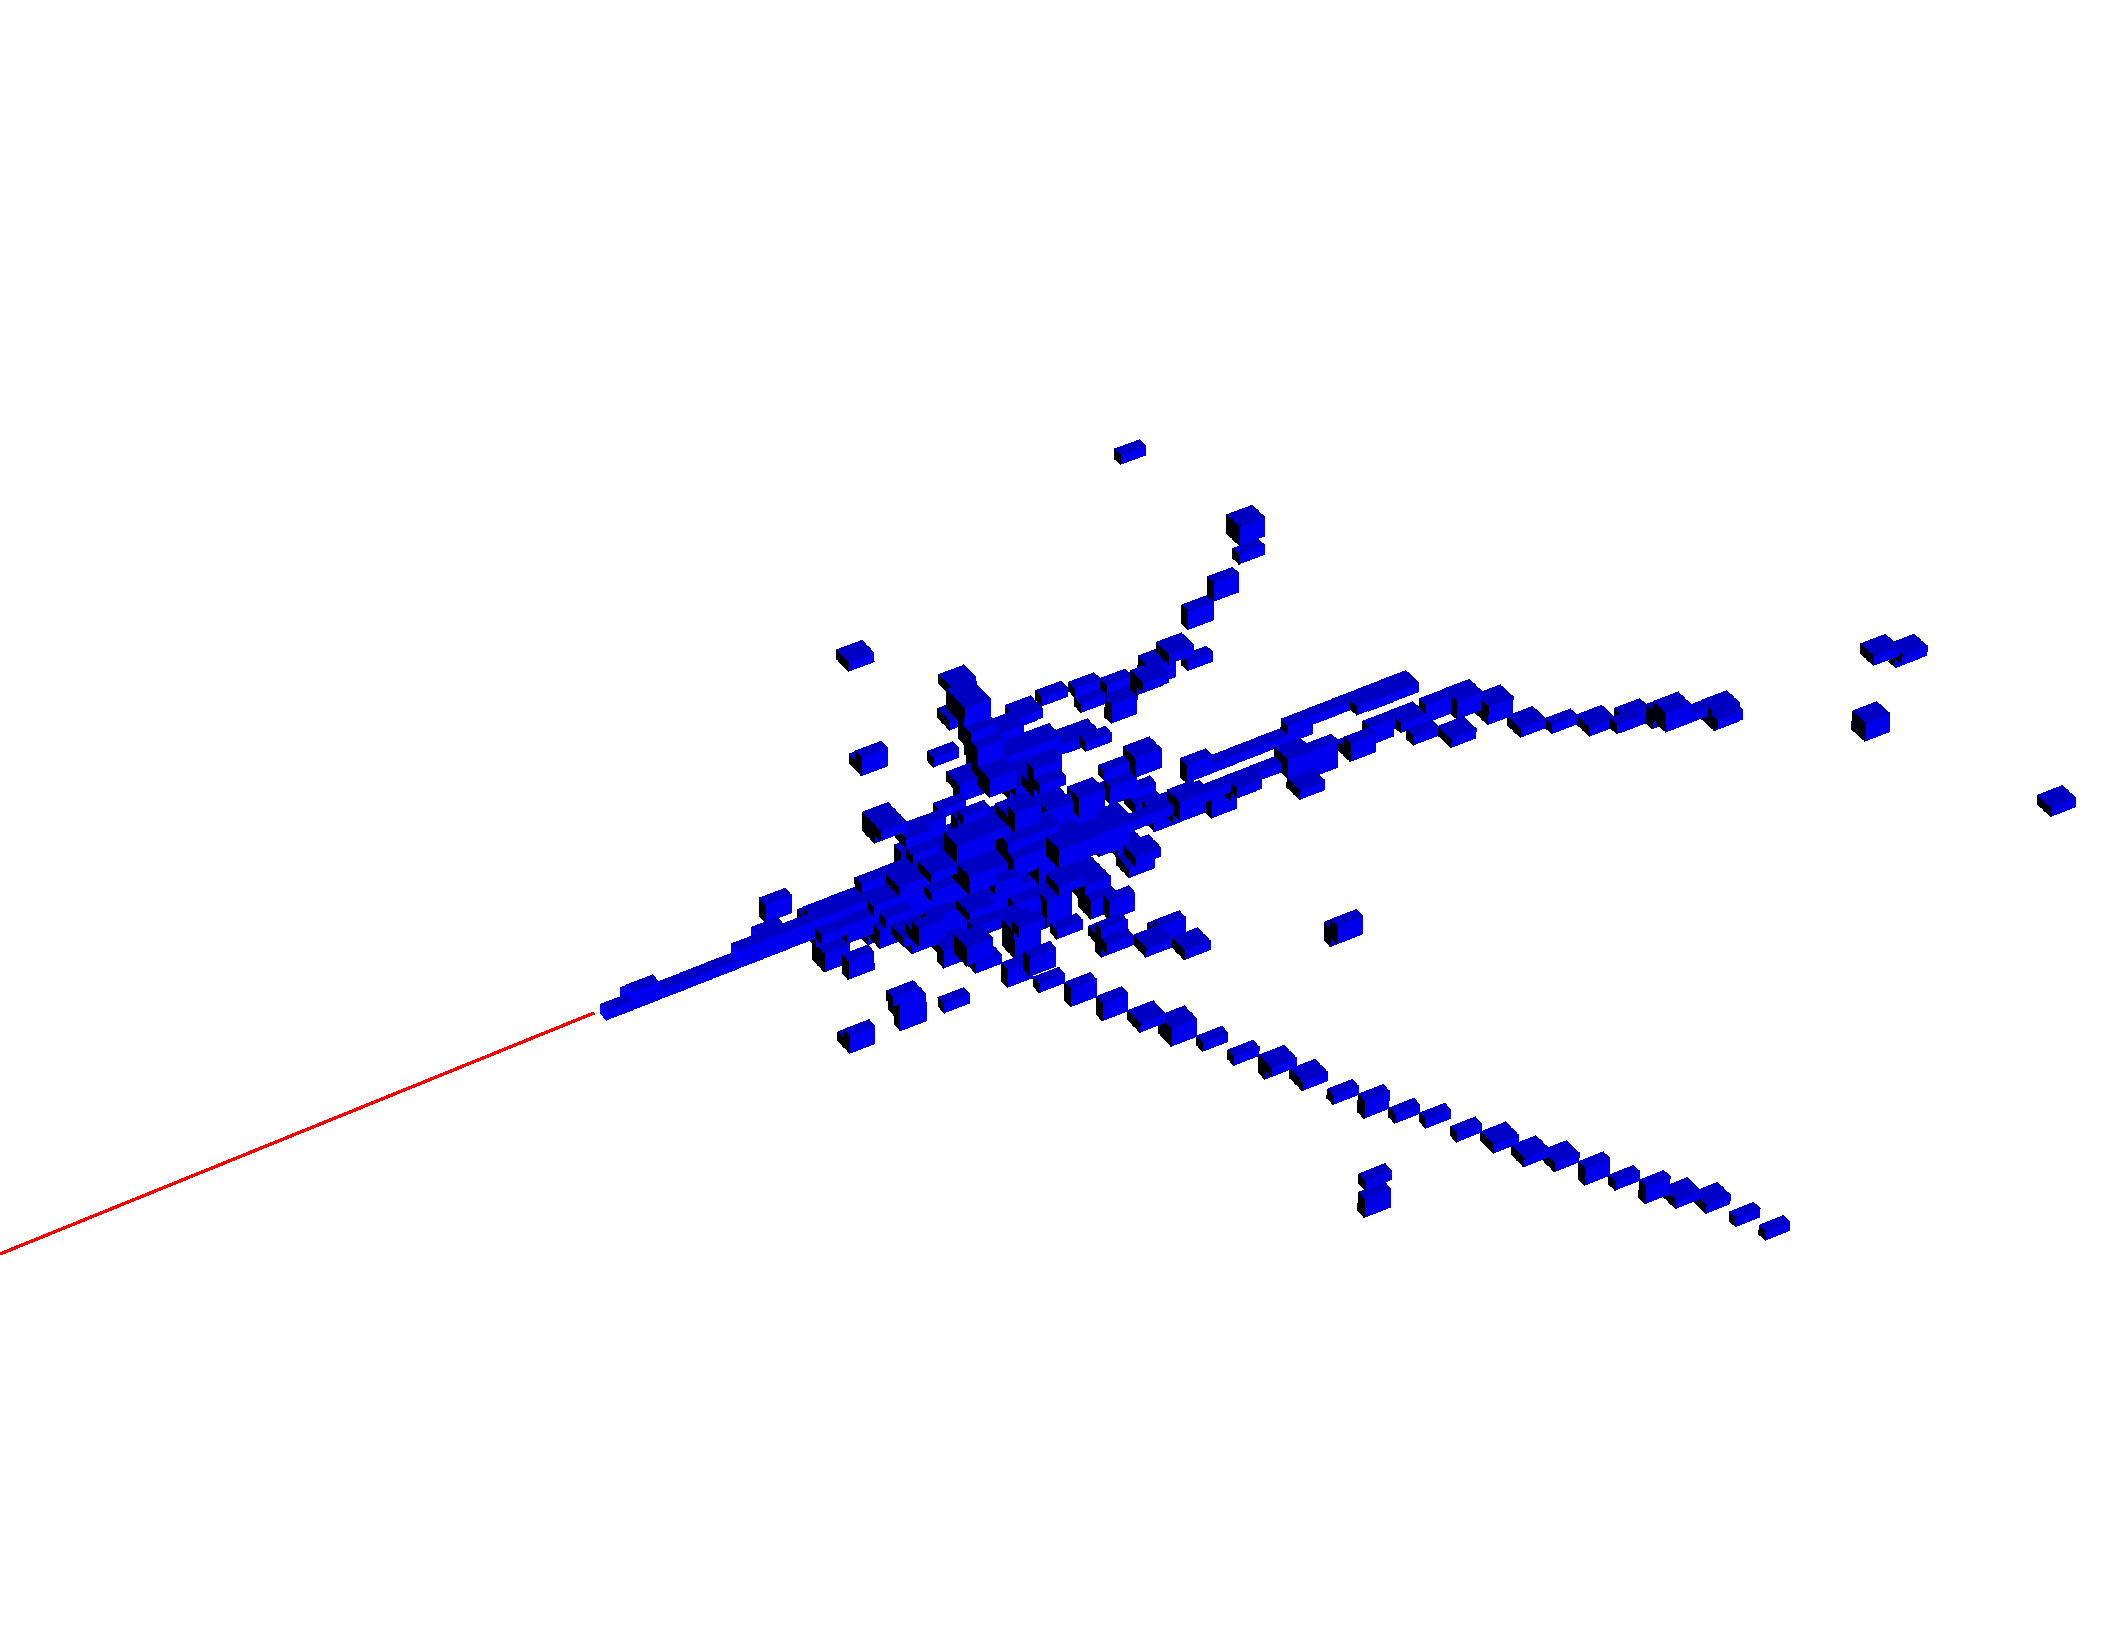
\includegraphics[width=0.9\linewidth]{SingleParticleSetup.pdf}      
      \end{center}
    \end{minipage}
  \end{frame}
  
  
  %% Performance ArborPFA - single particle - plots
  \begin{frame}
  \frametitle{Single particle analysis}
  \framesubtitle{Efficiency and Npfos}
    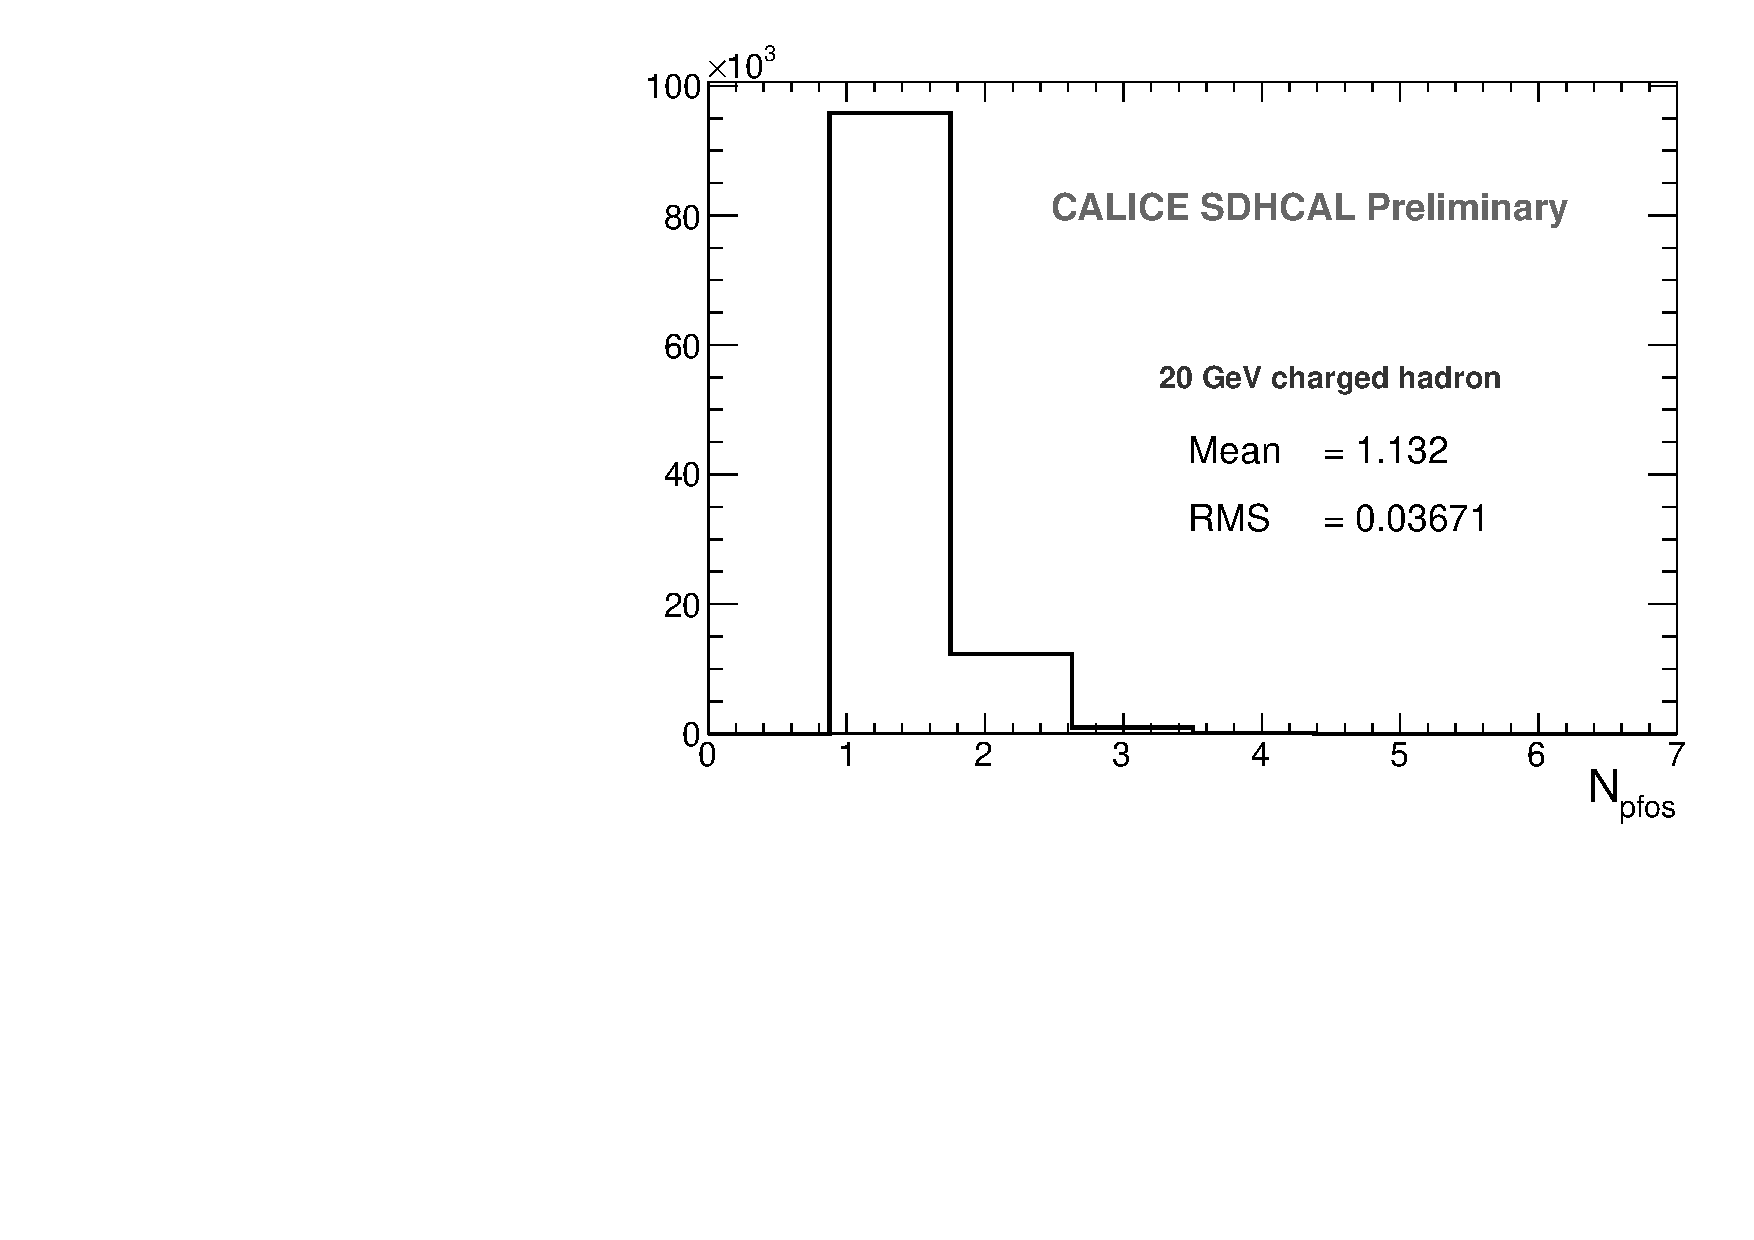
\includegraphics[width=0.45\linewidth]{SingleParticle_NPfos_20GeV.pdf}~
    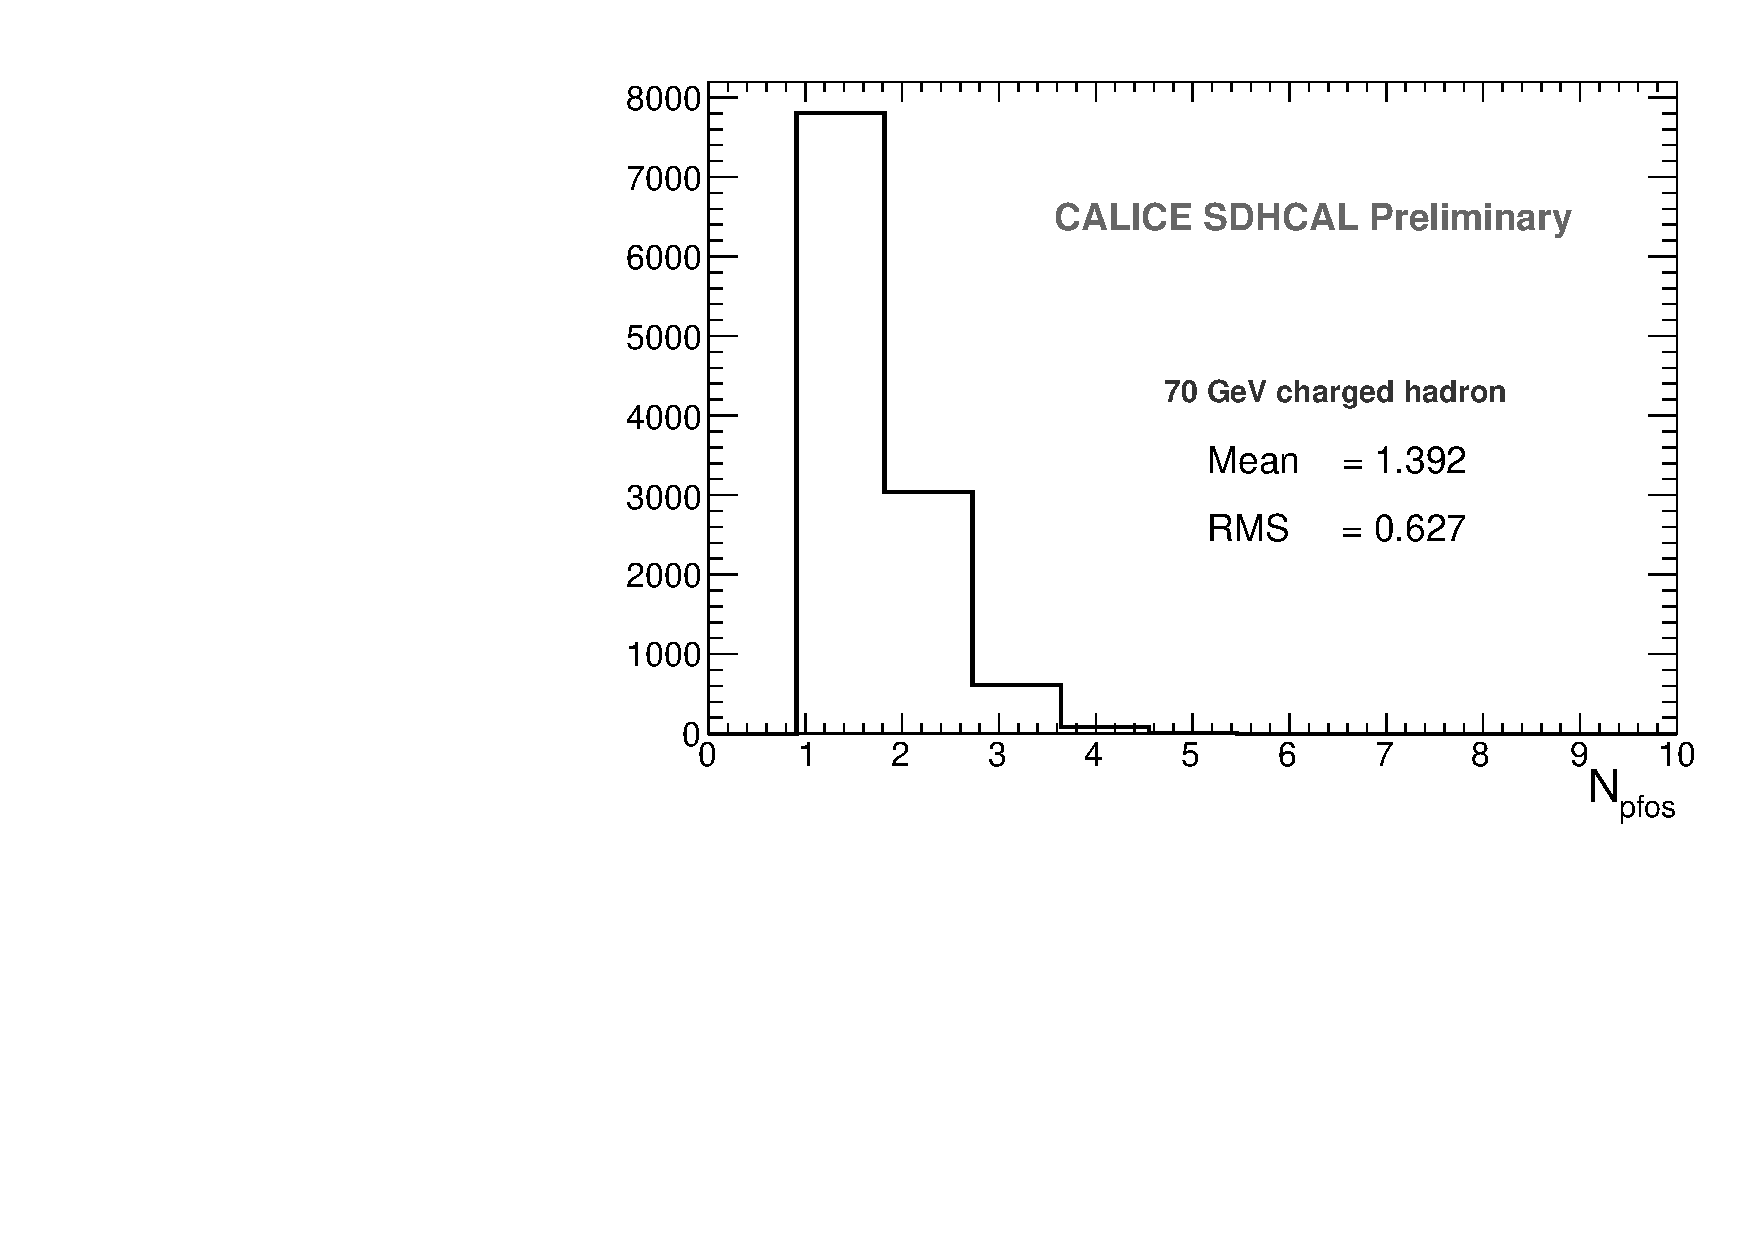
\includegraphics[width=0.45\linewidth]{SingleParticle_NPfos_70GeV.pdf} \\
    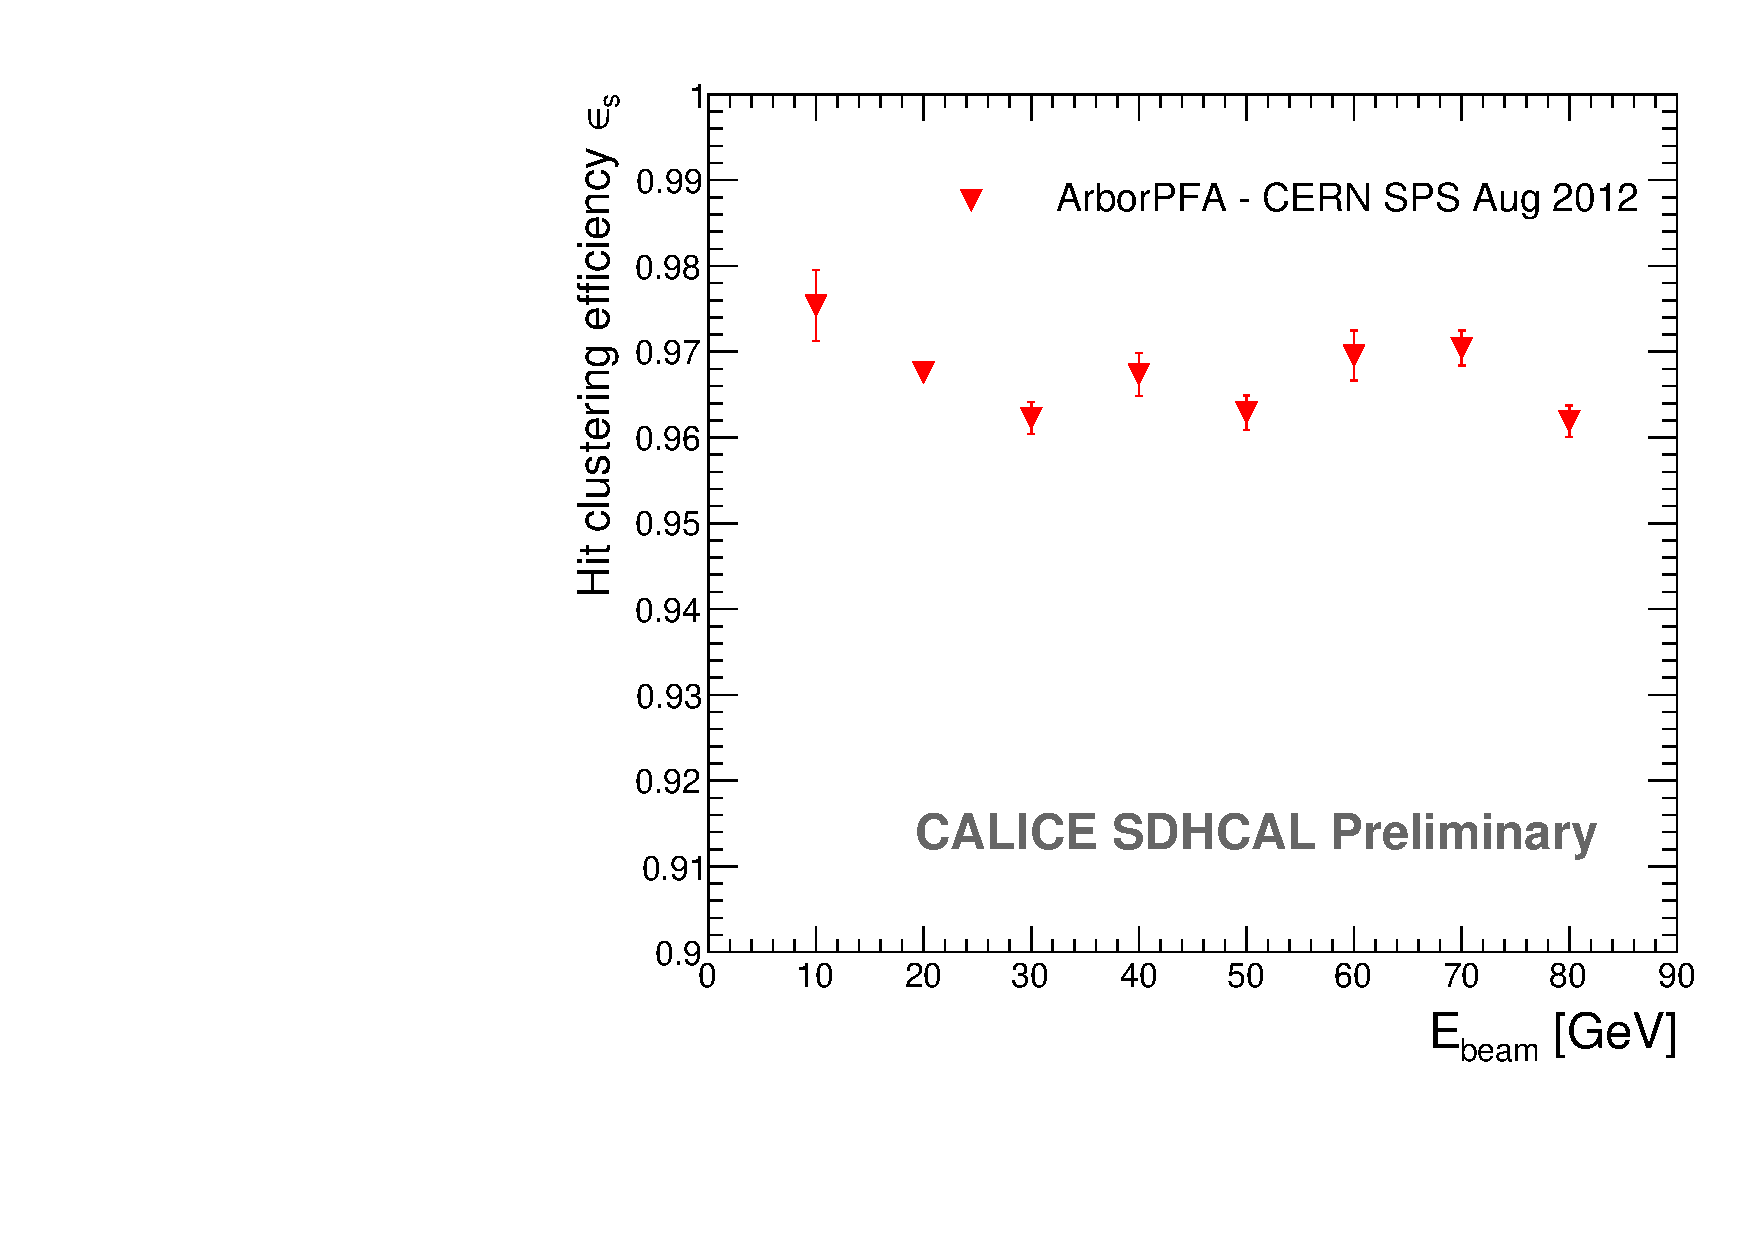
\includegraphics[width=0.45\linewidth]{SingleParticle_Efficiency.pdf}~
    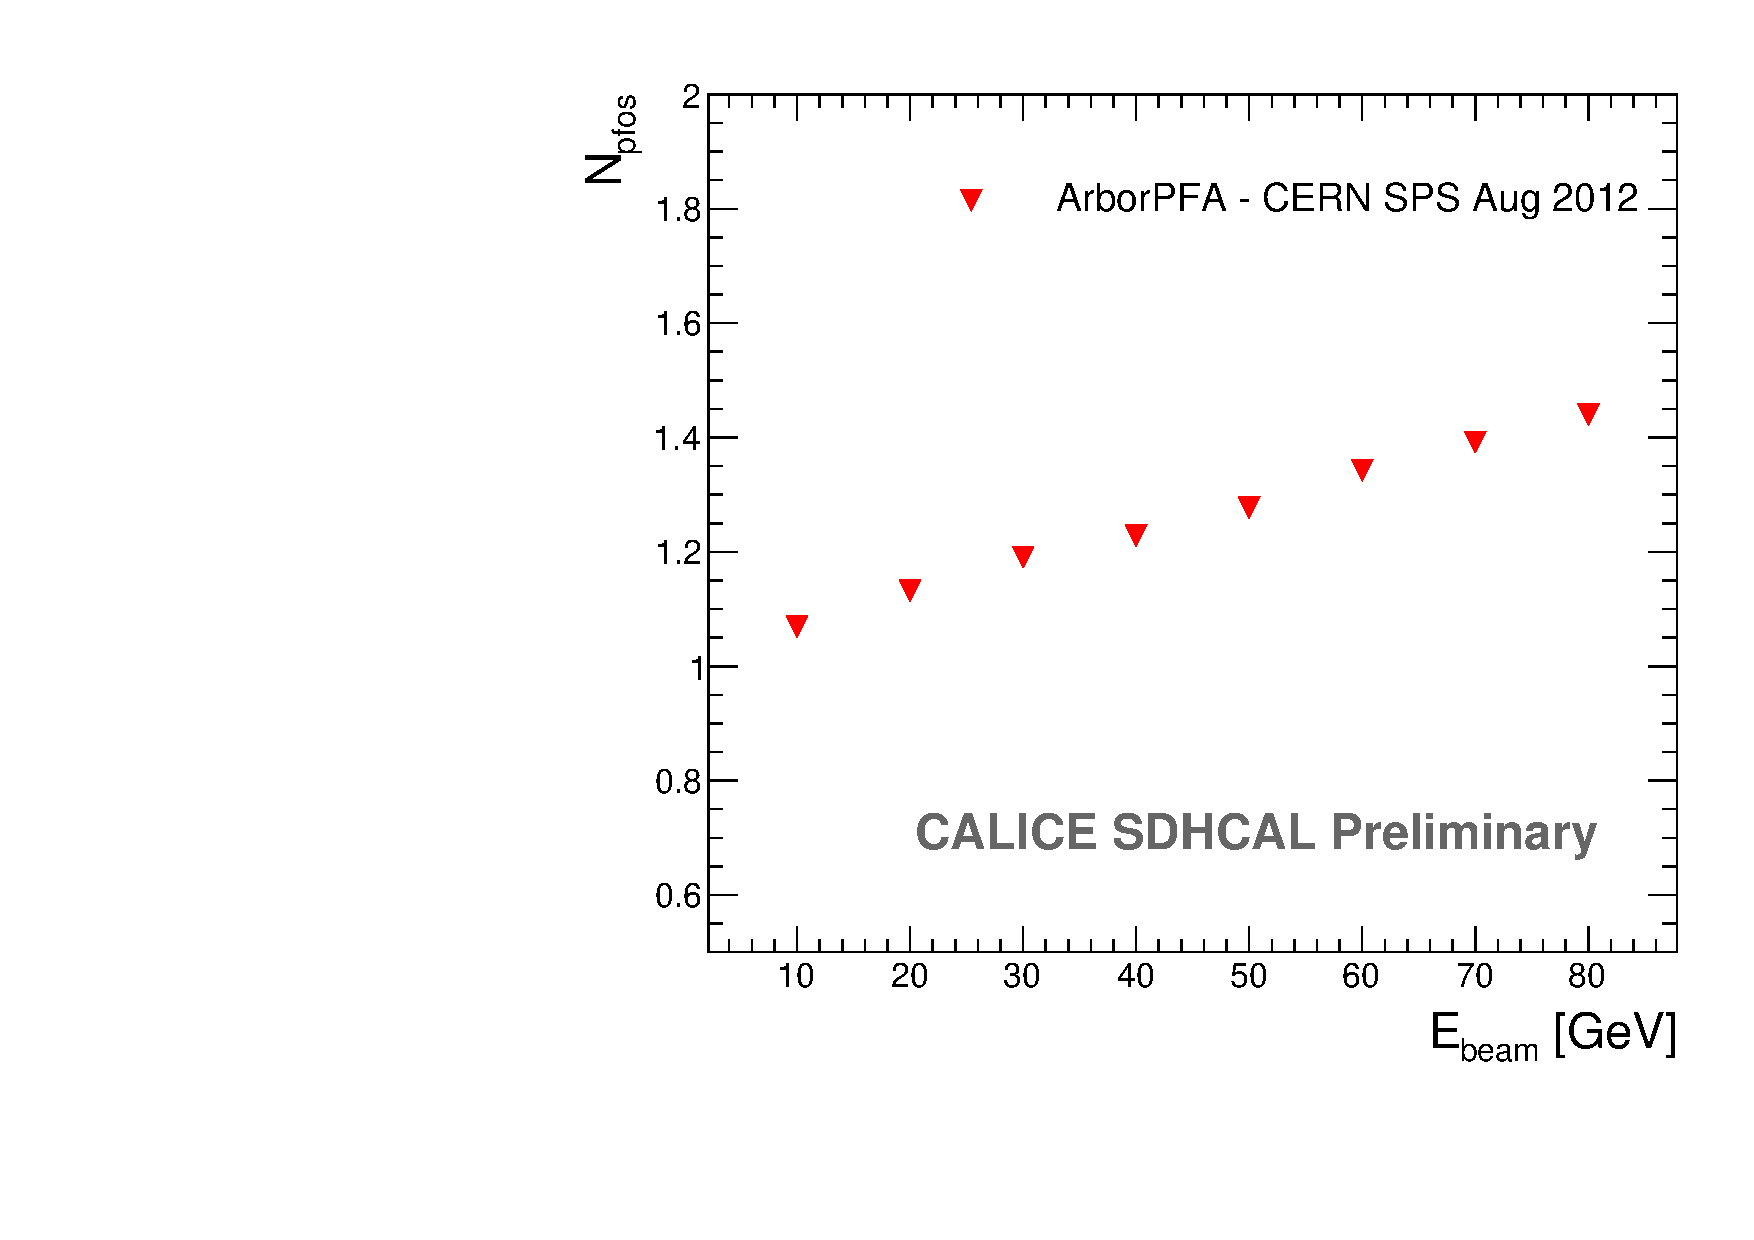
\includegraphics[width=0.45\linewidth]{SingleParticle_NPfos.pdf}
  \end{frame}
  
  %% Performance ArborPFA - single particle - plots
  \begin{frame}
  \frametitle{Single particle analysis}
  \framesubtitle{Reconstructed energy and resolution}
    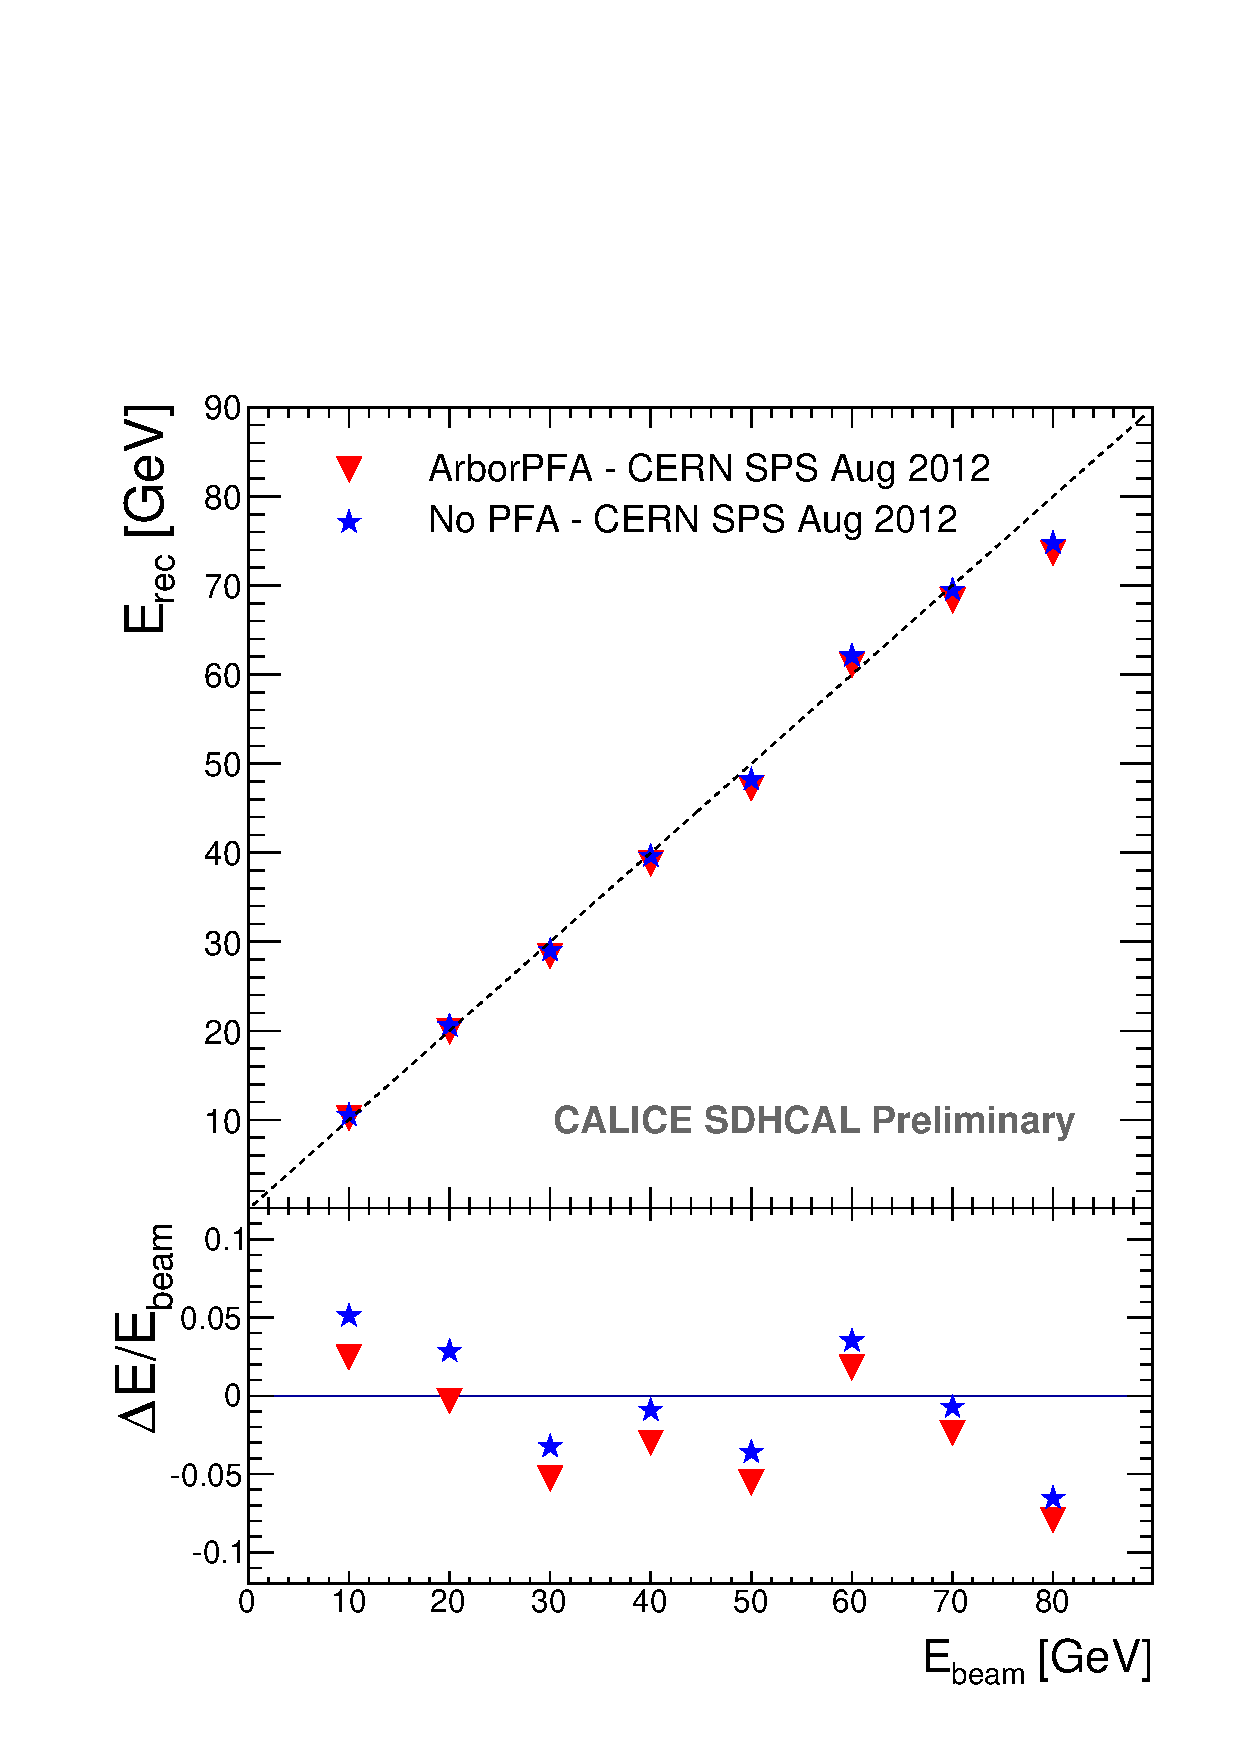
\includegraphics[width=0.45\linewidth]{SingleParticle_ERec.pdf}~
    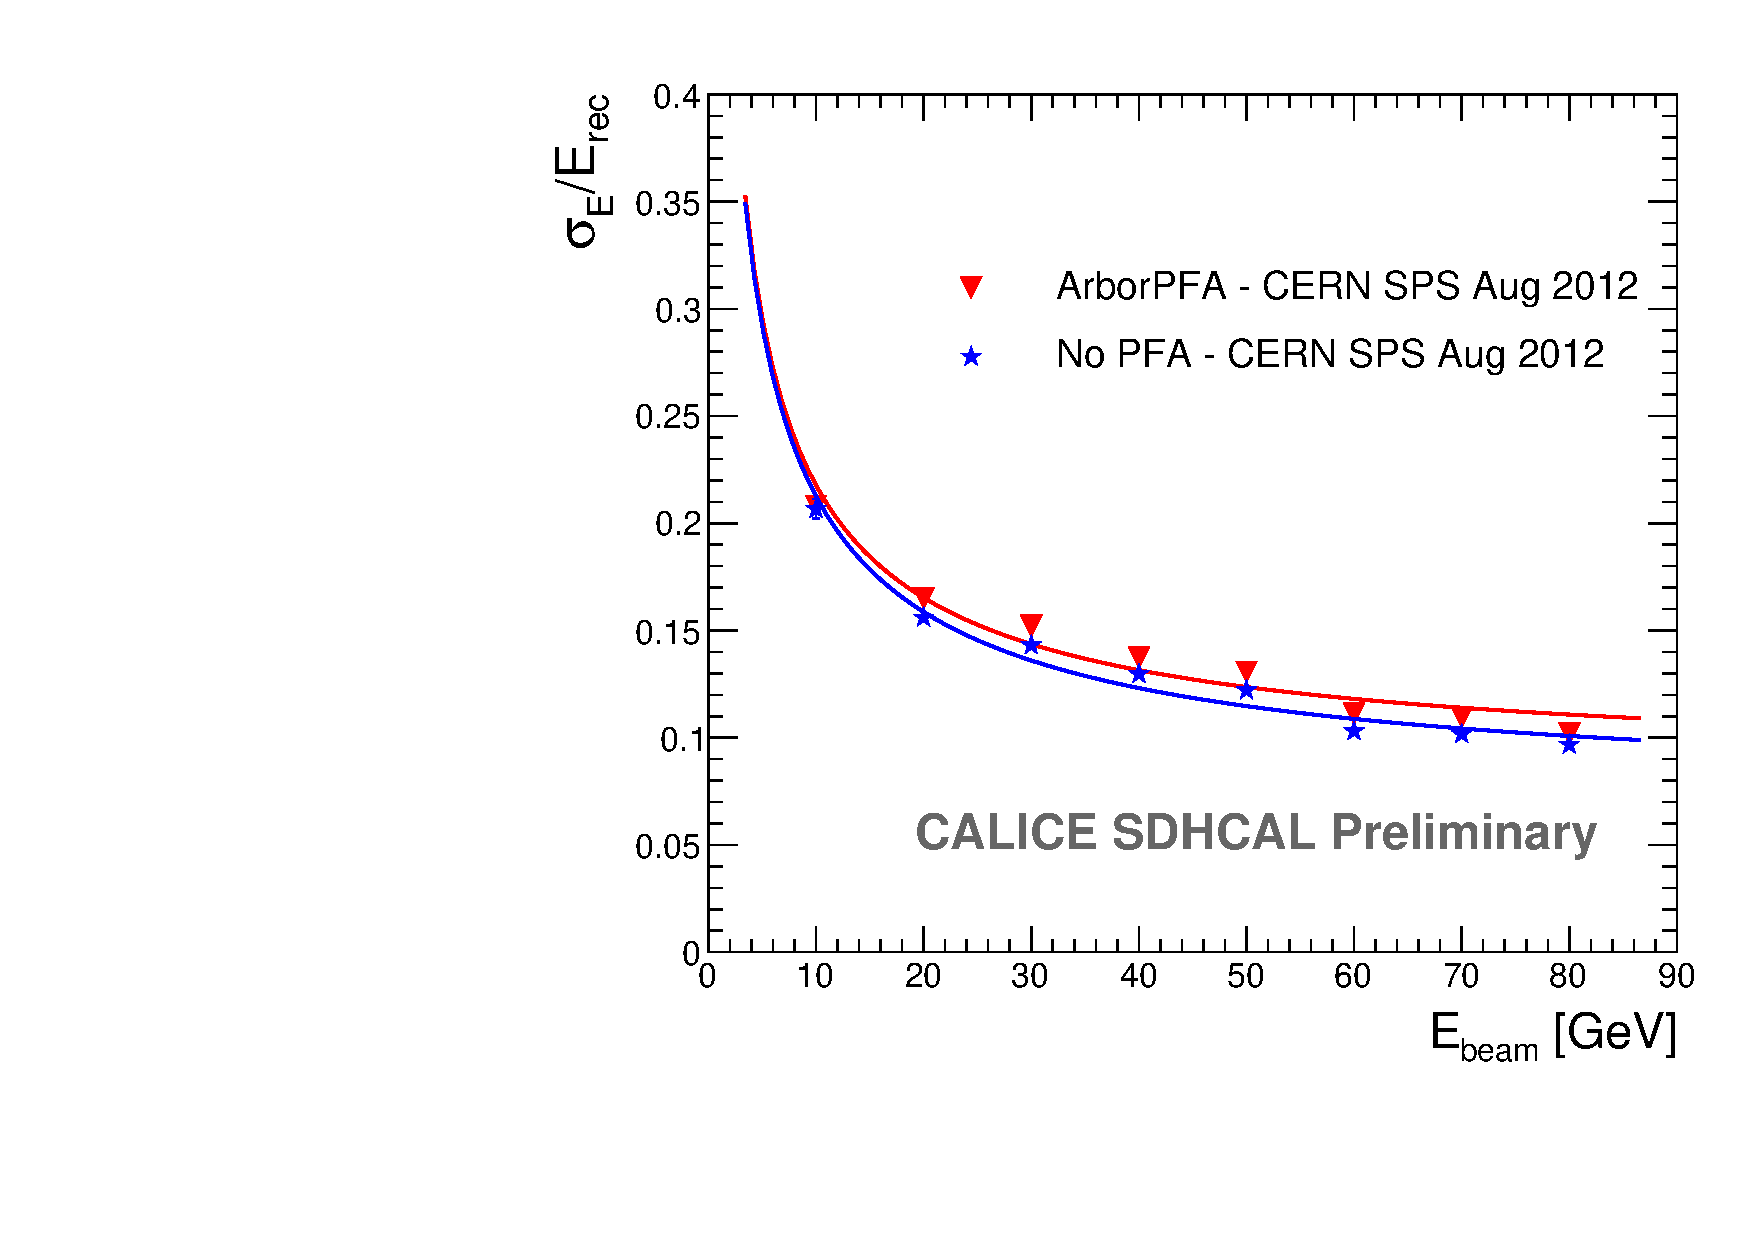
\includegraphics[width=0.45\linewidth]{SingleParticle_EResol.pdf}
  \end{frame}
  
  
%  \subsection{Performance - Deux hadrons superposés}
  \subsection{Overlaid particle performances}
  \begin{frame}
  \frametitle{Overlaid particles}
  %\framesubtitle{\subsecname}
    \begin{block}{Overlay of two hadronic events}
      \begin{itemize}
        \item Same data set
        \item Particle 1 energy : 10 GeV
        \item Particle 2 energies : [10 ; 50] GeV by steps of 10 GeV
      \end{itemize}
      Overlay algorithm :
      \begin{itemize}
        \item Determination of entry points and barycentres.
        \item Removal of hits belonging to the primary track segment of particle 1 (10 GeV)
        \item Shower re-centered in calorimeter (x and y) and $\pm$ d/2 shift in the x direction
        \item Overlaid hits : the highest threshold is kept
        \item Hits are tagged 1, 2 or 3 (overlaid)
      \end{itemize}
    \end{block}
    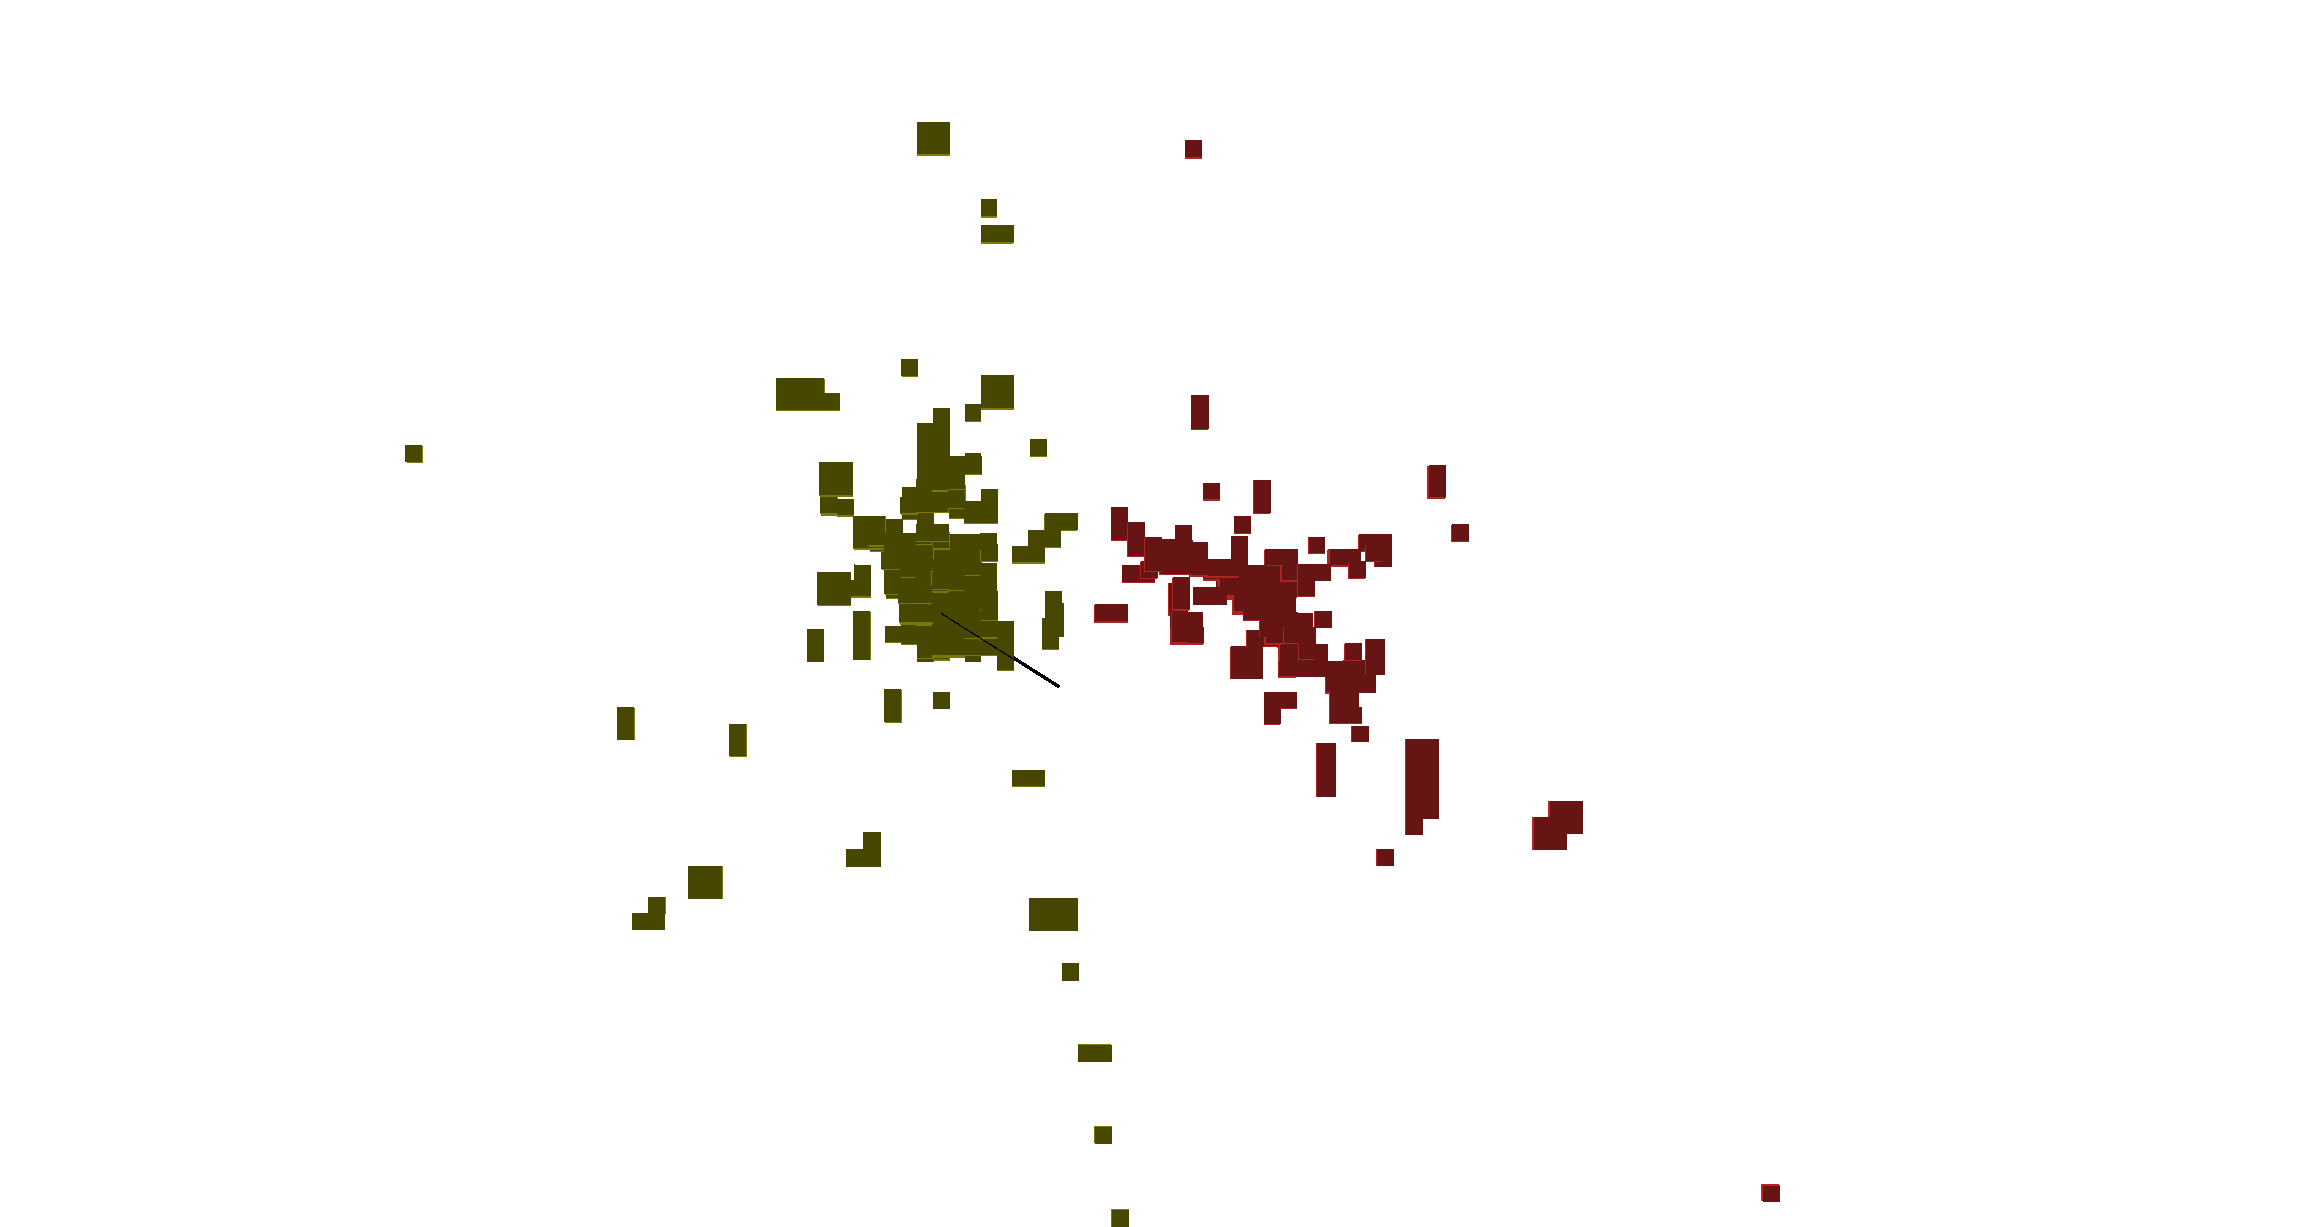
\includegraphics[width=0.32\linewidth]{ArborPFA_PandoraMonitoring_SDHCAL_Overlay_XY.pdf}
    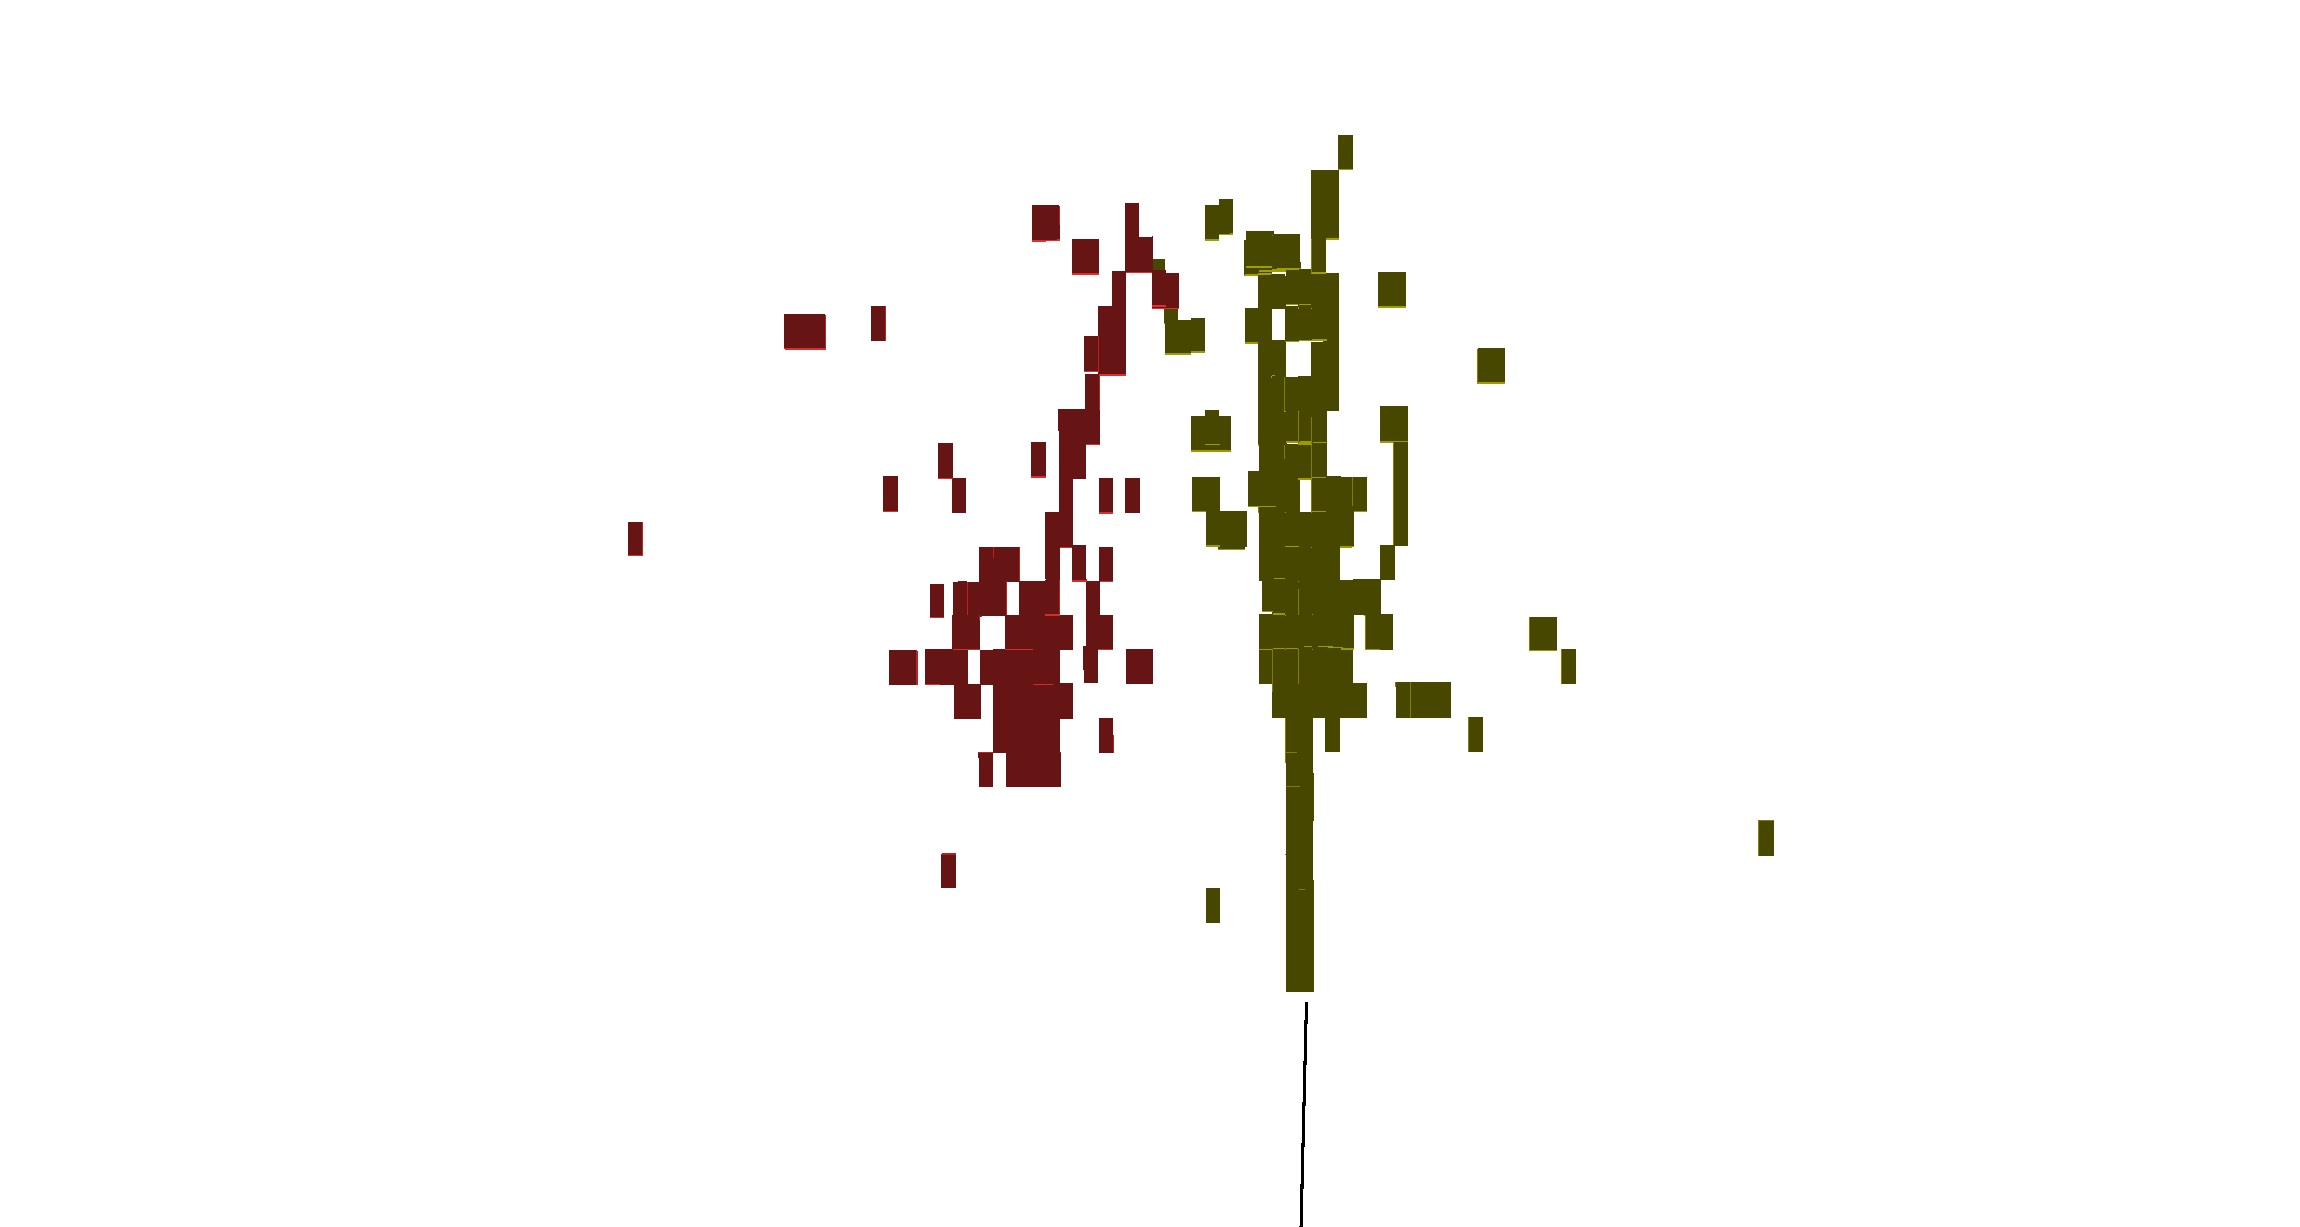
\includegraphics[width=0.32\linewidth]{ArborPFA_PandoraMonitoring_SDHCAL_Overlay_XZ.pdf}
    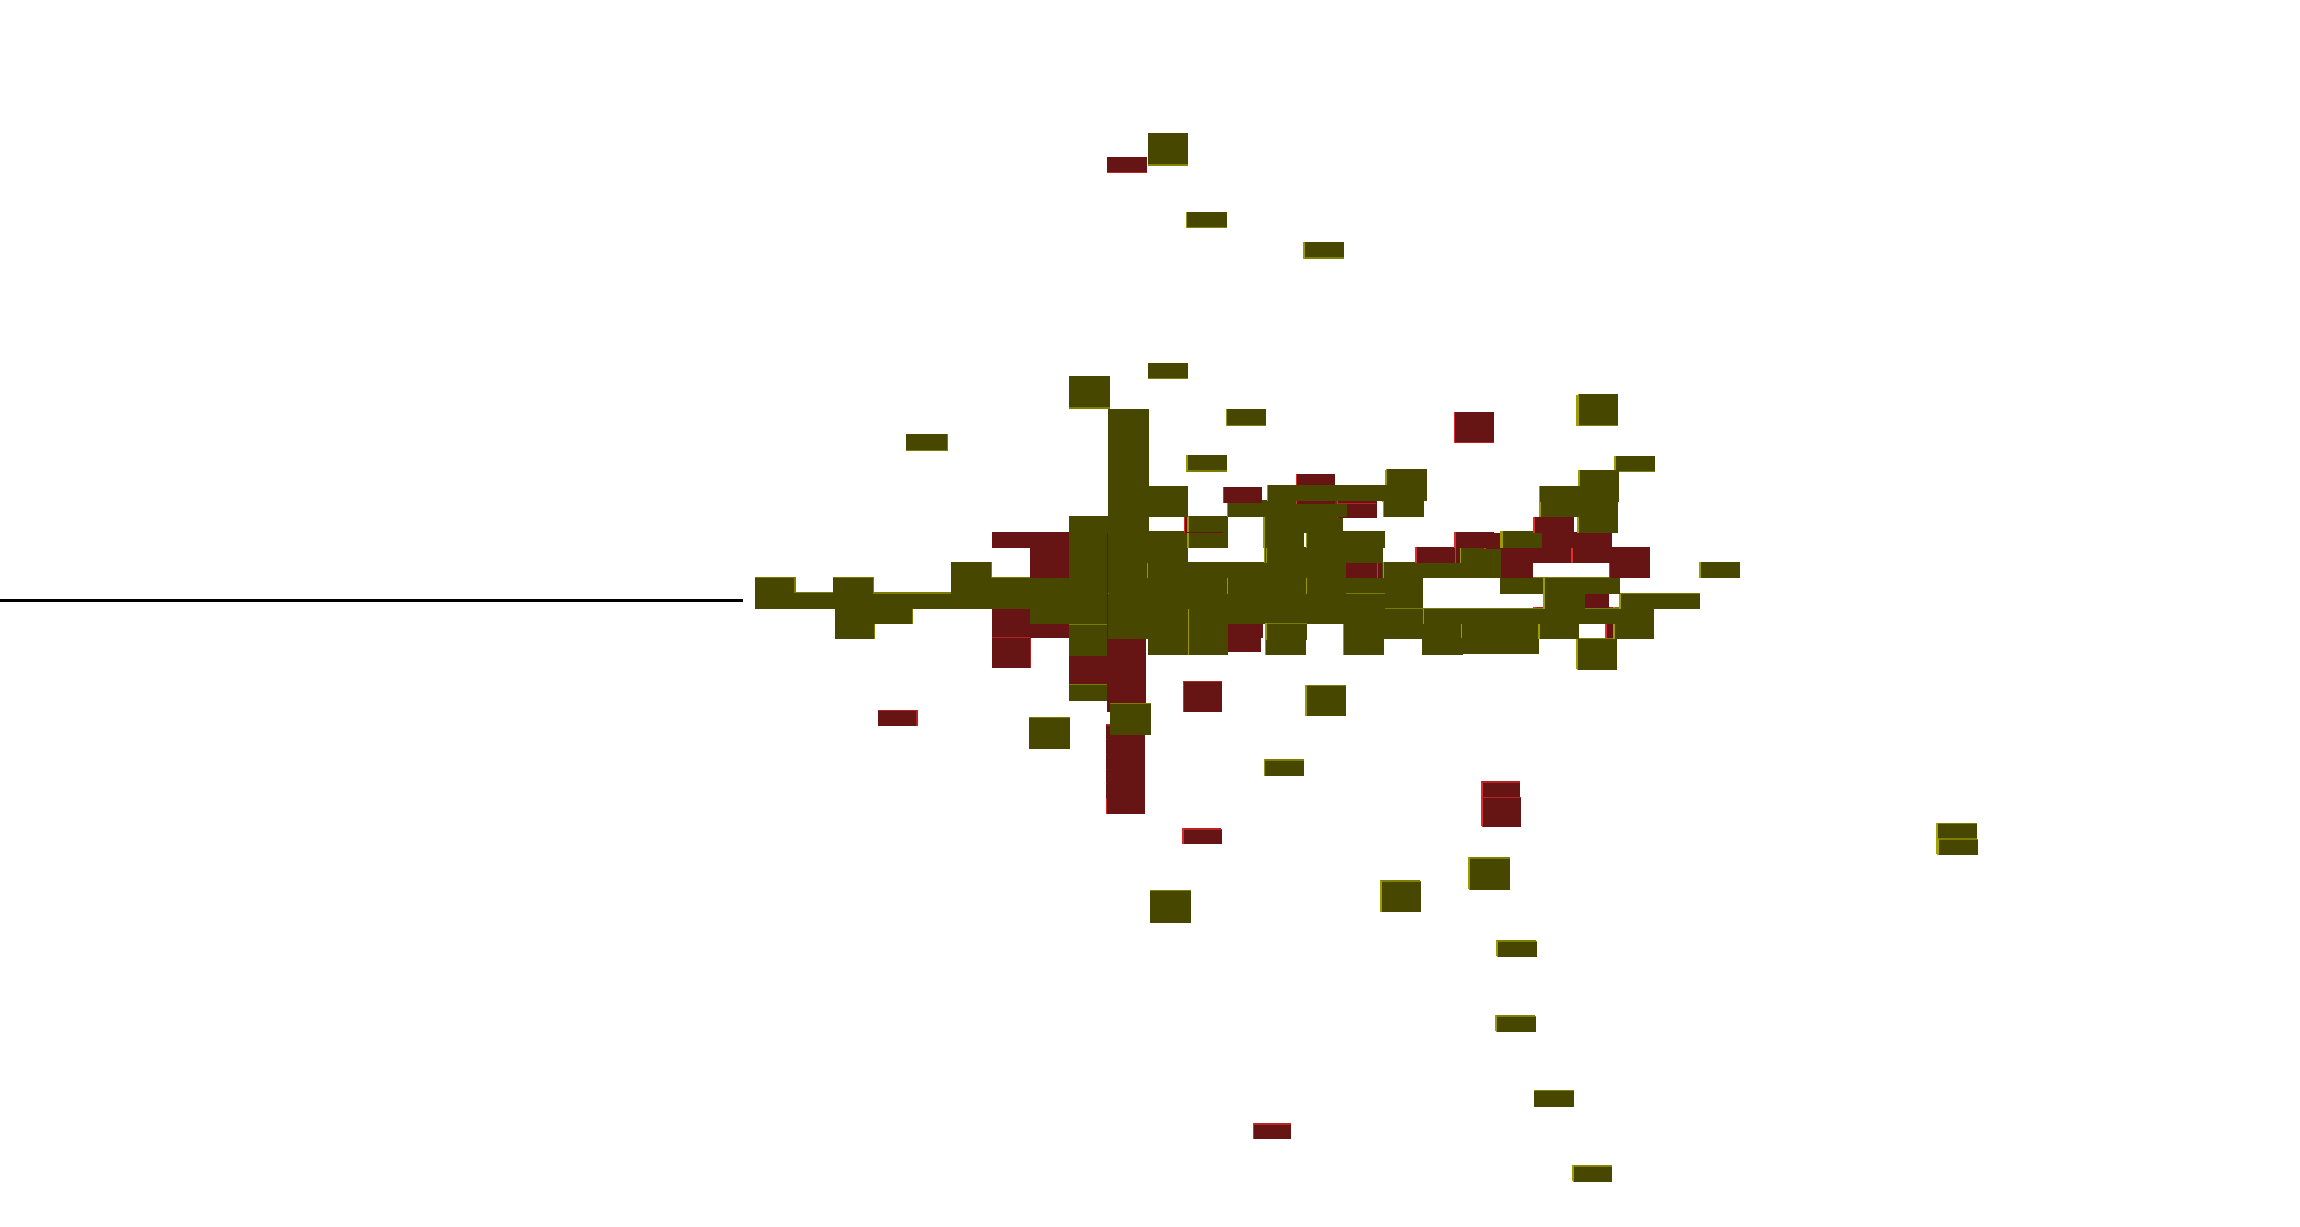
\includegraphics[width=0.32\linewidth]{ArborPFA_PandoraMonitoring_SDHCAL_Overlay_YZ.pdf}
  \end{frame}
  
 
  %% Overlay event - plots 2
  \begin{frame}
  \frametitle{Overlaid particles}
  \framesubtitle{Efficiency and purity}
    
    \begin{minipage}{0.49\linewidth}
      \begin{center}
        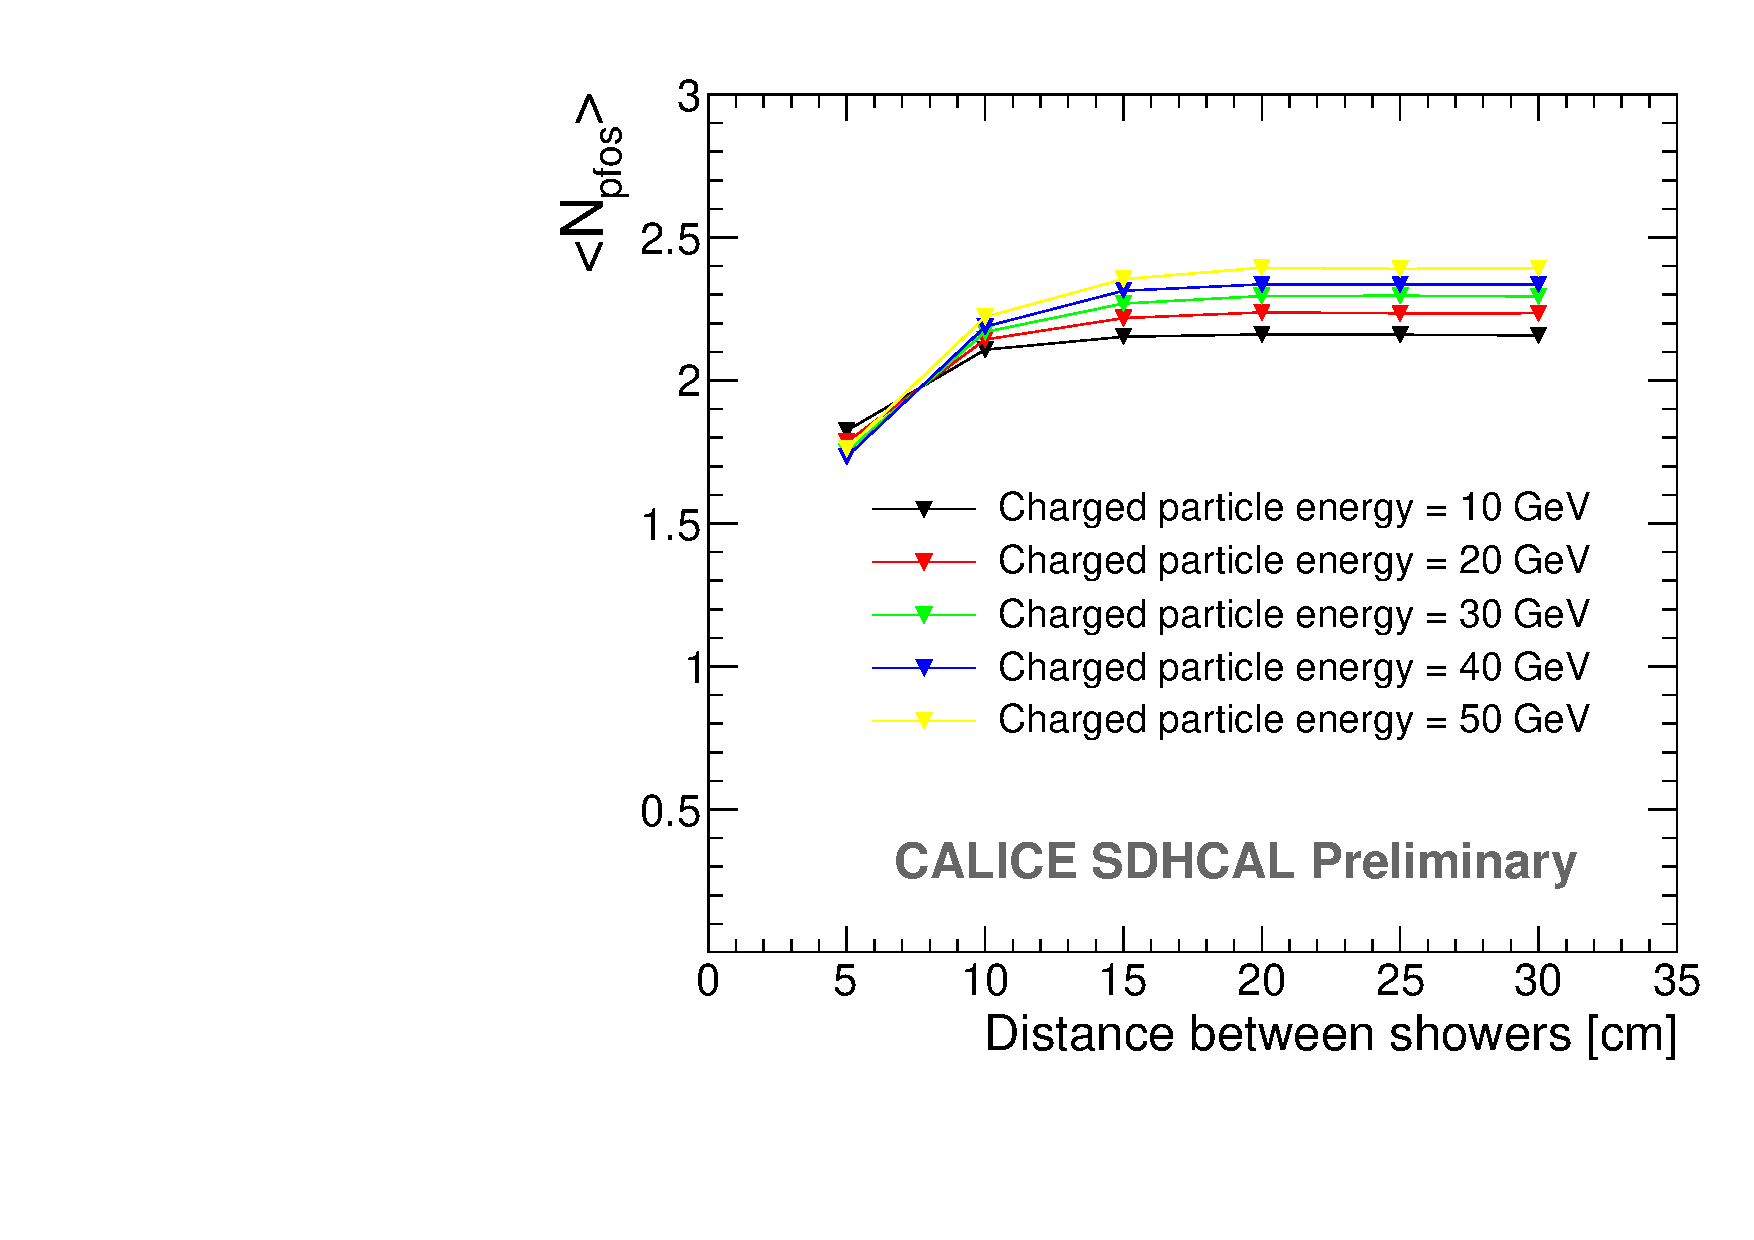
\includegraphics[width=0.8\linewidth]{OverlayEvent_NPfos.pdf}     
      \end{center}
    \end{minipage} \hfill
    \begin{minipage}{0.49\linewidth}
      \begin{block}{Efficiency and purity}
        \begin{equation}
          \epsilon = \frac{Nhit_{good}}{Nhit_{ini,tot}}
        \end{equation}
        \begin{equation}
          \rho = \frac{Nhit_{good}}{Nhit_{rec,tot}}
        \end{equation}
      \end{block}
    \end{minipage}
    \begin{center}
      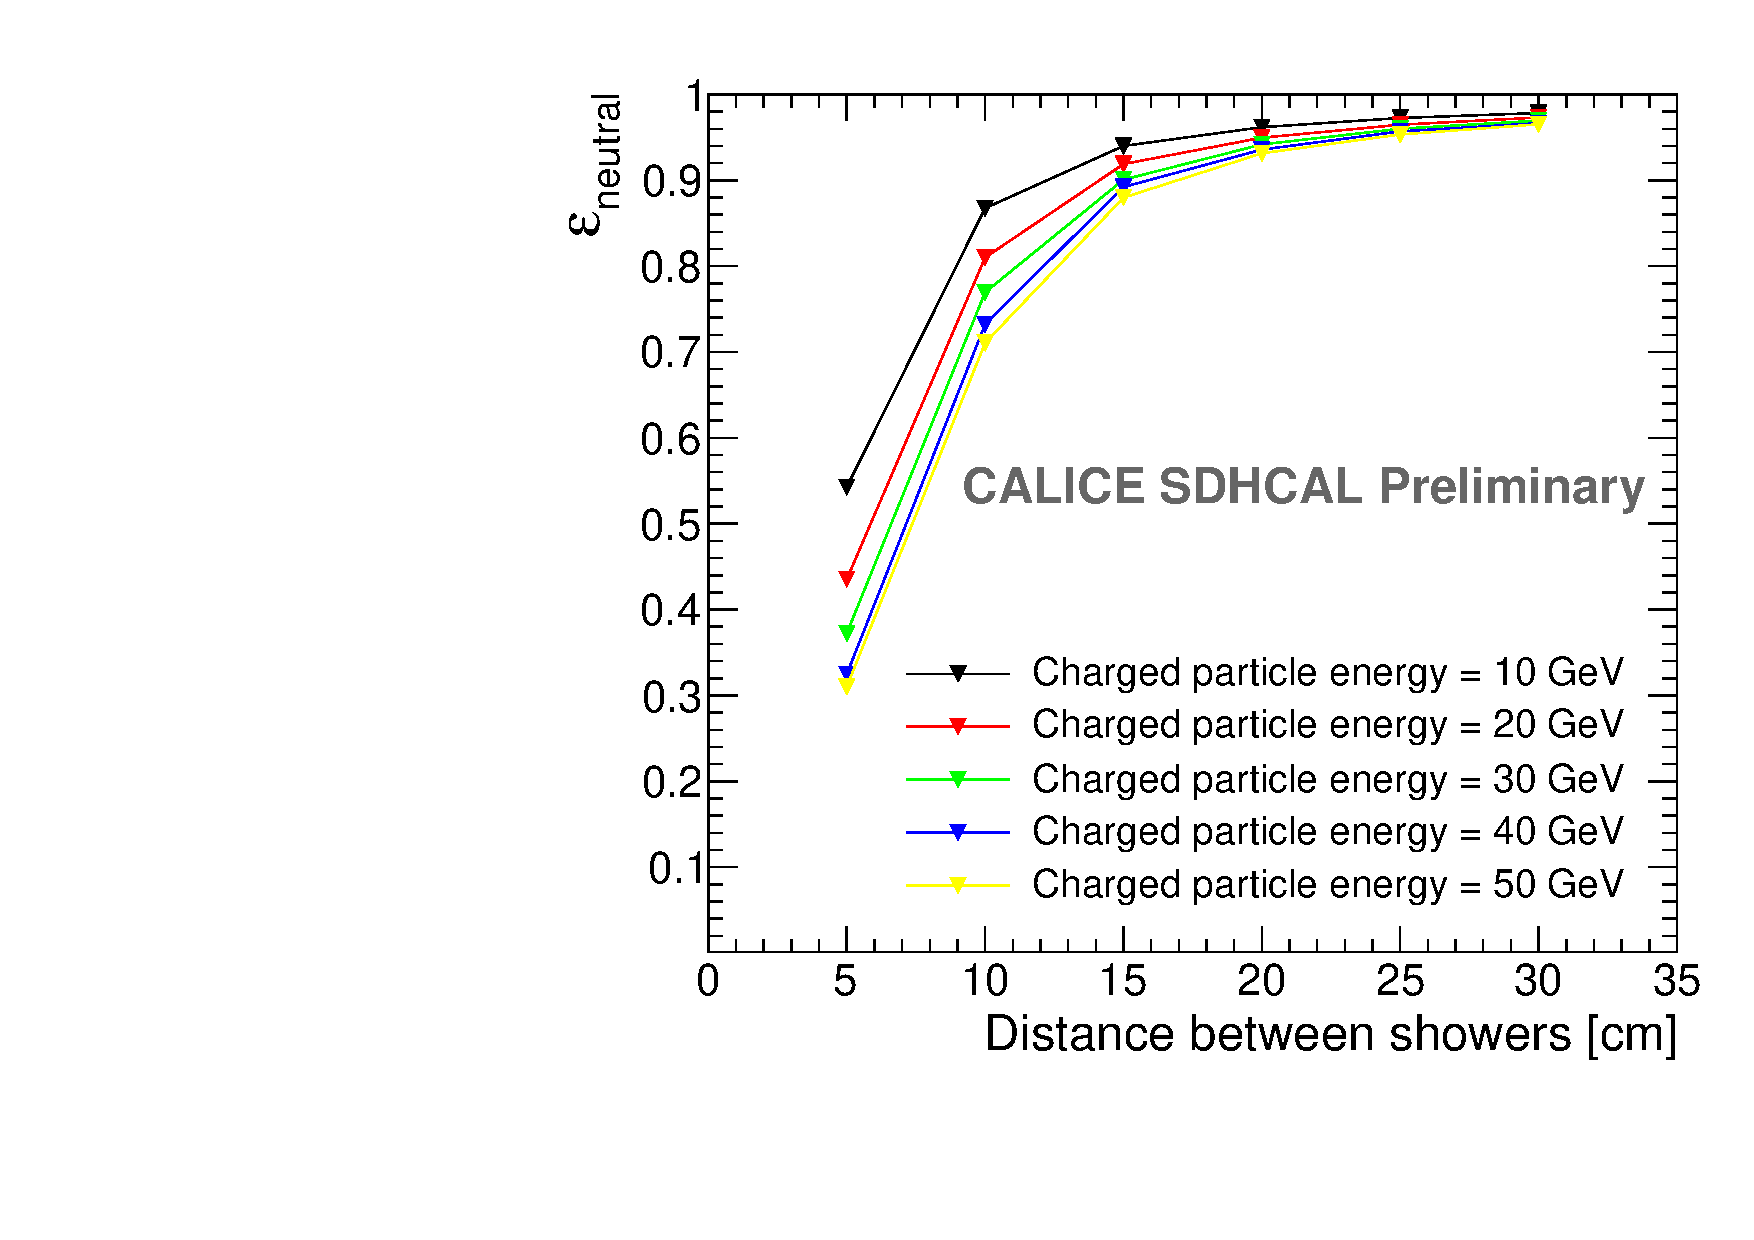
\includegraphics[width=0.4\linewidth]{OverlayEvent_NeutralEfficiency.pdf} ~~~~~~~~~~~~~~~~
      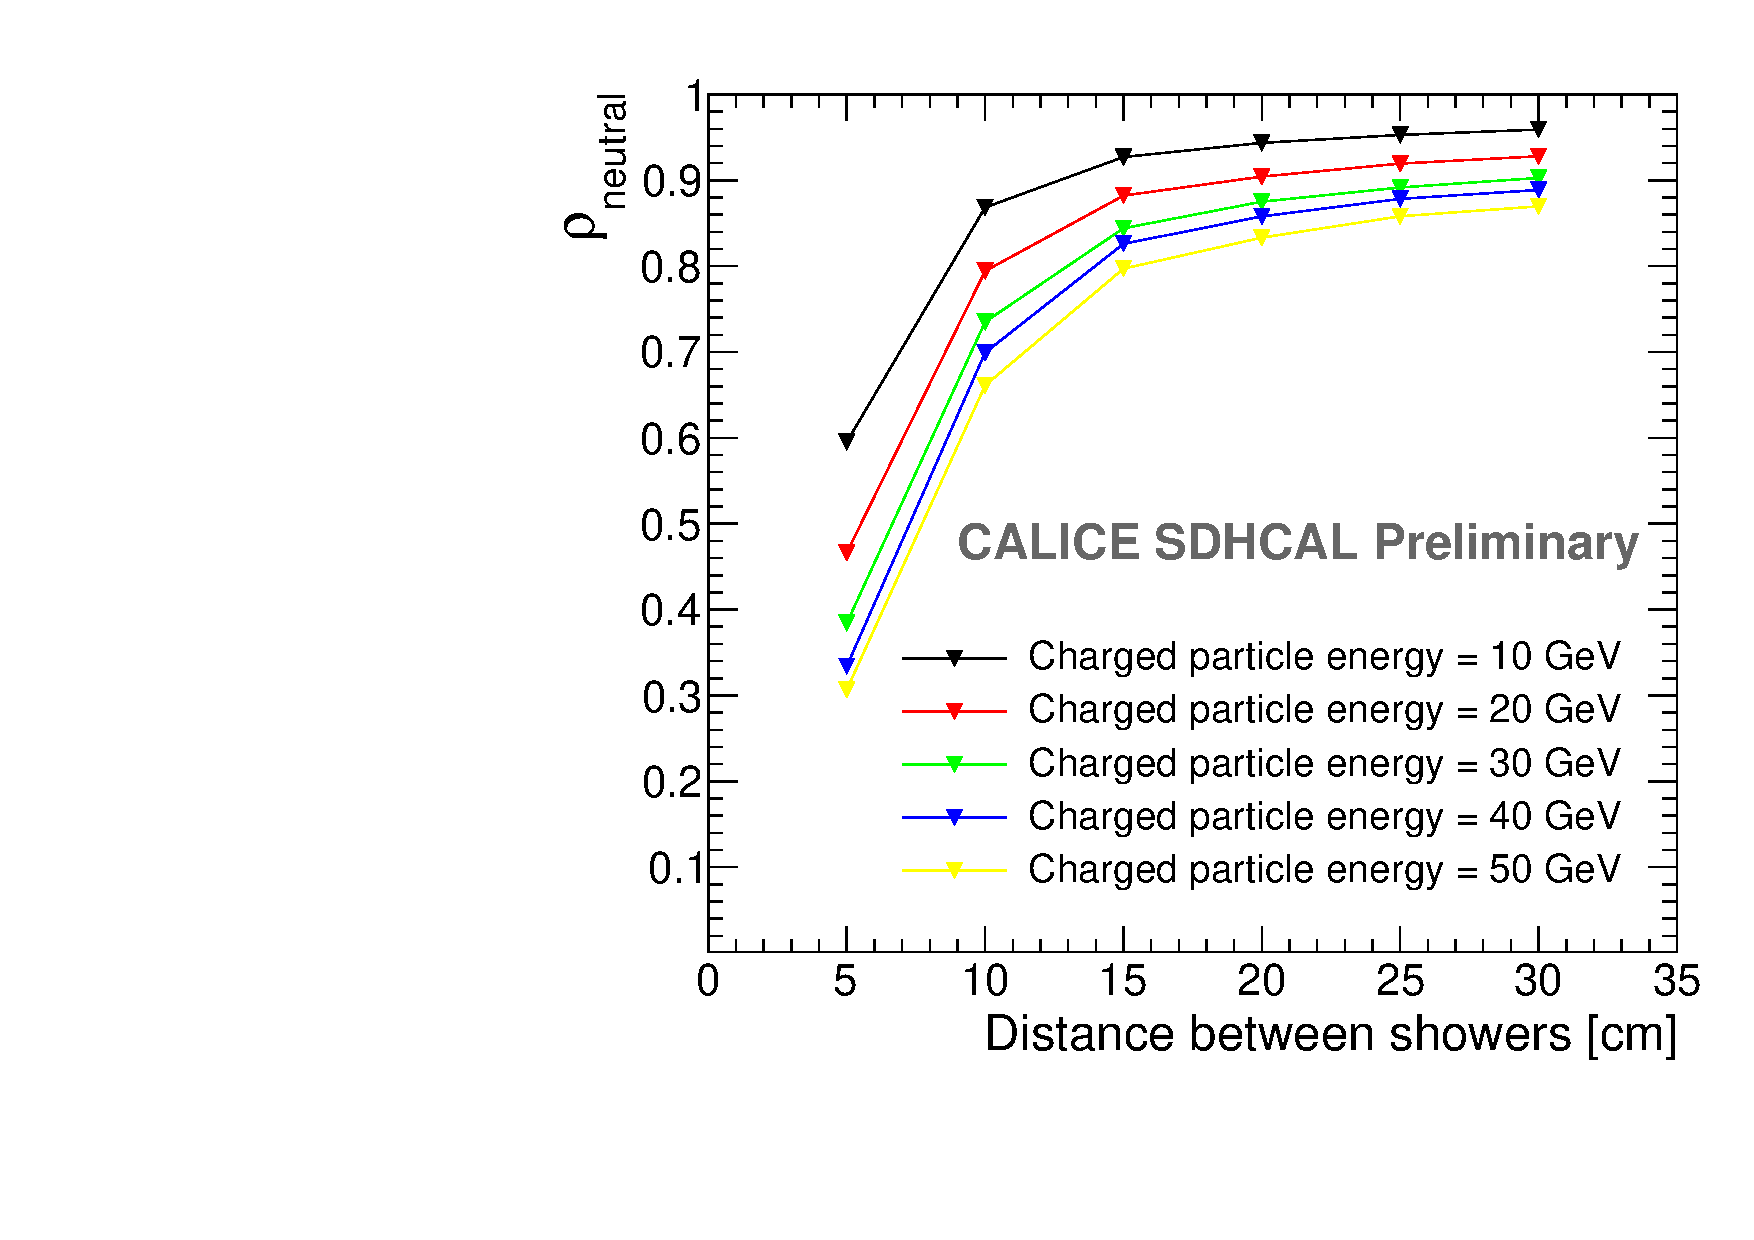
\includegraphics[width=0.4\linewidth]{OverlayEvent_NeutralPurity.pdf}     
    \end{center}
  \end{frame}


  %% Overlay event - plots 3
  \begin{frame}
  \frametitle{Overlaid particles}
  \framesubtitle{Probability and energy}
    \begin{center}
      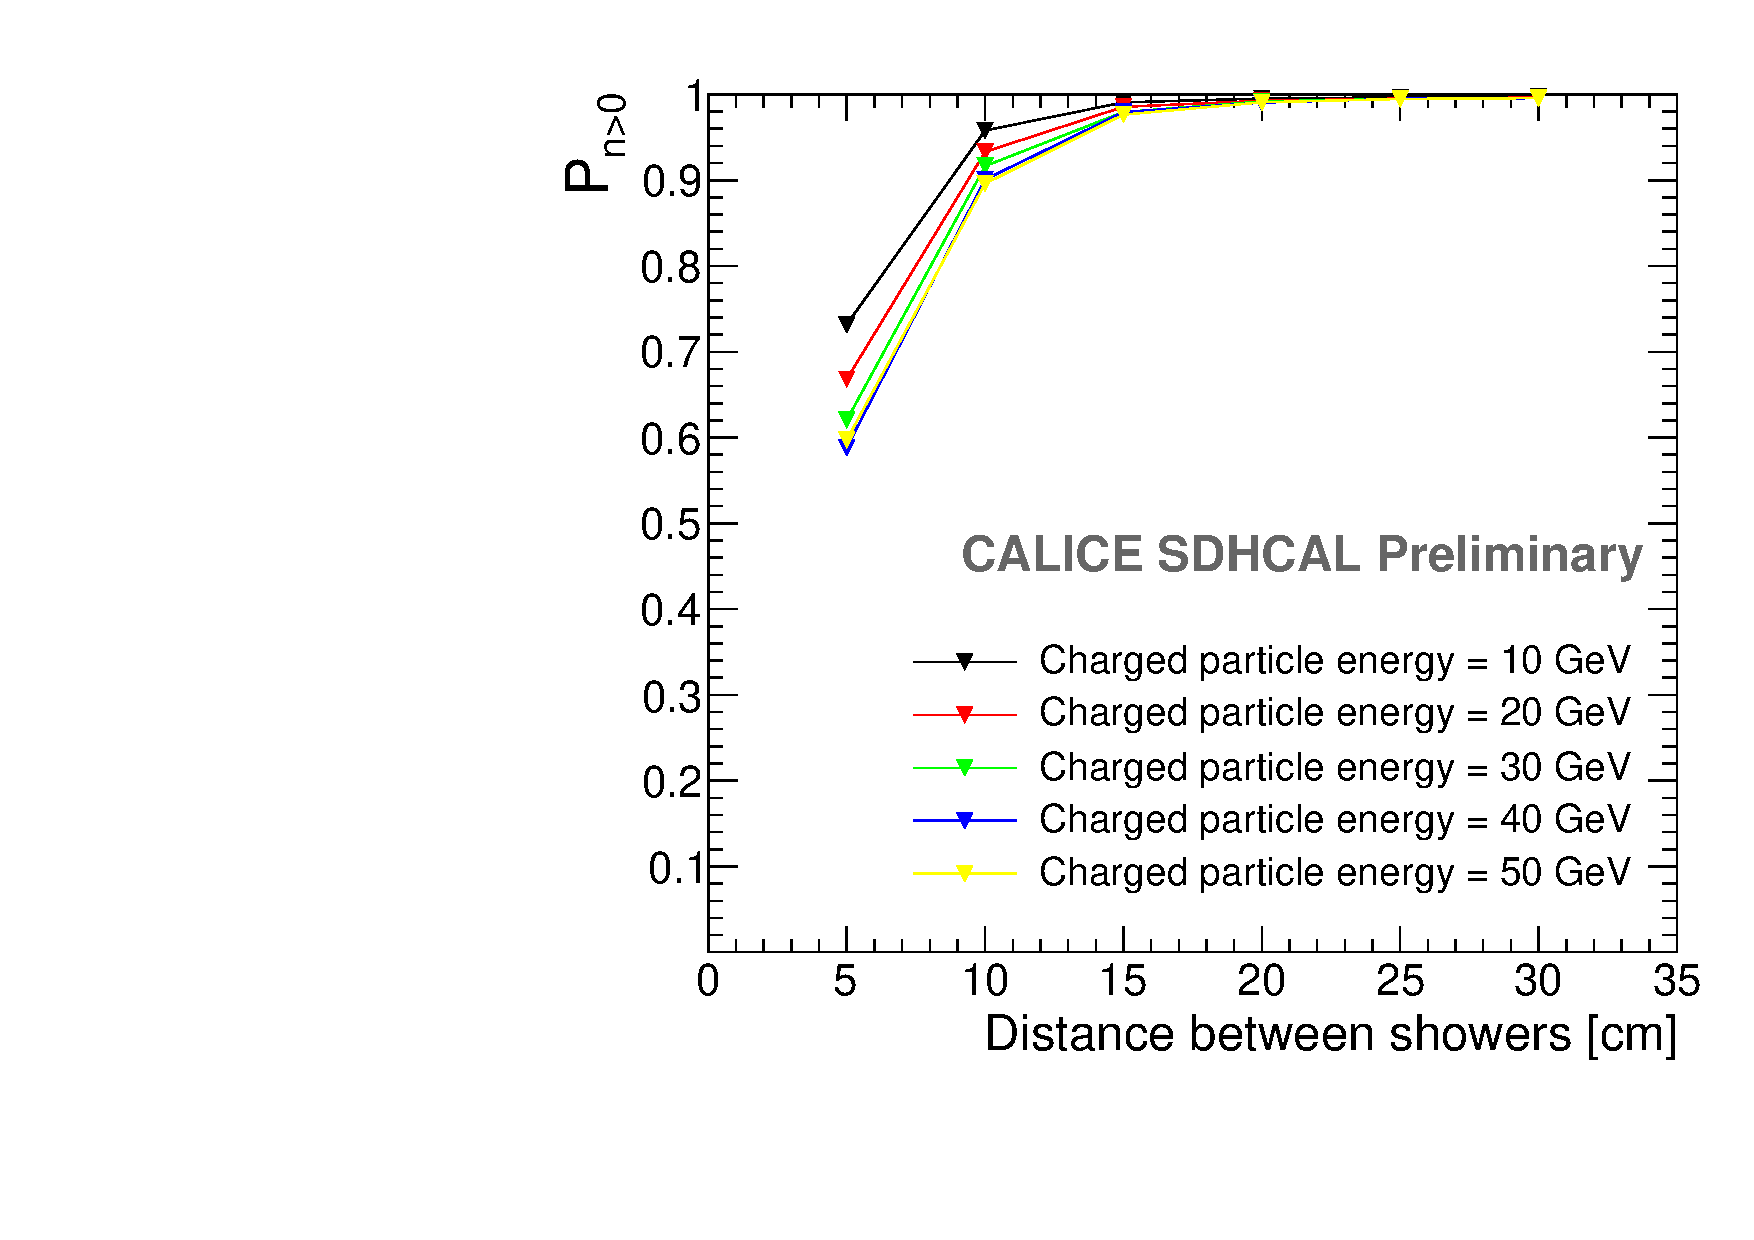
\includegraphics[width=0.48\linewidth]{OverlayEvent_NeutralPercentage.pdf}
      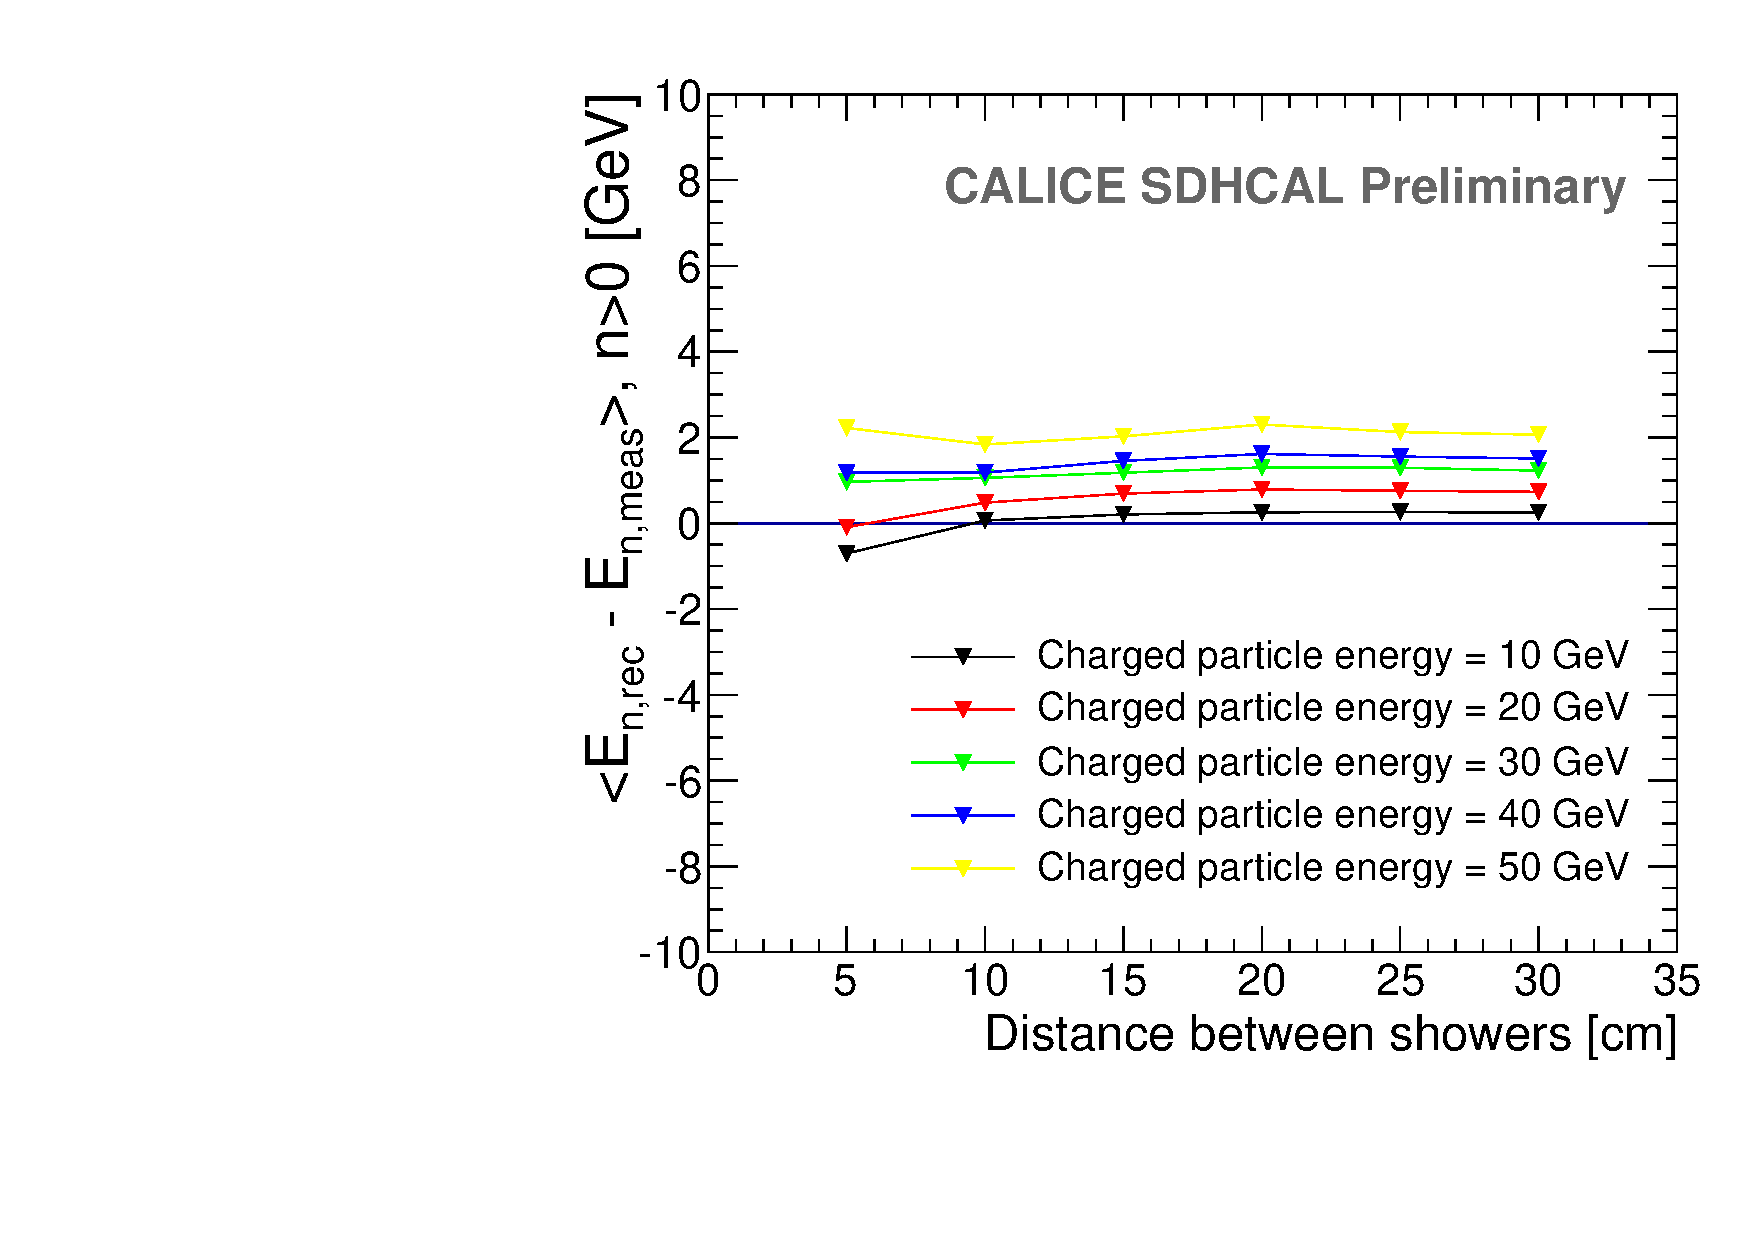
\includegraphics[width=0.48\linewidth]{OverlayEvent_NeutralEnergyDifferenceMeanNeutralEfficient.pdf}
    \end{center}
  \end{frame}
  
      
  \section{Conclusion and roadmap}
  
  %% Conclusion
  \begin{frame}
  \frametitle{Conclusion and roadmap}
    \begin{block}{Conclusion}
      \begin{itemize}
        \item Particle flow algorithm development based hadronic shower tree topology for the SDHCAL prototype
        \item Performance extraction for single particle - OK
        \item Performance extraction for two overlaid particles - OK till 5 cm
      \end{itemize}
      CALICE Analysis Note submitted : \textbf{CAN-054}
    \end{block}
    \begin{block}{Roadmap}
      \begin{itemize}
        \item Correction of some algorithms $\rightarrow$ re-extract performances (to do)
        \item Implementation for ILD-like detectors :
        \begin{itemize}
          \item Angular correction for connections (advanced)
          \item Implémentation for ECal (started)
          \item Muon reconstruction (to do)
          \item Photon reconstruction $\rightarrow$ GARLIC
          \item Energy calibration (ECal + HCal) (to do)
        \end{itemize}
        \item Physics performances :
        \begin{itemize}
          \item Jet energy resolution and scale (to do)
          \item W - Z separation
          \item Physics channel e+e- $\rightarrow$ HZ
        \end{itemize}
      \end{itemize}
    \end{block}
  \end{frame}


  \begin{frame}
  ~ \\
  ~ \\
  ~ \\
  ~ \\
  ~ \\
  ~ \\
    \centering \large Thanks for your attention !
  ~ \\
  ~ \\
  ~ \\    
  \end{frame}


  

  \section*{Backup}

  \begin{frame}
  \frametitle{\secname}
  \framesubtitle{Particle reconstruction and event selection}
    \begin{minipage}{0.4\linewidth}
      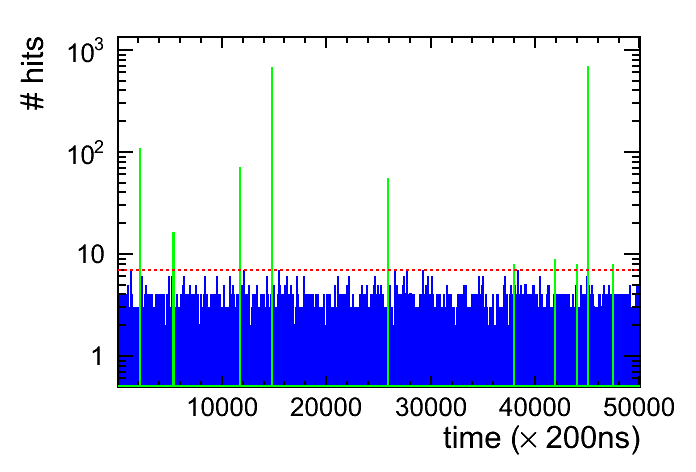
\includegraphics[width=\linewidth]{sdhcal_time_spectrum.png}
    \end{minipage} \hfill
    \begin{minipage}{0.58\linewidth}
      \begin{block}{Reconstruction : \textit{clustering} en temps}
        \begin{itemize}
          \item Minimum NHit : 7
          \item Time window : $\pm$ 2
        \end{itemize}
      \end{block}
    \end{minipage}
    \pause
    \begin{minipage}{0.6\linewidth}
      \begin{block}{Hadronic event selection}
        No cherenköv detector $\rightarrow$ topological selection
        \begin{itemize}
          \item Muon : NHit/N$_{layer}$ > 2.2
          \item Neutral particles : NHit $\in$ 5 first layers $\geq$ 4
          \item Radiative muons : $\frac{N_{touched~layers}/RMS>5cm}{N_{touched~layers}}$ < 20 \%
          \item Electrons : Z$_{begin}$ $\geq$ 5 and N$_{touched~layers}$ $\geq$ 30
        \end{itemize}
      \end{block}
    \end{minipage} \hfill
    \begin{minipage}{0.38\linewidth}
      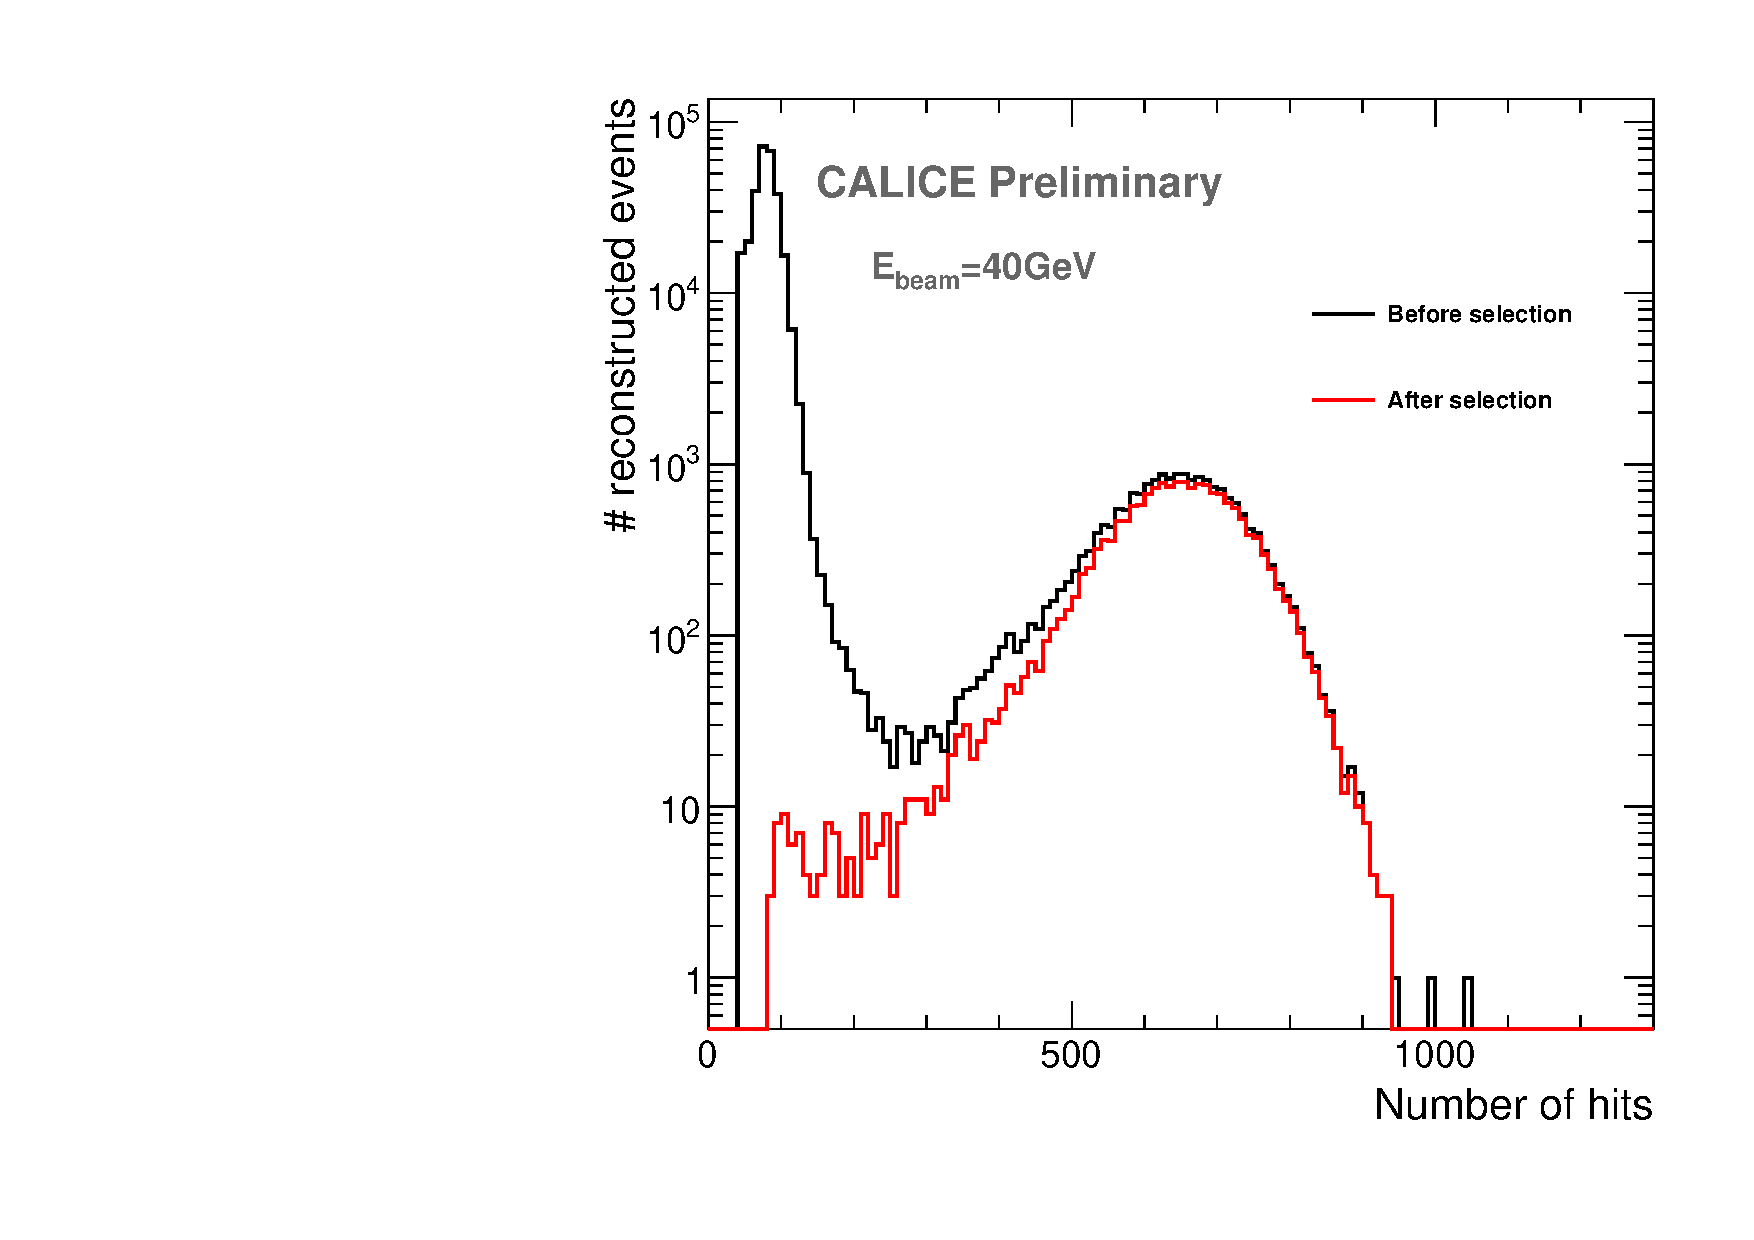
\includegraphics[width=\linewidth]{sdhcal_hadron_selection_40GeV.pdf}
    \end{minipage}
  \end{frame}
  

  \begin{frame}
  \frametitle{\secname}
  \framesubtitle{ArborPFA - Second connector iteration}
    \begin{minipage}{0.55\linewidth}
      \onslide<1->{
      \begin{block}{\textcircled{{\small 6}} et \textcircled{{\small 7}} Connector alignment}
        $\blacksquare$ From the previous tree structure, more connectors are created. 
      \end{block}
      }
      \onslide<2->{
      \begin{block}{\textcircled{{\small 7}} Connector cleaning 2}
        $\blacksquare$ Similar second connector cleaning. \\ ~ \\
        One difference : cleaning performed layer per layer  starting from the last one, with $\delta$ = 2 \\ ~ \\
        $\rightarrow$ Connector aligned with forward connections. \\
        \begin{center}
          \textbf{+}
        \end{center}
        $\rightarrow$ Tree structure !
      \end{block}
      }
    \end{minipage} \hfill
    \begin{minipage}{0.44\linewidth}
      \begin{center}
        \onslide<1->{
        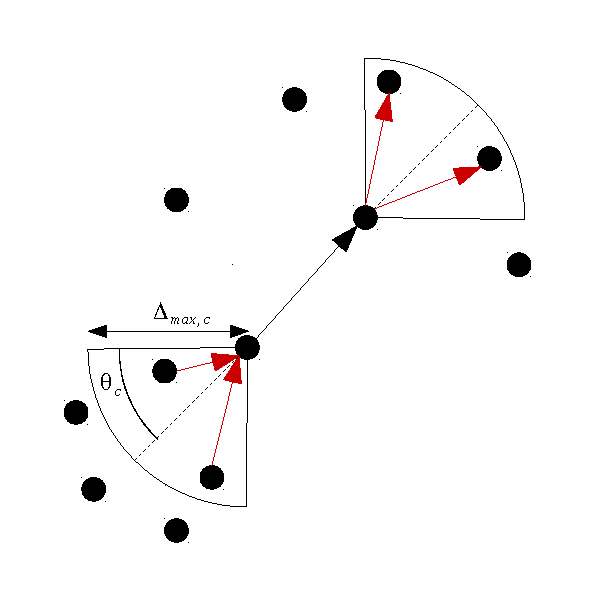
\includegraphics[width=0.7\linewidth]{ConnectorAlignment.pdf} \\ ~ \\
        }
        \onslide<2->{
        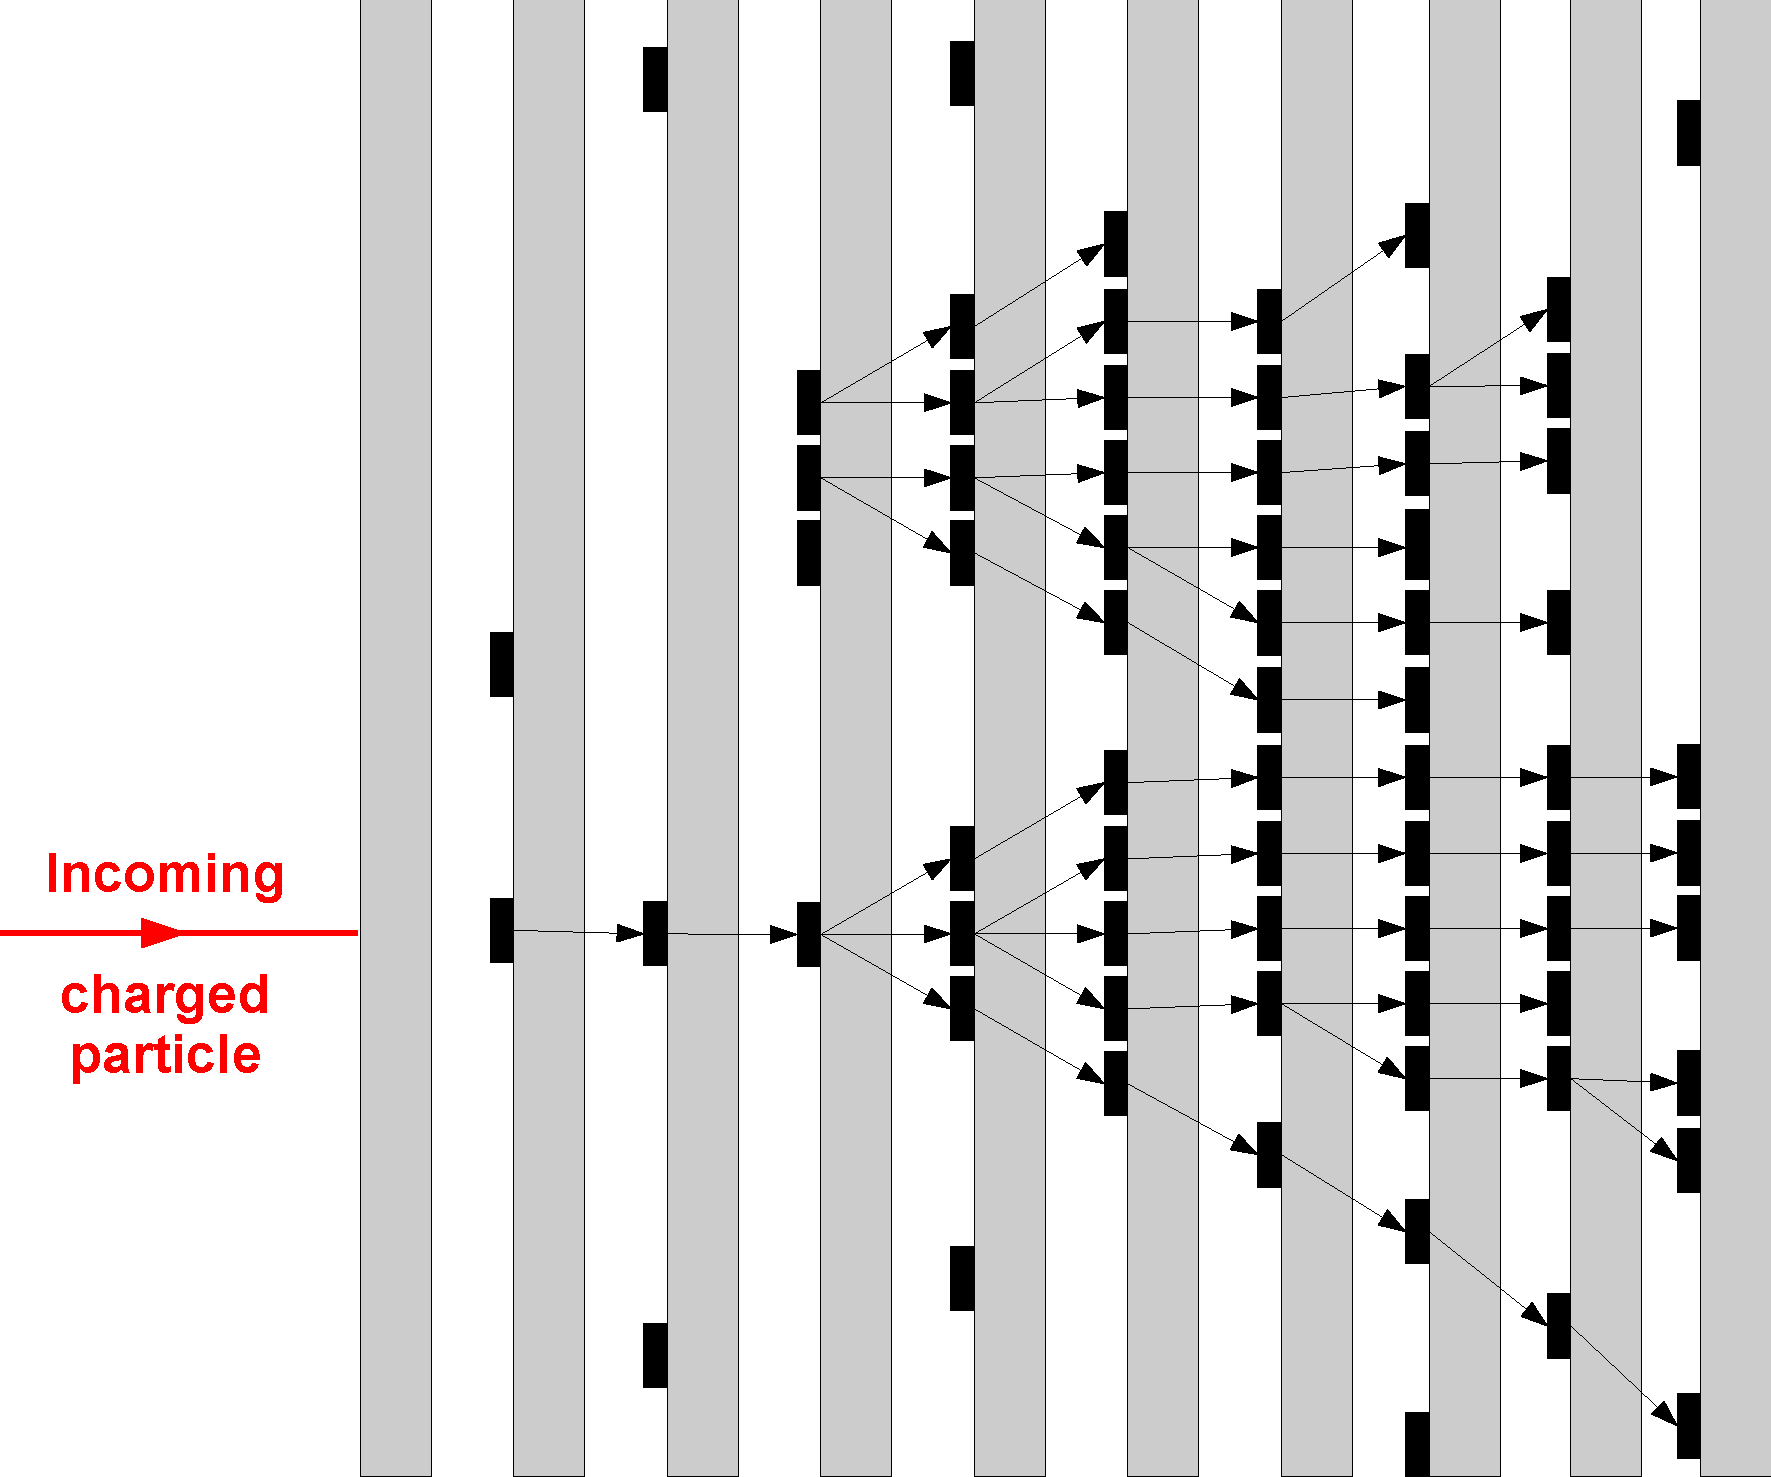
\includegraphics[width=0.9\linewidth]{ConnectorCleaning2.pdf}
        }
      \end{center}
    \end{minipage}
  \end{frame}
  
  
  \begin{frame}
  \frametitle{\secname}
  \framesubtitle{Overlaid hits approximation}
    \begin{center}
      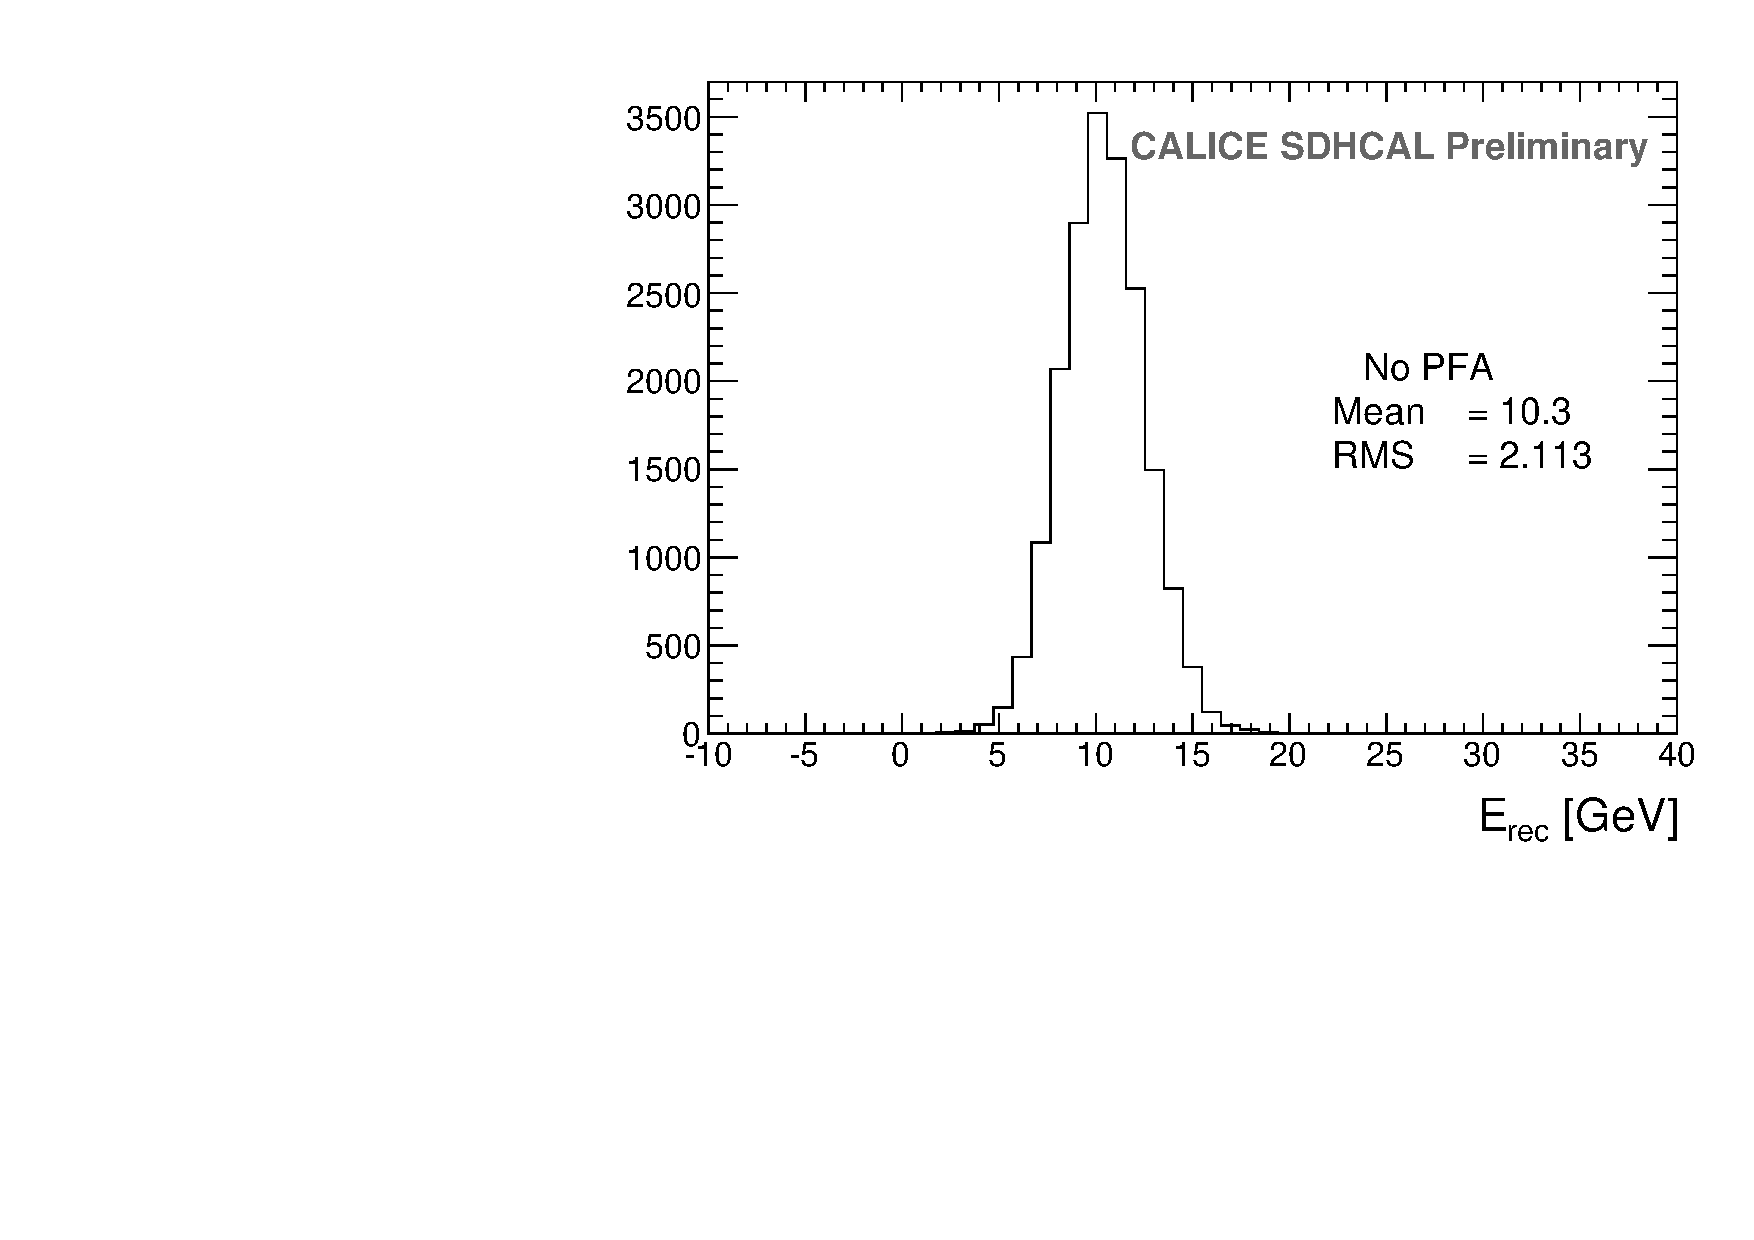
\includegraphics[width=0.52\linewidth]{SingleParticle_10GeV.pdf}
      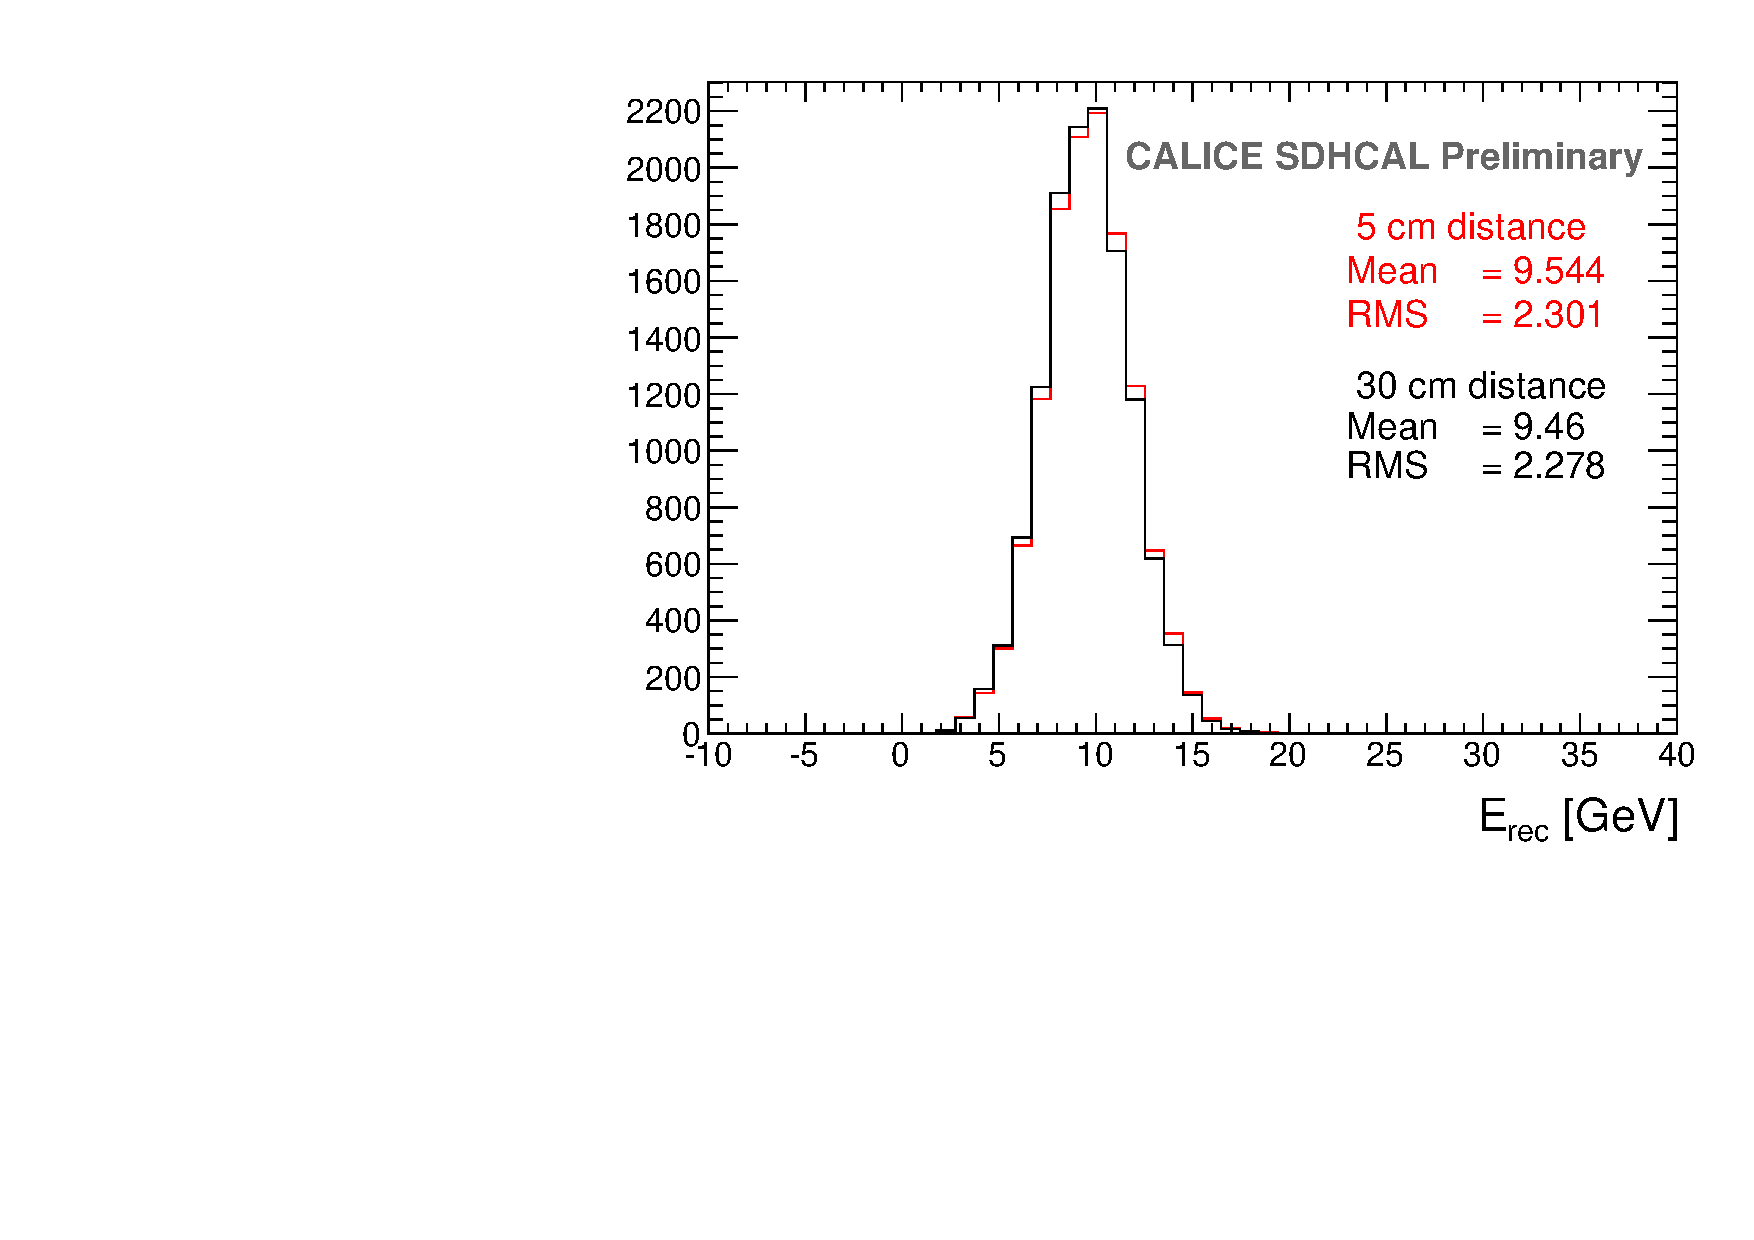
\includegraphics[width=0.52\linewidth]{OverlayEvent_OverlayCompare.pdf}
    \end{center}    
  \end{frame}
  

  \begin{frame}
  \frametitle{\secname}
  \framesubtitle{100 GeV jets statistics}
    \begin{center}
      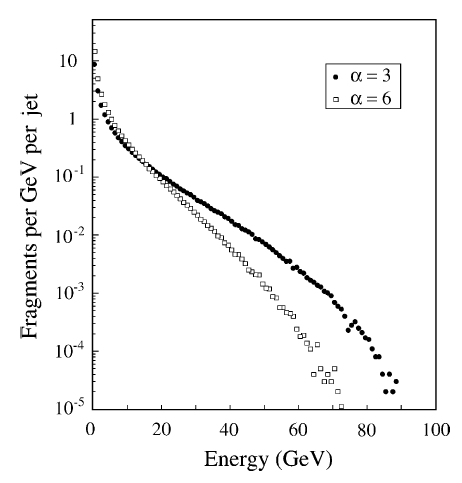
\includegraphics[width=0.34\linewidth]{jet_fragment_energy.png}
      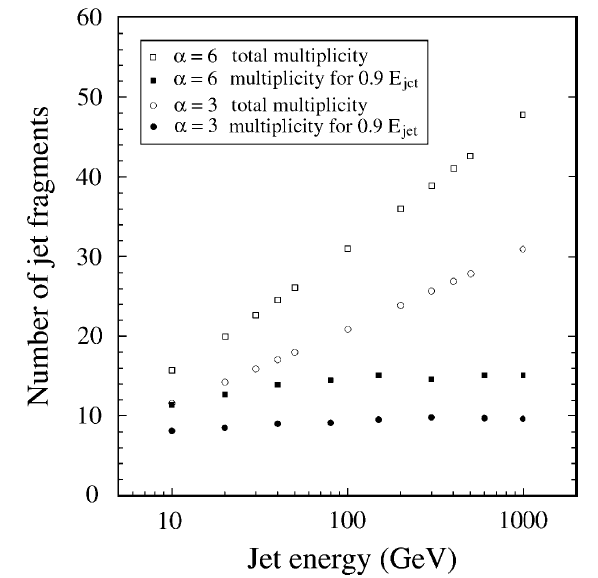
\includegraphics[width=0.34\linewidth]{jet_fragments.png}
      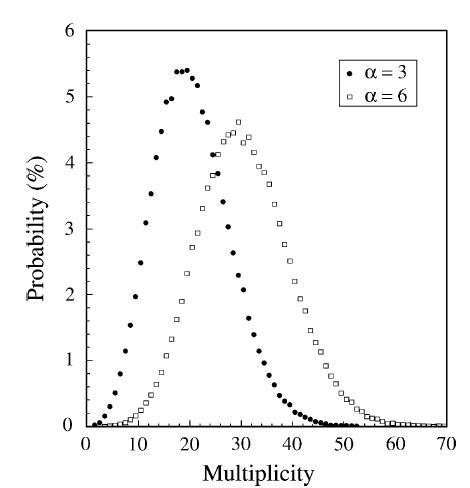
\includegraphics[width=0.34\linewidth]{jet_multiplicity.png}
    \end{center}    
  \end{frame}



\end{document}
